\documentclass[10pt,a4paper]{report}
\usepackage[latin1]{inputenc}
\usepackage{amsmath}
\usepackage{amsfonts}
\usepackage{amssymb}
\usepackage{hyperref} %pr inserer des liens internet

\usepackage{verbatim}%pour linsertion brute de commande LaTeX dans le texte
\usepackage{moreverb}

\usepackage{graphicx} %pour linsertion dimages

%Lignes ajout\'ees pour les documents en fran\c{c}ais, pour que soit prises en compte les particularit\'es de la typographie fran\c{c}aise; c'est aussi grâce \`{a} ce package que la date est affich\'ee automatiquement en fran\c{c}ais, que le titre de la table des mati\`eres est « Table des mati\`eres » et non « Contents », etc. Les deux lignes suivantes permettent d'avoir des caract\`eres correctement accentu\'es en toutes circonstances.
\usepackage[french]{babel}
\usepackage[latin1]{inputenc}


\usepackage{listings} %pr inserer du code
\usepackage{xcolor}
% pour une jolie insertion de code (https://www.sharelatex.com/project/51b8f1c34c2bd70430a90c23)
\lstset{
    backgroundcolor=\color{black!5}, % set backgroundcolor
    basicstyle=\footnotesize,% basic font setting
    language=C++,
    %basicstyle=\ttfamily\small,
    breaklines=true,
    prebreak=\raisebox{0ex}[0ex][0ex]{\ensuremath{\hookleftarrow}},
    frame=lines,
    showtabs=false,
    showspaces=false,
    showstringspaces=false,
    keywordstyle=\color{red}\bfseries,
    stringstyle=\color{green!50!black},
    commentstyle=\color{gray}\itshape,
    numbers=left,
    captionpos=t,
    escapeinside={\%*}{*)}
}



%Pour faire un index
\usepackage{makeidx}
%Pour faire un index 
\makeindex

\title{OGRE}
\author{O}


\begin{document}



\part*{Avant-Propos}
\section*{Pr\'esentation du document}
This document is a re-lecture of the tutorial \href{http://fr.openclassrooms.com/informatique/cours/decouvrez-ogre-3d}{''D\'ecouvrez Ogre 3D''}. The original tutorial was written by Julien Chichignoud on \href{fr.openclassrooms.com}{Openclassroom} (aka ''Le site des z\'eros'').\newline

Writing this document is an attempt to make something like an active reading, and thus have a more attentive lecture and deepest understanding of Ogre's concepts. We modified a lot (sentences, structure, ...) but the essence is the same as the original tutorial.\newline

We wish to highligh the fact that this document is a personal interpretation, and a in progress work.\newline

The original tutorial is in French and as we are spending most of our strength in the comprehension of Ogre we did not take time to translate the original tutorial in French.\newline


\section*{Licence}
The original tutorial is released under the 
\href{http://creativecommons.org/licenses/by-nc-sa/2.0/}{Creative Common licence} and so is also released this document.\newline

The rest of the document will be now in French, sorry for those who cannot take advantage of the document.


\part{Bases de Ogre}

%---------------------------------------------------------------------------------------------------------------

%!!! 3OGRE3 n est pas centre dans le titre qui suit
\chapter{Installation, Premier programme}

\section{Premier pas}
\subsection{Sources}
J'ai d'abord voulu suivre le tutoriel du site du z\'ero
\url{http://fr.openclassrooms.com/informatique/cours/decouvrez-ogre-3d/}\newline

Mais ce tutoriel du site des z\'eros semble plus ax\'e visual studio, par contre un lien est donn\'e pour la compilation de projets sous Ubuntu \url{http://geenux.wordpress.com/2010/03/18/installation-de-ogre-1-7-et-compilation-avec-cmake-sous-ubuntu/}


\subsection{Installation}
Installation avec synaptic des packages suivants:
\begin{enumerate}
\item libogre-dev
\item ogre-samples
\item ogre-samples-data
\item libogre-1.7.4
\item libois-1.3.0
\item libois-dev 
\end{enumerate}






\section{Premiere compilation}

\subsection{Premier programme}

\begin{itemize}
\item Cr\'eation d'un r\'epertoire contenant les fichiers suivants:
\end{itemize}

\begin{lstlisting}
Hraesvelg:~/Documents/workspace/3D/OGRE/ExampleApplication$ ls -l
total 24
-rw-rw-r-- 1 olivier olivier 1109 fvr. 23 12:16 CMakeLists.txt
-rw-rw-r-- 1 olivier olivier  844 fvr. 23 12:02 helloworld.cpp
-rw-rw-r-- 1 olivier olivier 4894 fvr. 23 12:18 Makefile
-rw-r--r-- 1 olivier olivier  446 fvr. 23 12:20 plugins.cfg
-rw-r--r-- 1 olivier olivier 1391 fvr. 23 12:20 resources.cfg
\end{lstlisting}


\begin{itemize}
\item helloworld.cpp:
\end{itemize}

\begin{lstlisting}
#include ''ExampleApplication.h''
 
class TutorialApplication: public ExampleApplication
{
protected:
public:
    TutorialApplication()
    {
    }
 
    ~TutorialApplication()
    {
    }
protected:
    void createsc\`ene(void)
    {
    }
};
 
#if OGRE_PLATFORM == OGRE_PLATFORM_WIN32
#define WIN32_LEAN_AND_MEAN
#include ''windows.h''
 
INT WINAPI WinMain( HINSTANCE hInst, HINSTANCE, LPSTR strCmdLine, INT )
#else
int main(int argc, char **argv)
#endif
{
    // Create application object
    TutorialApplication app;
 
    try {
        app.go();
    } catch( Exception& e ) {
#if OGRE_PLATFORM == OGRE_PLATFORM_WIN32
        MessageBox( NULL, e.what(), ''An exception has occurred!'', MB_OK | MB_ICONERROR | MB_TASKMODAL);
#else
        fprintf(stderr, ''An exception has occurred: %s\n'',
                e.what());
#endif
    }
 
    return 0;
}
\end{lstlisting}



\begin{itemize}
\item CMakeLists.txt est une copie modifi\'ee du CMakeLists.txt donn\'ee dans le tutoriel de compilation sous Ubuntu. Les lignes commencant par \# \~ sont les lignes originales que j'ai du modifier.
\end{itemize}





%!!! CE QUI SUIT EST EN COM PARCE QUE LA COMPIL BUGGE DESSUS
\begin{lstlisting}
project(helloworld)
cmake_minimum_required(VERSION 2.6)

\# \~ set(CMAKE_MODULE_PATH ''/usr/lib/OGRE/cmake/'')
set(CMAKE_MODULE_PATH ''/usr/share/OGRE/cmake/modules'')

#set(CMAKE_CXX_FLAGS ''-Wall -W -Werror -ansi -pedantic -g'')

# Il s sagit du tutoriel d exemple, qui utilise quelques fichiers predefini de Ogre. Il faut indiquer a cmake o\'{u} se trouvent les includes en question
# \~ include_directories (''/usr/share/OGRE/Samples/Common/include/'')
include_directories (''/usr/share/OGRE-1.7.4/Samples/Common/include/'')

# Bien sur, pour compiler Ogre, il faut le chercher, et definir le repertoire contenant les includes.
find_package(OGRE REQUIRED)
include_directories (${OGRE_INCLUDE_DIRS})

# L'exemple depend aussi de OIS, une lib pour gerer la souris, clavier, joystick...
find_package(OIS REQUIRED)

# On definit les sources qu'on veut compiler
SET(SOURCES
helloworld.cpp)

# On les compile
add_executable (
helloworld ${SOURCES}
)

# Et pour finir, on lie l'executable avec les librairies que find_package nous a gentillement trouve.
target_link_libraries(helloworld ${OGRE_LIBRARY} ${OIS_LIBRARY})
%\end{lstlisting}


plugins.cfg et resources.cfg sont copi\'es de /usr/share/OGRE-1.7.4

\subsection{Compilation}
les commandes \`{a} faire sont:
\begin{itemize}
\item cmake.
\item make
\item./helloworld
\end{itemize}

\section{Premiere compilation sous CodeBlocks}
A tenter!!!!\newline
\url{http://fr.openclassrooms.com/informatique/cours/decouvrez-ogre-3d/configuration-d-un-projet-3}

\section{Premiere compilation sous kDevelop}
J'ai suivi\newline
\url{http://www.ogre3d.org/tikiwiki/tiki-index.php?page=Setting+Up+An+Application+-+KDevelop+-+Linux}.\newline
Je copie dans le r\'epertoire ogretest le r\'epertoire d'exemple Sample\_Water. Le processus foire.




\section{Code de base}
\subsection{Source}
\url{http://fr.openclassrooms.com/informatique/cours/decouvrez-ogre-3d/le-code-de-base-1}

Ce code de base est en fait le m\^eme que celui fait dans le chapitre Premiere Compilation, sauf qu'alors on avait que un seul fichier cpp, on rajoute i\c{c}i un fichier.h qui est inclus dans le fichier main.cpp.




%---------------------------------------------------------------------------------------------------------------
\chapter{Ins\'erer des objets dans la sc\`ene }

\section{les entit\'es}

\subsection{Une entit\'e c'est quoi}
Une entit\'e est l'ensemble des informations attach\'ees aux polygones constituant un objet 3D.\newline
Un Mesh \'etant l'ensemble des polygones constituant un objet 3D, une entit\'e est l'ensemble des informations attach\'ees \`{a} un Mesh:

\begin{itemize}
\item les vertices (sommets des polygones),
\item les textures,
\item un squelette si le modele est sujet \`{a} des animations
\item...\newline
\end{itemize}


Tous les objets solides qui apparaissent \`{a} l'\'ecran sont donc des entit\'es et sont repr\'esent\'es par une seule et m\^eme classe dans Ogre: la classe Entity.

\subsection{Le sceneManager}
C est au sceneManager que revient la t\^{a}che de cr\'eer tous les objets que peut contenir la sc\`ene (tous les mod\`eles, lumi\`eres, cam\'era et autres objets) et de nous permettre ensuite d'y acc\'eder.\newline
Par cons\'equent, l'insertion d'objets dans la sc\`ene passe toujours par lui (ou par l'un des \'el\'ements d\'ej\`{a} ins\'er\'es) et par les m\'ethodes qu'il propose pour cela.
Il en existe diverses variantes en fonction de la sc\`ene que l'on veut r\'ealiser; selon que celle-ci sera par exemple en int\'erieur ou en ext\'erieur, par exemple.

Toutes les applications Ogre doivent donc avoir un sceneManager pour pouvoir fonctionner, puisque c'est lui qui s'occupe de tout ! La classe ExampleApplication ne fait pas exception et poss\`ede donc un attribut msceneMgr, qui est un pointeur sur le sceneManager de l'application et qui nous permettra dans les parties suivantes d'agr\'ementer notre sc\`ene avec des objets.


\subsection{Cr\'eer une entit\'e}

L'entit\'e doit \^etre cr\'e\'ee par le sceneManager pour pouvoir \^etre ajout\'ee \`{a} la sc\`ene. La m\'ethode createEntity() permet de faire cela.
\begin{lstlisting}
Entity *head= msceneMgr->createEntity(''Tete'',''ogrehead.mesh'');
\end{lstlisting}\footnote{Pourquoi utilise t on -> pour appeler une m\'ethode d'une classe?}

\begin{itemize}
\item Le premier param\`etre est le nom que vous souhaitez donner au mesh. Ce nom doit \^etre unique!
\item Le second param\`etre est le nom du fichier que vous voulez charger. Notez l'extension.mesh, qui est le format de fichiers pour les mod\`eles reconnu par Ogre.
\end{itemize}




Le fichier sp\'ecifi\'e (avec le deuxi\`eme param\`etre) se trouve, accompagn\'e d'autres mod\`eles d'exemples, dans le dossier OgreSDK/media/models, qui doit \^etre correctement renseign\'e dans le fichier resources.cfg pour qu'Ogre puisse le trouver lors de l'ex\'ecution.\footnote{Mais \`a quoi sert ce fichier .mesh?}

Le mesh a \'et\'e ajout\'e \`{a} la sc\`ene mais il nous manque encore une chose avant de pouvoir l'afficher \`{a} l'\'ecran...













\section{Les Noeuds de la sc\`ene}



\subsection{L'utilit\'e des Noeuds}

Dans Ogre, lorsque l'on souhaite manipuler une entit\'e (un personnage, une lumi\`ere, une cam\'era...), les d\'eplacements que l'on veut effectuer se font par l'interm\'ediaire d'un noeud de sc\`ene, ou sceneNode.

Un sceneNode est un objet invisible auquel on va pouvoir attacher un nombre ind\'efini d'entit\'es, lesquelles deviennent solidaires de ce noeud et subissent donc les m\^eme transformations que lui. C'est donc une sorte de conteneur qui contient les informations de positionnement de chacune des entit\'es de la sc\`ene qui lui sont rattach\'ees.

Bien s\^ur on pourrait d\'eplacer nos entit\'es directement mais avec un noeud on pourra d\'eplacer en une fois toutes les entit\'es attach\'ees au noeud.

Quoi qu'il en soit, attacher chaque entit\'e \`{a} un noeud est primordial, sans quoi elle ne s'affichera pas dans votre sc\`ene!



\subsection{Cr\'eer un noeud}

Pour cr\'eer un noeud de sc\`ene on devra passer par un noeud d\'ej\`{a} existant, ce qui va nous permettre d'avoir des relations d'h\'eritage entre nos noeuds.\newline

On utilisera une m\'ethode d\'edi\'ee:

\begin{lstlisting}
sceneNode *noeudEnfant = noeudParent->createChildsceneNode(''enfant'', Vector3::ZERO, Quaternion::IDENTITY);
\end{lstlisting}


Mais comment fait-on pour le premier noeud\index{noeud} qu'on va cr\'eer ? Le noeud ''racine'' existe d\`es que le sceneManager est cr\'e\'e, c'est un noeud comme un autre avec les m\^eme \footnote{''les m\^eme'' faut il un ''s'' \`{a} ''m\^eme'' ?} m\'ethodes mais ce noeud est unique.\newline

Nous r\'ecup\'erons ce noeud racine de la sc\`ene  \`{a} l'aide de l'instance du sceneManager:
\begin{lstlisting}
sceneNode *node= msceneMgr->getRootsceneNode()->createChildsceneNode(''nodeTete'', Vector3::ZERO, Quaternion::IDENTITY);
\end{lstlisting}

La m\'ethode getRootsceneNode() nous permet de r\'ecup\'erer un pointeur sur le noeud racine unique de la sc\`ene. On appelle ensuite sa m\'ethode createChildsceneNode pour lui ajouter un nouveau noeud fils.

Notez qu'aucun des param\`etres de la m\'ethode n'est obligatoire, pour information:
\begin{itemize}
\item Le premier argument est le nom que vous voulez donner \`{a} votre noeud. Sur le m\^eme principe que les entit\'es ce nom pourra \^etre utilis\'e pour r\'ecup\'erer un pointeur vers le noeud en question. 
\item Le deuxi\`eme argument est la position initiale du noeud.
\item Le troisi\`eme argument est le quaternion avec lequel vous voulez initialiser votre noeud.
\end{itemize}
	

Sachez pour le moment qu'un quaternion est un objet math\'ematique qui permet de faire faire aux objets des rotations dans l'espace\footnote{Que des rotations?}. Quaternion::IDENTITY \footnote{comment \'ecrire Quaternion::IDENTITY de manière \'el\'egante?}lui dit de ne pas faire de rotation.\newline

Avec ce code en main, vous pouvez simplement attacher l'entit\'e pr\'ec\'edemment cr\'e\'ee au noeud avec la ligne suivante:

\begin{lstlisting}
node->attachObject(head);
\end{lstlisting}

En compilant, vous devriez voir la t\^ete d'un ogre au milieu de l'\'ecran. Vous pouvez d\'eplacer la cam\'era avec Z, S, Q, D et la souris pour voir ce que \c{c}a donne de plus pr\`es.



\subsection{Code}

\subsubsection{PremiereApplication.cpp}
\begin{lstlisting}[caption={PremiereApplication.cpp: Instanciation d'entit\'e}]
#include "PremiereApplication.h"

void PremiereApplication::createScene()
{
    //creation d une entite
    Entity *head= mSceneMgr->createEntity("Tete", "ogrehead.mesh" );
    
    //creation d un noeud
    SceneNode *node= mSceneMgr->getRootSceneNode( )->createChildSceneNode( "nodeTete " , Vector3::ZERO, Quaternion::IDENTITY);
    
    node->yaw(Radian(Math::PI));
    node->yaw(Radian(Math::PI));

    Vector3 position = Vector3(30.0, 50.0, 0.0);
    node->setPosition(position);

    node->setPosition(30.0, 50.0, 0.0); 
    node->translate(-30.0, 50.0, 0.0); 
    
    
    //attachement de l entite au noeud
    node->attachObject ( head );
}
\end{lstlisting}








\section{Cr\'eer un mesh}

Nous pouvons rajouter un sol \`{a} notre sc\`ene, pour cela nous allons cr\'eer nous-m\^emes\footnote{il faut un ''s'' \`a  nous-m\^emes?} un nouveau mesh. \'Etant donn\'e que nous n'avons besoin que d'un plan pour le sol, le mesh peut tr\`es simplement \^etre cr\'eer dans le code de notre application.



\subsection{Le mesh}

Il existe une classe Plane\footnote{de m\^eme que pour quaternion.entity marquer les noms de classe de manière \'el\'egante pour les discerner du texte serait bien} qui va nous permettre de g\'en\'erer... un plan qui repr\'esentera le sol.\footnote{En plus de la classe Plane, vous trouverez aussi des classes Box (pour les cubes) et Sphere qui fonctionnent sur le m\^eme principe.}\newline

Pour cr\'eer un plan nous appelons Plane avec les param\`etres suivants:
\begin{itemize}
\item le premier param\`etre permet de d\'efinir le vecteur normal au plan \`{a} cr\'eer (ici l'axe Y pour que notre plan soit horizontal).
\item le second param\`etre est la distance \`{a} l'origine de la sc\`ene dans le sens du vecteur normal  (ici, je mets 0 pour que mon mesh plan soit centr\'e). 
\end{itemize}

\begin{lstlisting}
	Plane plan(Vector3::UNIT_Y, 0);
\end{lstlisting}

Une fois le plan cr\'e\'e, il faut que l'on cr\'ee un mesh, c'est-\`{a}-dire l'objet 3D en lui-m\^eme (la repr\'esentation du plan) qui sera visible dans la sc\`ene.
Pour cela, on utilise le Mesh Manager, qui va s'occuper de cr\'eer les faces de notre mesh.

\begin{lstlisting}
MeshManager::getSingleton().createPlane(''sol'', ResourceGroupManager::DEFAULT_RESOURCE_GROUP_NAME, plan, 500, 500, 1, 1, true, 1, 1, 1, Vector3::UNIT_Z);
\end{lstlisting}

Quelques explications sur cette ligne s'imposent. 
\begin{itemize}
\item Tout d'abord, la m\'ethode statique getSingleton() permet de r\'ecup\'erer un objet instanci\'e de fa\c{c}on unique, donc ici notre MeshManager.
\item Les deux premiers param\`etres correspondent respectivement au nom que l'on veut donner \`{a} notre mesh et au nom du groupe auquel on veut qu'il appartienne. 
\item Suivent ensuite le nom du plan \`{a} mod\'eliser, puis la largeur et la hauteur qu'il doit avoir, puis le nombre de subdivisions du plan dans ces deux sens. Plus il y a de subdivisions, plus il y a de polygones dans notre mesh. 
\item Le bool\'een suivant indique que les normales sont perpendiculaires au plan.
\item Les trois param\`etres suivants sont le nombre de textures que l'on va pouvoir assigner au plan, puis le nombre de fois que la texture sera r\'ep\'et\'ee dans les deux directions. 
\item le dernier param\`etre est le vecteur indiquant la direction du haut du mesh. Attention: il ne faut pas le confondre avec la normale du plan, qui est diff\'erente.
\end{itemize}

Il reste encore des param\`etres par d\'efaut que l'on verra plus tard.

Enfin, nous allons revenir vers un code connu: nous allons cr\'eer l'entit\'e qui repr\'esentera le plan. C'est le m\^eme principe que tout \`{a} l'heure:
\begin{itemize} 
\item tout d'abord, on cr\'ee une entit\'e \`{a} partir du sc\`ene Manager en la nommant et en lui indiquant le mesh \`{a} utiliser. 
\item On cr\'ee ensuite un nouveau noeud \`{a} partir du noeud racine et on l'attache \`{a} notre entit\'e.
\end{itemize}

\begin{lstlisting}
//creation d'une entite
Entity *ent= msceneMgr->createEntity(''EntiteSol'', ''sol'');

//creation d'un nouveau noeud
node = msceneMgr->getRootsceneNode()->createChildsceneNode();

//on attache le noeud a notre entite
node->attachObject(ent);
\end{lstlisting}




\subsection{Le mat\'eriau}

Nous allons finir en ajoutant une texture au sol: de l'herbe. Pour cela, il suffit de rajouter la ligne suivante apr\`es la cr\'eation de l'entit\'e:
\begin{lstlisting}
ent->setMaterialName(''Examples/GrassFloor'');
\end{lstlisting}

Si vous voulez conna\^itre les mat\'eriaux fournis avec Ogre, il vous suffit d'aller dans le dossier media/materials/scripts. Ici, on prend le mat\'eriau GrassFloor enregistr\'e dans le fichier Examples.material. 

Les textures correspondantes se trouvent dans le dossier media/materials/textures, si vous voulez faire des essais.


Vous pouvez maintenant ex\'ecuter votre programme.

Lancez l'application et remontez la cam\'era avec la souris et les touches de d\'eplacement, vous devriez voir quelque chose ressemblant \`{a} la capture suivante.

Image utilisateur

Euh... La t\^ete d'Ogre est coup\'ee par le sol en herbe...

En effet, notre plan est centr\'e sur l'origine de la sc\`ene, et l'on a aussi plac\'e notre t\^ete \`{a} l'origine. Mais quelle partie de la t\^ete est \`{a} l'altitude 0 ?

Ici, c'est donc un point au milieu de la t\^ete, puisque le plan d'herbe passe par l\`{a}.
Cependant, ce point n'est pas n\'ecessairement au milieu de l'objet que vous int\'egrez. Cela d\'epend de la personne qui a mod\'elis\'e l'objet et qui a donc d\'ecid\'e par rapport \`{a} quel point on allait d\'efinir la position du mesh. Pour un personnage, on pourrait mettre ce point \`{a} ses pieds, pour que l'altitude 0 corresponde effectivement au moment o\`{u} le personnage touche le sol avec ses pieds.

Pour corriger cela, il va falloir remonter notre noeud li\'e \`{a} notre entit\'e. C'est l'objet du prochain chapitre.

































\subsection{Code}

\subsubsection{PremiereApplication.cpp}
\begin{lstlisting}[caption={PremiereApplication.cpp: Cr\'eation d'un sol}]
#include "PremiereApplication.h"

void PremiereApplication::createScene()
{
    //creation d une entite
    Entity *head= mSceneMgr->createEntity("Tete", "ogrehead.mesh" );
    
    //creation d un noeud
    SceneNode *node= mSceneMgr->getRootSceneNode( )->createChildSceneNode( "nodeTete " , Vector3::ZERO, Quaternion::IDENTITY);
    
    node->yaw(Radian(Math::PI));
    node->yaw(Radian(Math::PI));

    //setPosition place le noeud aux coord passees en parametres
    Vector3 position = Vector3(30.0, 50.0, 0.0);
    node->setPosition(position);

    node->setPosition(30.0, 50.0, 0.0); 
    /*equivalent a
    Vector3 position = Vector3(30.0, 50.0, 0.0);
    node->setPosition(position);
    */

    //deplace le noeud par rapport a sa position actuelle
    node->translate(-30.0, 50.0, 0.0); //par defaut la trnslt se fait par rap a TS_WORLD
   
    //attachement de l entite au noeud
    node->attachObject ( head );

    //creation d un plan
    Plane plan(Vector3::UNIT_Y, 0);

    //creation d un mesh cad l objet 3d visible ds la scene
    MeshManager::getSingleton().createPlane("sol",
                ResourceGroupManager::DEFAULT_RESOURCE_GROUP_NAME,
                plan, 500, 500, 1, 1, true, 1, 1, 1, Vector3::UNIT_Z); 

    //entite qui representera le plan
    Entity *ent= mSceneMgr->createEntity("EntiteSol", "sol");

    //ajout du materiau a l entite
    ent->setMaterialName("Examples/GrassFloor");//texture de pelouse
    /*les differents materiaux sont sous /media/materials/scritps, par ex:
    ent->setMaterialName("Examples/WaterStream");//texture d eau animee*/

    //creation d un noeud
    node = mSceneMgr->getRootSceneNode()->createChildSceneNode();
    node->attachObject(ent);
}


\end{lstlisting}

A cause de la position de la cam\'era, il se peut alors que le sol ne soit pas visible.



%---------------------------------------------------------------------------------------------------------------
\chapter{Se rep\'erer dans l'espace}


\section{Le syst\`eme de coordonn\'ees}


\subsection{Le rep\`ere ''main droite''}

Le rep\`ere est orthogonal et orthonorm\'e (les axes/les vecteurs directeurs de ces axes sont perpendiculaires les uns aux autres et de longueur 1)



\subsection{Pourquoi main droite ?}

Regardez votre main droite.
\begin{itemize} 
\item Votre pouce repr\'esente l'axe X, 
\item votre index repr\'esente l'axe Y,
\item votre majeur repr\'esente l'axe Z. 
\end{itemize}

La direction dans laquelle pointe chacun de vos doigts d\'efinit le sens de chaque axe.

Image utilisateur cf(\url{fr.openclassrooms.com/informatique/cours/decouvrez-ogre-3d/le-systeme-de-coordonnees-1})





\subsection{Rep\`ere local, rep\`ere absolu}

Pour l'instant, nous n'avons toujours pas d\'efini comment le rep\`ere \'etait plac\'e dans la sc\`ene. C'est une question de convention adopt\'ee pour les applications 3D	pour le rep\`ere de la sc\`ene:
\begin{itemize}
\item l'axe Y dirig\'e vers le haut 
\item les axes X et Z dans un plan horizontal.
\end{itemize}

Seulement\footnote{comment faire pour sauter une ligne avant le ''Seulement''?}, la sc\`ene n'est pas la seule \`{a} avoir son rep\`ere. En effet, chaque objet poss\`ede son propre rep\`ere appel\'e rep\`ere local. Lorsque l'objet se d\'eplace ou tourne sur lui-m\^eme, le rep\`ere local fait de m\^eme. L'orientation du rep\`ere local est la suivante: 
\begin{itemize}
\item l'axe Y est dirig\'e vers le haut de l'objet, pour la sc\`ene, 
\item l'axe X est dirig\'e vers sa droite
\item l'axe Z vers l'arri\`ere de l'objet.
\end{itemize}
	


Ci-dessous\footnote{comment faire pour sauter une ligne avant le ''Ci-dessous''?}, j'ai repr\'esent\'e en noir le rep\`ere de la sc\`ene, et en bleu le rep\`ere local de la voiture, en respectant la convention que j'ai donn\'ee.
Image utilisateur cf(\url{fr.openclassrooms.com/informatique/cours/decouvrez-ogre-3d/le-systeme-de-coordonnees-1})

Nous verrons \`{a} quoi servent ces diff\'erents rep\`eres lorsque l'on commencera \`{a} d\'eplacer nos objets.








\subsection{Yaw, pitch, roll}

yaw pitch roll sont les d\'esignations anglaises pour les rotations autour des axes Y, X et Z respectivement. On peut traduire ces termes par lacet (yaw), tangage (pitch) et roulis (roll), qui sont utilis\'es par exemple en a\'eronautique ou en navigation.

Ces trois termes se retrouveront dans les noms qu'Ogre donne aux m\'ethodes permettant d'effectuer des rotations. 

Voici tout de suite un sch\'ema illustrant les rotations qui s'appliquent \`{a} chaque axe:

Image utilisateur cf(\url{fr.openclassrooms.com/informatique/cours/decouvrez-ogre-3d/le-systeme-de-coordonnees-1})


Tout comme l'orientation des axes de notre rep\`ere, il y a un sens direct et un sens indirect pour les rotations! Vous tournerez dans le sens direct lors  d'une rotation contraire\footnote{''rotation contraire'' <-> ''sens direct'', est ce correct?} au sens des aiguilles d'une montre.

Pour effectuer une rotation, on appelle la m\'ethode correspondante pour le noeud:
\begin{lstlisting}
	node->yaw(Radian(Math::PI));
\end{lstlisting}

Ceci fera faire un demi-tour au noeud par rapport \`{a} son axe vertical tandis que les m\'ethodes pitch() et roll() s'utilisent de fa\c{c}on analogue pour les autres axes.

La rotation se fait par d\'efaut par rapport au rep\`ere local. Il faut renseigner le second param\`etre si vous voulez qu'il en soit autrement (voir la section suivante).

Les angles doivent \^etre entr\'es en radians. Pour utiliser tout de m\^eme des degr\'es dans Ogre, vous devrez utiliser la classe Degree. La ligne de code pr\'ec\'edente est \'equivalente \`{a} ceci:
\begin{lstlisting}
	node->yaw(Degree(180));
\end{lstlisting}









\section{D\'eplacer des objets}




\subsection{Bouger un noeud de sc\`ene}

Nous allons maintenant d\'eplacer notre t\^ete d'ogre pour v\'erifier la th\'eorie et enfin sortir notre t\^ete de terre!

Pour cela, nous allons donc passer par le noeud auquel est rattach\'e notre mesh. Celui-ci poss\`ede deux m\'ethodes qui peuvent nous servir.




\subsection{setPosition()}

La m\'ethode setPosition() prend en param\`etres les trois coordonn\'ees X, Y et Z du point auquel on d\'esire placer le noeud. On peut aussi lui passer un Vector3, qui contiendra lui-m\^eme ces coordonn\'ees.

Les deux codes suivants sont donc \'equivalents.
\begin{lstlisting}
	Vector3 position = Vector3(30.0, 50.0, 0.0);
	node->setPosition(position);
\end{lstlisting}

ou
\begin{lstlisting}
	node->setPosition(30.0, 50.0, 0.0);
\end{lstlisting}

La t\^ete s'est maintenant d\'eplac\'ee vers la droite de 30 unit\'es et de 50 unit\'es vers le haut.




\subsection{translate()}

La m\'ethode translate() d\'eplace le noeud par rapport \`{a} sa position actuelle plut\^ot que par rapport \`{a} l'origine de la sc\`ene.

Elle prend les m\^emes param\`etres que la m\'ethode setPosition(), mais avec un param\`etre suppl\'ementaire, d\'efini par d\'efaut, indiquant le noeud par rapport auquel on va se d\'eplacer.
\begin{lstlisting}
	node->translate(-30.0, 50.0, 0.0);
\end{lstlisting}

En ajoutant cette ligne apr\`es la pr\'ec\'edente, notre objet se retrouve donc maintenant \`{a} la position (0, 100, 0) dans la sc\`ene, ce qui est suffisant pour qu'il surplombe son petit jardin.

Image utilisateur

Le param\`etre suppl\'ementaire (par rapport \`{a} setPosition) permet de d\'efinir par rapport \`{a} quel rep\`ere on va d\'eplacer le noeud.

Les trois valeurs possibles sont:
\begin{lstlisting}
    Node::TS_LOCAL //va deplacer le noeud par rapport au repere local
    Node::TS_PARENT //va deplacer le noeud au repere du noeud parent
    Node::TS_WORLD //va deplacer le noeud au repere de la scene, qui est le repere absolu.
\end{lstlisting}\footnote{Pour présenter les 3 valeurs possibles ne devrais je pas faire une liste itemize plutot que d'utiliser un bloc de code?}



\subsection{Concr\`etement, \c{c}a veut dire quoi ?}

Tout \`{a} l'heure, lorsque l'on a effectu\'e une translation, on l'a fait par d\'efaut par rapport au rep\`ere TS\_WORLD, c'est-\`{a}-dire avec les axes tels que je vous les ai pr\'esent\'es pr\'ec\'edemment. Maintenant, nous pouvons d\'eplacer notre noeud par rapport au rep\`ere local de son noeud p\`ere par exemple, ou bien m\^eme par rapport \`{a} son propre rep\`ere local.

Mais \`{a} quoi \c{c}a sert de s'emb\^eter avec ces param\`etres ? On risque de faire des erreurs si l'on se place par rapport \`{a} un rep\`ere diff\'erent de la sc\`ene!

Prenons un exemple. Vous avez un vaisseau spatial qui peut se trouver dans n'importe quelles position et orientation de l'espace. Comment savoir facilement dans quelle direction je dois faire ma translation pour qu'on le voit aller en avant ?

R\'eponse: je n'ai pas \`{a} m'en occuper! En effet, l'axe qui va de l'avant vers l'arri\`ere du vaisseau est l'axe Z, dans son rep\`ere local. Par cons\'equent, je n'ai qu'\`{a} dire \`{a} mon vaisseau d'avancer le long de l'axe Z (dans le sens n\'egatif pour aller \`{a} l'avant) par rapport \`{a} son rep\`ere local. Et Ogre s'occupera gentiment de faire les calculs pour placer mon vaisseau correctement dans la sc\`ene.

Image utilisateur \url{http://fr.openclassrooms.com/informatique/cours/decouvrez-ogre-3d/deplacer-des-objets}

Si vous avez compris cela, le param\`etre TS\_PARENT devrait suivre tout seul. Reprenons notre engin spatial.
Sur ce vaisseau, on trouve R2D2 en train de se d\'eplacer vers la droite, correspondant donc \`{a} l'axe X local du noeud du vaisseau. Pour effectuer cette translation, je n'ai qu'\`{a} demander \`{a} Ogre de d\'eplacer mon robot le long de l'axe des abscisses par rapport au noeud du vaisseau (qui serait logiquement le noeud parent).

Vous commencez \`{a} comprendre l'int\'er\^et des relations de parent\'e entre les noeuds ?









\section{La cam\'era}


La cam\'era, c'est l'\'el\'ement qui d\'efinit la position de notre point de vue dans la sc\`ene, dans quelle direction on regarde, mais aussi jusqu'\`{a} quelle distance il est possible de voir s'afficher les objets \'eloign\'es.

Comme tous les \'el\'ements de base, un attribut cam\'era est pr\'esent dans la classe ExampleApplication. Sans elle nous n'aurions pas encore pu voir notre sc\`ene, vu que nous n'avons rien fait pour la cr\'eer!



\subsection{Cr\'eation}

La cam\'era est cr\'e\'ee par la m\'ethode  createCamera() de la classe ExampleApplication, nous allons tout de suite red\'efinir cette m\'ethode pour partir sur des bases connues. L'attribut correspondant \`{a} la cam\'era est appel\'e mCamera, nous pouvons donc l'utiliser pour cr\'eer notre cam\'era.

Comme c'est un objet qui se trouve dans la sc\`ene, nous allons passer par le sceneManager. Comme pour les noeuds ou les entit\'es, vous pourrez donner un nom \`{a} votre cam\'era sous forme d'une cha\^ine de caract\`eres.

Ajoutez la m\'ethode createCamera() \`{a} votre classe PremiereApplication et ajoutez-y la ligne suivante.

\begin{lstlisting}
	mCamera = msceneMgr->createCamera(''Ma Camera'');
\end{lstlisting}





\subsection{Placement}

Maintenant, il va nous falloir placer la cam\'era et l'orienter. Le placement se fait avec la m\'ethode setPosition(). 

La seconde m\'ethode utilis\'ee s'appelle lookAt() et, comme son nom l'indique, elle permet de d\'eterminer le point de la sc\`ene que regarde notre cam\'era. On lui fournit un Vector3 ou bien trois r\'eels correspondant aux coordonn\'ees d\'esir\'ees.

\begin{lstlisting}
	//placement de la camera
	mCamera->setPosition(Vector3(-100.0, 150.0, 200.0));
	//point de la scene que regarde notre camera
	mCamera->lookAt(Vector3(0.0, 100.0, 0.0));
\end{lstlisting}


Enfin, on peut aussi indiquer les distances near clip et far clip, qui sont les distances minimale et maximale\footnote{''les distances minimale et maximale'' il faut pas de ''s'' \`{a} ''max/minimale""} auxquelles doit se trouver un objet pour \^etre affich\'e \`{a} l'\'ecran.
\begin{lstlisting}
	mCamera->setNearClipDistance(1);
	mCamera->setFarClipDistance(1000);
\end{lstlisting}




\subsection{Code}

\subsubsection{PremiereApplication.cpp}
\begin{lstlisting}[caption={PremiereApplication.cpp: Cr\'eation de la cam\'era}]

#include "PremiereApplication.h"

void PremiereApplication::createScene()
{
    //creation d une entite
    Entity *head= mSceneMgr->createEntity("Tete", "ogrehead.mesh" );
    
    //creation d un noeud
    SceneNode *node= mSceneMgr->getRootSceneNode( )->createChildSceneNode( "nodeTete " , Vector3::ZERO, Quaternion::IDENTITY);
    
    node->yaw(Radian(Math::PI));
    node->yaw(Radian(Math::PI));

    //setPosition place le noeud aux coord passees en parametres
    Vector3 position = Vector3(30.0, 50.0, 0.0);
    node->setPosition(position);

    node->setPosition(30.0, 50.0, 0.0); 
    /*equivalent a
    Vector3 position = Vector3(30.0, 50.0, 0.0);
    node->setPosition(position);
    */

    //deplace le noeud par rapport a sa position actuelle
    node->translate(-30.0, 50.0, 0.0); //par defaut la trnslt se fait par rap a TS_WORLD
   
    //attachement de l entite au noeud
    node->attachObject ( head );

    //creation d un plan
    Plane plan(Vector3::UNIT_Y, 0);

    //creation d un mesh cad l objet 3d visible ds la scene
    MeshManager::getSingleton().createPlane("sol",
                ResourceGroupManager::DEFAULT_RESOURCE_GROUP_NAME,
                plan, 500, 500, 1, 1, true, 1, 1, 1, Vector3::UNIT_Z); 

    //entite qui representera le plan
    Entity *ent= mSceneMgr->createEntity("EntiteSol", "sol");

    //ajout du materiau a l entite
    ent->setMaterialName("Examples/GrassFloor");//texture de pelouse
    /*les differents materiaux sont sous /media/materials/scritps, par ex:
    ent->setMaterialName("Examples/WaterStream");//texture d eau animee*/

    //creation d un noeud
    node = mSceneMgr->getRootSceneNode()->createChildSceneNode();
    node->attachObject(ent);
}

/*definit la position de notre point de vue*/
void PremiereApplication::createCamera()
{
    //creation de la camera
    mCamera = mSceneMgr->createCamera("Ma Camera");

    //position de la camera
    mCamera->setPosition(Vector3(-100.0, 150.0, 200.0));

    //permet de determiner le point de la scene que regarde notre camera
    mCamera->lookAt(Vector3(0.0, 100.0, 0.0));

    //definition des distances de near clip et de far clip, qui
    //sont les distances minimale et maximale auxquelles doit se
    //trouver un objet pour être affichr à l'écran.
    mCamera->setNearClipDistance(1);
    mCamera->setFarClipDistance(1000);
}

\end{lstlisting}



\subsubsection{PremiereApplication.h}
\begin{lstlisting}[caption={PremiereApplication.h: Cr\'eation de la cam\'era}]
using namespace std;

#include <ExampleApplication.h>

class PremiereApplication : public ExampleApplication
{
public:
    void createScene();
    void createCamera();
};

\end{lstlisting}


\subsubsection{main.cpp}
\begin{lstlisting}[caption={main.cpp: Cr\'eation de la cam\'era}]
#include <Ogre.h>

#include "PremiereApplication.h"

#if OGRE_PLATFORM == PLATFORM_WIN32 || OGRE_PLATFORM == OGRE_PLATFORM_WIN32
#define WIN32_LEAN_AND_MEAN
#include "windows.h"

INT WINAPI WinMain(HINSTANCE hInst, HINSTANCE, LPSTR strCmdLine, INT)
#else
int main(int argc, char **argv)
#endif
{

    PremiereApplication app;
    
    try {
      app.go();
    } catch(Ogre::Exception& e) {
#if OGRE_PLATFORM == OGRE_PLATFORM_WIN32
        MessageBoxA(NULL, e.getFullDescription().c_str(), "An exception has occurred!", MB_OK | MB_ICONERROR | MB_TASKMODAL);
#else
        fprintf(stderr, "An exception has occurred: %s\n",
            e.getFullDescription().c_str());
#endif
    }

    return 0;
}
\end{lstlisting}




































\section{Le viewport}

Une zone de rendu est une portion de l'\'ecran sur laquelle est affich\'ee ce que voit la cam\'era. La gestion de l'affichage dans une zone de rendu est \`{a} la charge de la classe Viewport.

Cette gestion de la zone de rendu a cel\`{a} d'important que:
\begin{itemize}
\item la fa\c{c}on dont la cam\'era rend \`{a} l'\'ecran ce qu'elle voit ne d\'epend pas que d'elle. En effet, la taille de votre zone de rendu et son format seront r\'epercut\'es sur la portion de sc\`ene qu'il vous sera donn\'e de voir. Si l'on ne tenait pas compte de ces param\`etres, on pourrait obtenir une image aplatie si l'on \'elargissait la zone de rendu, ou bien au contraire compress\'ee si l'on diminuait la largeur en laissant la hauteur constante.
\item sur une m\^eme \'ecran, vous pouvez afficher le rendu de plusieurs cam\'eras dans la sc\`ene, voire des cam\'eras de diff\'erents sceneManager.
\end{itemize}


Nous allons red\'efinir la m\'ethode createViewports() qui s'occupait jusqu'alors de ce travail pour nous. On commence par ajouter une vue:

\begin{lstlisting}
	Viewport *vue = mWindow->addViewport(mCamera);
\end{lstlisting}

Ici, mWindow est la fen\^etre de notre application Ogre, c'est une instance de la classe RenderWindow dont nous verrons les d\'etails dans un prochain chapitre. La m\'ethode addViewport permet donc d'ajouter une vue, seul son premier argument est obligatoire. Ce premier argument est la cam\'era \`a partir de laquelle est rendu la sc\`ene affich\'ee dans la vue.

Nous allons faire co\"incider le rapport largeur/hauteur de notre cam\'era avec celui du Viewport, pour avoir une image non d\'eform\'ee:
\begin{lstlisting}
mCamera->setAspectRatio(Real(vue->getActualWidth()) / Real(vue->getActualHeight()));
\end{lstlisting}

On applique un cast vers le format Ogre::Real pour obtenir un ratio d\'ecimal. Dans le cas contraire, le ratio serait tronqu\'e pour \^etre entier et la t\^ete de notre ogre favori serait d\'eform\'ee.

Sachez aussi que c'est le Viewport qui d\'efinit la couleur de fond de la sc\`ene que vous voyez. 
\begin{lstlisting}
vue->setBackgroundColour(ColourValue(0.0, 0.0, 1.0));
\end{lstlisting}

Voici donc ma m\'ethode createViewports() au complet:
\begin{lstlisting}[caption={Cr\'eation d'un viewport}]
void PremiereApplication::createViewports()
{
    Viewport *vue = mWindow->addViewport(mCamera);
    
    
    //nous faisons coincider le rapport largeur / hauteur de 
    //notre camera avec celui du Viewport, pour avoir 
    //une image non deformee
    mCamera->setAspectRatio(Real(vue->getActualWidth()) / Real(vue->getActualHeight()));
    
    //couleur de fond de la vue
    vue->setBackgroundColour(ColourValue(0.0, 0.0, 1.0));
}
\end{lstlisting}


Maintenant, notre sc\`ene poss\`ede un magnifique ciel fond bleu.









\subsection{Plusieurs viewports}
La m\'ethode addViewport permet d'ajouter des vues \`a notre sc\`ene, on peut donc avoir plusieurs vues \`a l'\'ecran. Pour cel\`a il faut renseigner les autres param\`etres de la m\'ethode addViewport.\newline
Voici le \href{http://www.ogre3d.org/docs/api/1.9/classOgre_1_1RenderTarget.html#a1a558e64db9dfd7cc4cec4547fca0e39}{prototype} de la m\'ethode addViewport.


\begin{lstlisting}[caption={Prototype de addViewport}]
virtual Viewport* Ogre::RenderTarget::addViewport(
	 	Camera *  	cam,
		int  	ZOrder = 0,
		float  	left = 0.0f,
		float  	top = 0.0f,
		float  	width = 1.0f,
		float  	height = 1.0f 
		) 
\end{lstlisting}

Les param\`etres sont les suivants\footnote{d'autres essais et recherches seraient n\'ecessaires pour la pleine compr\'ehension de ces param\`etres}:
\begin{itemize}
\item ZOrder: ordre relatif des vues les unes par rapport aux autres, les Z-orders les plus \'elev\'es sont au-dessus des autres. Le nombre donn\'ee est pas important en lui-m\^eme car il s'agit d'une relation avec les autres Z-order, ainsi peut-on utiliser des nombres qui ne suivent pas.
\item left: la position relative de la gauche du viewport sur la cible\footnote{''cible'' est visiblement le viewport principal} (entre 0 et 1).
\item top: la position relative du haut du viewport sur la cible (entre 0 et 1).
\item width: la largeur relative du viewport sur la cible (entre 0 et 1).
\item height: la hauteur relative du viewport sur la cible (entre 0 et 1).
\end{itemize}


	
\subsubsection{Code: 2 vues}
Le code suivant permet la cr\'eation de deux viewports:


\begin{lstlisting}[caption={createViewports: cr\'eation de plusieurs vues}]
void PremiereApplication::createViewports()
{
    //la creation du Viewport "principal"
    Viewport *vue = mWindow->addViewport(mCamera, 0, 0, 0, 0.8, 0.8);
    mCamera->setAspectRatio(Real(vue->getActualWidth()) /  Real(vue->getActualHeight()));
    vue->setBackgroundColour(ColourValue(0.980, 0.502, 0.447)); //saumon

   // creation d'un second viewport
   Viewport* vue2 = mWindow->addViewport(mCamera, 1, 0.5, 0, 0.2, 0.2);
   vue2->setBackgroundColour(ColourValue(0.561, 0.737, 0.561 ));  //darkseagreen
}
\end{lstlisting}

Et j'obtiens:
	\begin{center}
	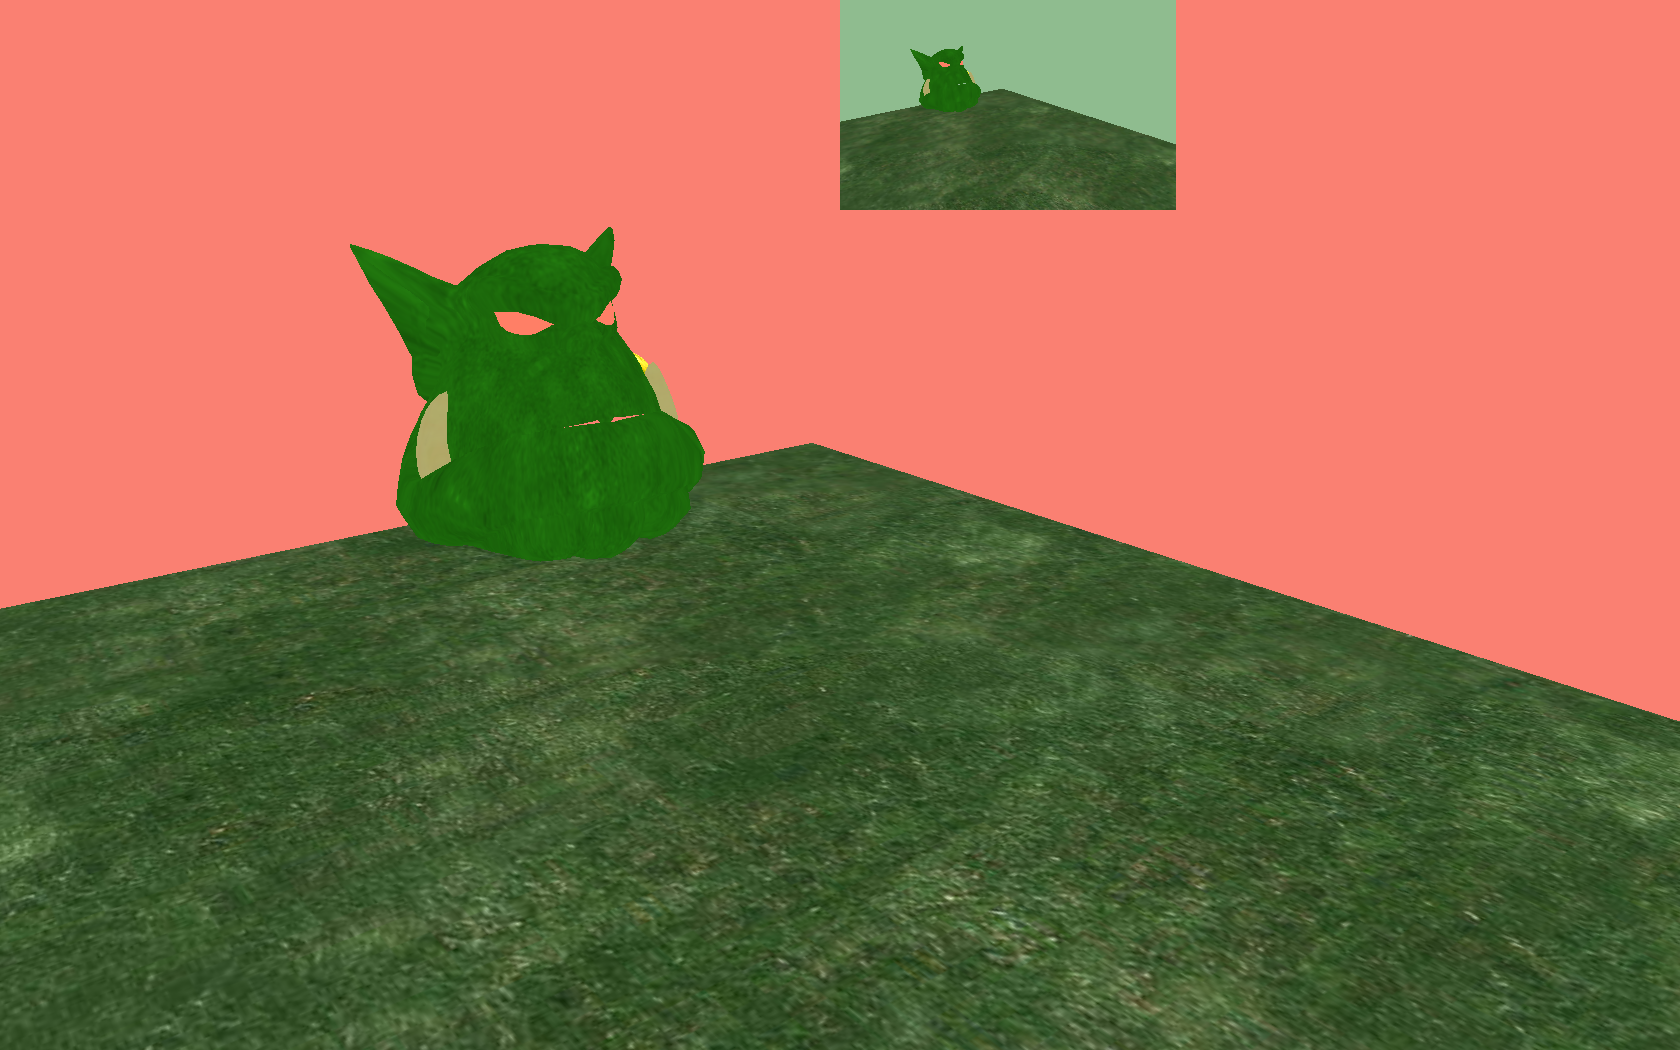
\includegraphics[scale=0.25]{Base_de_Ogre/Se_reperer_ds_l_espace/Images/plusieursViewport.png} 
	\end{center}






\subsubsection{Code: 3 vues}
Le code suivant permet la cr\'eation de deux viewports:


\begin{lstlisting}[caption={createViewports: cr\'eation de plusieurs vues}]



void PremiereApplication::createViewports()
{
    //Viewport "principal"
    Viewport *vue = mWindow->addViewport(mCamera);
    mCamera->setAspectRatio(Real(vue->getActualWidth()) /  Real(vue->getActualHeight()));
    vue->setBackgroundColour(ColourValue(0.980, 0.502, 0.447)); //saumon

	//seconde vue
    Viewport* vue2 = mWindow->addViewport(mCamera, 1, 0.5, 0, 0.8, 0.8);
    vue2->setBackgroundColour(ColourValue(0.561, 0.737, 0.561 ));  //darkseagreen

	//troisieme vue
	Viewport* vue3 = mWindow->addViewport(mCamera, 4, 0, 0.4, 0.2, 0.2);
    vue3->setBackgroundColour(ColourValue(0.878, 1.000, 1.000));  //
}
\end{lstlisting}

Et j'obtiens:
	\begin{center}
	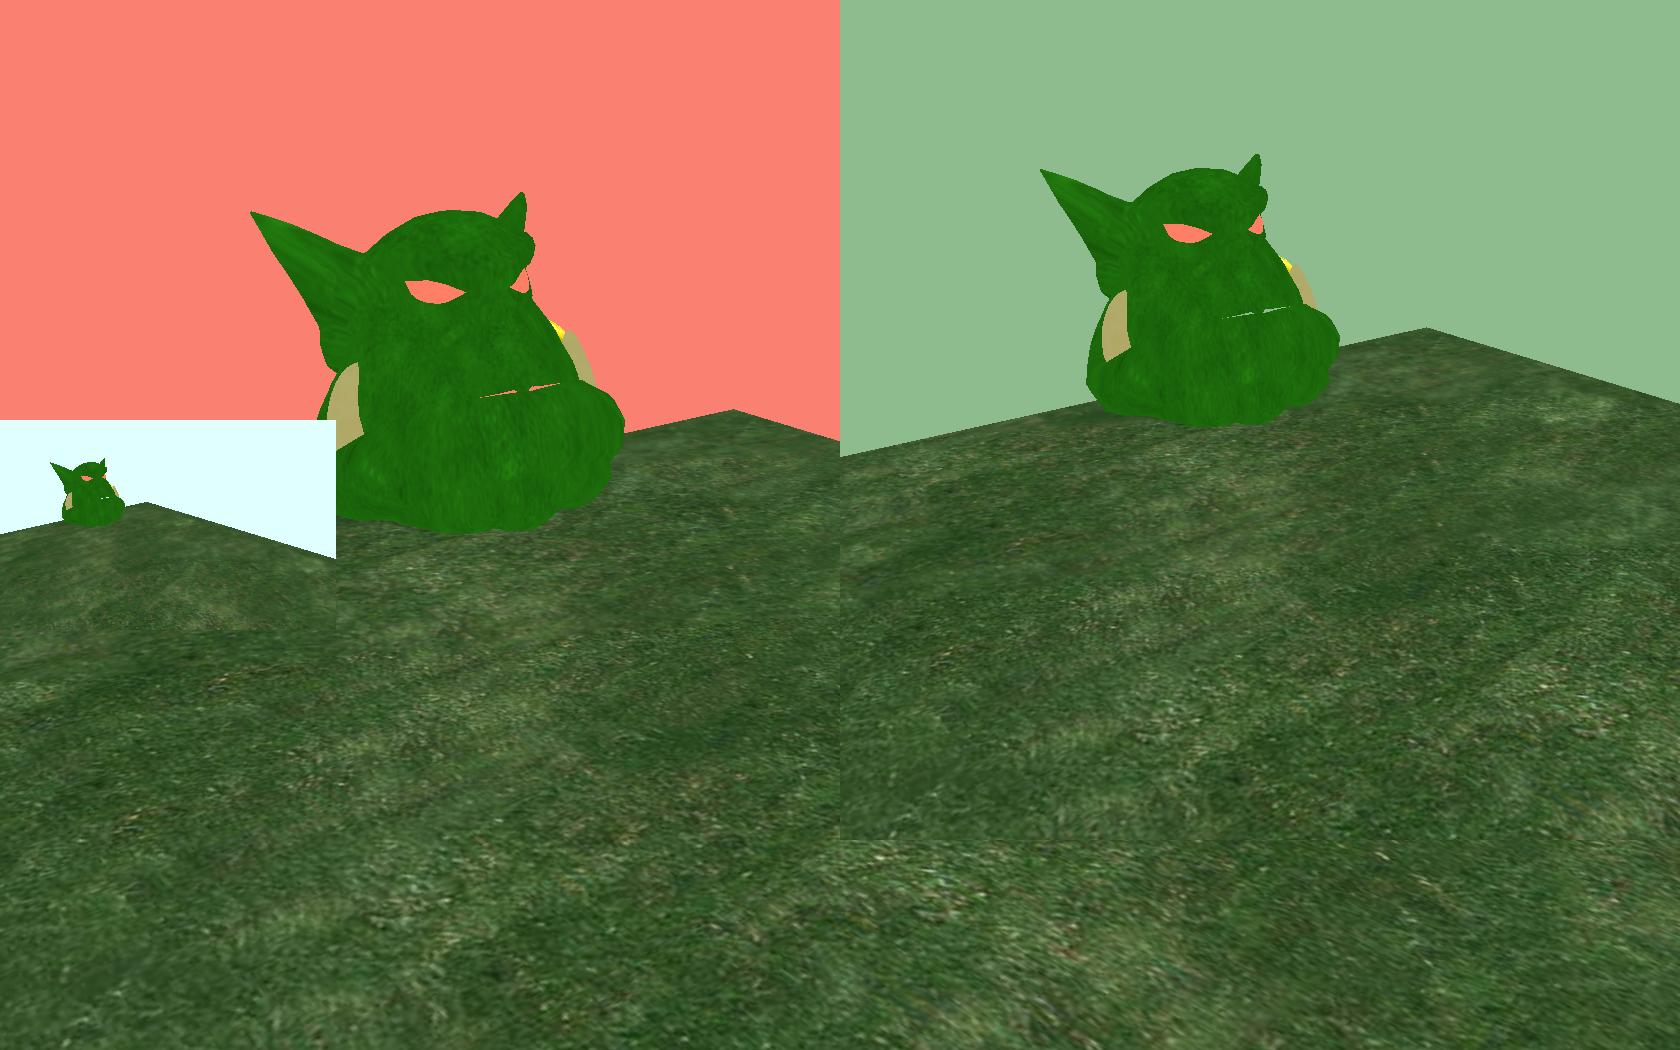
\includegraphics[scale=0.25]{Base_de_Ogre/Se_reperer_ds_l_espace/Images/plusieursViewport2.png} 
	\end{center}

























%---------------------------------------------------------------------------------------------------------------


\chapter{La lumières}



\section{Les lumières}


\subsection{Quelques fonctions de base}

La lumière est nécessaire pour pouvoir voir quelque chose dans une scène. Comment a-t-on donc pu voir nos objets depuis le début de ce cours?

Il existe une propriété du scène Manager qui permet de définir une lumière ambiante. Cela permet d'éclairer la scène de façon homogène avec une certaine luminosité. Par défaut, on a un éclairage à la lumière blanche qui permet de voir ce qui se passe dans la scène. La ligne suivante peut être ajoutée au début de la méthode createscene() pour appliquer une lumière ambiante noire nous pourrons ainsi définir des lumières et voir leur influence.

\begin{lstlisting}
msceneMgr->setAmbientLight(ColourValue(0.0, 0.0, 0.0));
\end{lstlisting}



La classe ColourValue permet de définir une couleur en entrant les quantités respectives de rouge, de vert puis de bleu dans un nombre compris entre 0 et 1. Il est aussi possible de définir une composante alpha (la transparence), utile pour des textures par exemple.

Une lumière est un objet de scène, on passe donc par le scène manager pour créer une lumière:
\begin{lstlisting}
Light *light = msceneMgr->createLight(''lumiere1'');
\end{lstlisting}

Par défaut, la lumière créée est de type ponctuelle. Vous avez plus de détails sur les différents types de lumière un peu plus bas.

Mettons tout de suite en place quelques paramètres de base: la couleur émise (diffuse et spéculaire, que nous détaillerons dans le chapitre sur les matériaux) et la position.
\begin{lstlisting}
light->setDiffuseColour(1.0, 0.7, 1.0);
light->setSpecularColour(1.0, 0.7, 1.0);
light->setPosition(-100, 200, 100);
\end{lstlisting}




Les deux premiers paramètres sont les couleurs diffuses et spéculaires, au format RVB, avec des valeurs qui doivent être comprises entre 0 et 1.

La couleur diffuse est la couleur sous laquelle vont apparaître les objets non brillants, et la couleur spéculaire est un paramètre supplémentaire pour les matériaux réfléchissants comme le métal ou le verre. Pour une lumière, on met généralement la même couleur pour ces deux paramètres.

Vient ensuite la méthode setPosition(), qui ne devrait pas vous poser de problèmes, et enfin une dernière ligne \footnote{quelle dernière ligne ???} permettant d'amplifier ou de diminuer l'intensité lumineuse. Par défaut, ce coefficient est de 1, mais pour notre scène j'ai voulu l'augmenter pour qu'on y voie un peu plus clair: n'hésitez pas à jouer un peu avec pour faire des essais.

Enfin, sachez qu'il est possible d'attacher une lumière à un noeud de scène. Dans ce cas, la méthode Light::setPosition() définit la position relative de la lumière par rapport au noeud.
\begin{lstlisting}
	node->attachObject(light);
\end{lstlisting}


Vous pouvez donc facilement placer une lumière à la position d'un mesh censé émettre de la lumière - par exemple les phares d'une voiture - et les déplacer en même temps grâce à une seule commande vers le noeud de scène!





\subsection{Les types de lumières}

Ogre peut gérer différents types de lumières selon l'effet désiré. Ils sont au nombre de 3:

\begin{itemize}
\item la lumière ponctuelle: cette lumière émet dans toutes les directions à partir de sa position;
\item la lumière directionnelle: une lumière dont les rayons vont dans une direction unique et qui n'a pas de position. C'est le genre de lumière qui permet de reproduire l'éclairage du soleil par exemple;
\item le projecteur ou spot: c'est une lumière qui émet un cône lumineux à partir de sa position, à la façon d'une lampe-torche.
\end{itemize}
    




\subsection{Lumière ponctuelle}
C'est le type de lumière créé par défaut que l'on a vu plus haut. Pour le modifier manuellement, il faut utiliser le type LT\_POINT.

\begin{lstlisting}
	light->setType(Light::LT_POINT);
\end{lstlisting}


Avec ce type de lumière, il existe une méthode nous permettant aussi de limiter la portée de notre éclairage. Voici le prototype:
\begin{lstlisting}
Light::setAttenuation( Real range, Real constant, Real linear, Real quadratic )
\end{lstlisting}



C'est plus délicat car les paramètres doivent être choisis avec soin. 
\begin{itemize}
\item Le premier est la distance caractéristique d'atténuation, c'est-à-dire la distance à partir de laquelle la luminosité diminue. 
\item constant est une constante d'atténuation comprise entre 0 et 1. Plus elle est proche de 0, et plus le passage de la lumière à l'ombre est brutal.
\item linear et quadratic sont les paramètres de la courbe d'atténuation, et doivent être assez faibles, sinon la lumière s'atténue trop rapidement.
\end{itemize}
	


Ça ne marche pas! L'ogre est bien éclairé mais le sol reste désespérément noir!

L'atténuation ajoute une caractéristique un peu différente pour la gestion de la lumière. En effet, l'éclairage des surfaces est calculé en fonction des vertices situés dans la zone d'éclairage. Lorsqu'un vertice est dans la zone d'éclairage du spot, la surface autour de lui est éclairée, sinon elle est dans l'ombre. Ogre se charge ensuite de faire les dégradés entre les vertices plus ou moins éclairés.

Mais ici, notre plan n'est constitué que de quatre vertices (les coins), dont aucun n'est éclairé par le spot. Le sol n'est donc pas éclairé.

Pour régler ça, il suffit de modifier notre sol pour qu'il possède plus de vertices. Retrouvez la définition du plan et modifiez les paramètres de découpage pour obtenir 10 segments en largeur et en longueur (les deux paramètres avant le true).

\begin{lstlisting}
Plane plan(Vector3::UNIT_Y, 0);
MeshManager::getSingleton().createPlane(''sol'', ResourceGroupManager::DEFAULT_RESOURCE_GROUP_NAME, plan, 500, 500, 10, 10, true, 1, 1, 1, Vector3::UNIT_Z);
\end{lstlisting}



Notez que plus il y aura de vertices sur le modèle, plus ce sera précis, mais ce sera un peu plus coûteux en ressources.




\subsection{Lumière directionnelle}

Étant donné que cette lumière est de type ''soleil'' et qu'elle émet à l'infini, il n'est pas utile de renseigner sa position. En revanche, la méthode setDirection() permet de définir le vecteur directeur des rayons lumineux.

\begin{lstlisting}
light->setType(Light::LT_DIRECTIONAL);
light->setDirection(10.0, -20.0, -5);
\end{lstlisting}






\subsection{Projecteur}

Le projecteur permet généralement de simuler un éclairage artificiel en proposant une lumière directionnelle définie dans un cône central et un cône extérieur, avec deux intensités différentes. Le cône central définit une lumière plus forte que le cône extérieur, où la lumière est quelque peu atténuée. Ces deux cônes sont définis par leur angle d'ouverture, ainsi que par un falloff, c'est-à-dire un coefficient indiquant si la transition entre les deux cônes doit être plus ou moins rapide:
\begin{lstlisting}
light->setType(Light::LT_SPOTLIGHT);
light->setPosition(0, 150, -100);
light->setDirection(0, -1, 1);
light->setSpotlightRange(Degree(30), Degree(60), 1.0);
\end{lstlisting}


Notez que l'éclairage du spot obéit aux mêmes règles que pour l'atténuation d'une lumière ponctuelle: il faut que les vertices soient éclairés pour que l'éclairage soit visible.


De même que pour les lumières ponctuelles, vous pouvez ajouter une portée limitée à votre projecteur avec la méthode setAttenuation().






\section{Les ombres}


\subsection{Activer les ombres}

Tout d'abord, on doit paramétrer nos lumières et nos entités pour projeter (ou non) des ombres.
Que ce soit pour les lumières ou les entités, on utilise la même méthode pour choisir d'activer ou non la projection:

\begin{lstlisting}
light->setCastShadows(true);
head->setCastShadows(true);
\end{lstlisting}


Si vous voulez qu'une entité ne projette aucune ombre, il suffit de mettre le paramètre à false. De même si vous voulez qu'une lumière ne projette aucune ombre pour les entités (pour une lumière d'ambiance ou d'ajustement, par exemple).

N'oubliez pas de désactiver la projection d'ombres pour le sol. D'une part parce que celui-ci n'a pas besoin de projeter d'ombres, d'autre part parce que certaines techniques nécessitent d'avoir ce paramètre désactivé pour avoir une ombre sur le mesh.

Avant de pouvoir afficher les ombres, il faut les activer. Cela se fait dans le scène Manager, par exemple:

\begin{lstlisting}
msceneMgr->setShadowTechnique(Ogre::SHADOWTYPE_STENCIL_ADDITIVE);
\end{lstlisting}



On définit ici la technique de rendu qui sera utilisée pour les ombres dans la scène (voir ci-dessous).




\subsection{Les différents types d'ombres}

Ogre permet de générer différents types d'ombres selon les besoins, qui dépendent généralement des modèles concernés par la projection d'ombres.

Il existe deux techniques pour la génération d'ombres:
\begin{itemize}
\item le type ''Stencil'' (pochoir en anglais)
\item le type ''Texture''
\end{itemize}

Les ombres de type Stencil sont très précises dans les contours et permettent une très bonne projection d'ombre lorsque l'on y regarde de près. En revanche, elles sont assez coûteuses en ressources, notamment lorsque les mesh sont animés. Enfin, elles ne prennent pas du tout en compte la transparence des textures, un cube de texture transparente projettera donc une ombre si ce paramètre est activé.
Les ombres de type Texture permettent de gérer la transparence des textures et sont moins coûteuses en ressources, mais leur précision est plus faible.

Enfin, chacune de ces deux catégories est composée de deux techniques, l'une dite modulative, l'autre additive. On obtient ainsi quatre techniques possibles:
\begin{itemize}
\item SHADOWTYPE\_TEXTURE\_MODULATIVE
\item SHADOWTYPE\_TEXTURE\_ADDITIVE
\item SHADOWTYPE\_STENCIL\_MODULATIVE
\item SHADOWTYPE\_STENCIL\_ADDITIVE
\end{itemize}


Notez que dans chacun des cas, la technique additive est la meilleure, notamment pour une approche de type Stencil. La différence pour les techniques de type Texture est minime; en revanche, la technique Stencil additive permet d'obtenir des ombres plus ou moins sombres en fonction de l'éclairage grâce à des passes successives, tandis que la méthode Stencil modulative ne fait que projeter le modèle au sol une seule fois pour chaque lumière.

C'est donc dans le scène Manager que l'on s'occupe de déterminer la technique de rendu des ombres. Par défaut, celles-ci ne sont pas rendues.
\begin{lstlisting}
msceneMgr->setShadowTechnique(Ogre::SHADOWTYPE_STENCIL_MODULATIVE);
\end{lstlisting}


Il n'est possible d'avoir qu'une seule technique enregistrée à la fois dans un scène Manager. Il n'est pas possible de choisir les types d'ombres à générer pour chaque lumière de la scène. Il faut donc faire un choix pour l'ensemble de vos ombres.

Ci-dessous, l'approche basée sur la texture, peu précise mais peu coûteuse en ressources:

Image utilisateur \url{http://fr.openclassrooms.com/informatique/cours/decouvrez-ogre-3d/les-ombres-1}



\subsection{Code}
Dans le code ci-dessous a été ajoutée une méthode pour la création d'une lumière et les ombres. Les objets qui projettent des ombres doivent être activé, ici seule la tête de ogre et la lumière elle-même projettent des ombres.

\subsubsection{PremiereApplication.h}



\begin{lstlisting}[caption={PremiereApplication.h: ajout d'une méthode pour la gestion de lumière et des ombres}]
using namespace std;

#include <ExampleApplication.h>
#include <OgreMovableObject.h>


class PremiereApplication : public ExampleApplication
{
    public:
        void createScene();
        void createCamera();
        void createViewports();

        void createLux(std::string, MovableObject *);
};

\end{lstlisting}







\subsubsection{PremiereApplication.cpp}



\begin{lstlisting}[caption={PremiereApplication.cpp: ajout d'une méthode pour la gestion de lumière et des ombres}]
#include "PremiereApplication.h"

void PremiereApplication::createScene()
{
    //creation d une entite
    Entity *head= mSceneMgr->createEntity("Tete", "ogrehead.mesh" );
    
    //creation d un noeud
    SceneNode *node= mSceneMgr->getRootSceneNode( )->createChildSceneNode( "nodeTete " , Vector3::ZERO, Quaternion::IDENTITY);
    
    node->yaw(Radian(Math::PI));
    node->yaw(Radian(Math::PI));

    //setPosition place le noeud aux coord passees en parametres
    Vector3 position = Vector3(30.0, 50.0, 0.0);
    node->setPosition(position);

    node->setPosition(30.0, 50.0, 0.0); 
    /*equivalent a
    Vector3 position = Vector3(30.0, 50.0, 0.0);
    node->setPosition(position);
    */

    //deplace le noeud par rapport a sa position actuelle
    node->translate(-30.0, 50.0, 0.0); //par defaut la trnslt se fait par rap a TS_WORLD
   
    //attachement de l entite au noeud
    node->attachObject(head);

    //creation d un plan
    Plane plan(Vector3::UNIT_Y, 0);

    //creation d un mesh cad l objet 3d visible ds la scene
    MeshManager::getSingleton().createPlane("sol",  ResourceGroupManager::DEFAULT_RESOURCE_GROUP_NAME, plan, 500, 500, 10, 10, true, 1, 1, 1, Vector3::UNIT_Z); 

    //entite qui representera le plan
    Entity *ent= mSceneMgr->createEntity("EntiteSol", "sol");

    //ajout du materiau a l entite
    ent->setMaterialName("Examples/GrassFloor");//texture de pelouse
    /*les differents materiaux sont sous /media/materials/scritps, par ex:
    ent->setMaterialName("Examples/WaterStream");//texture d eau animee*/

    //creation d un noeud
    node = mSceneMgr->getRootSceneNode()->createChildSceneNode();
    node->attachObject(ent);

    createLux("ponctuelle", head);//lumiere ponctuelle
    //createLux("directionnelle", head);//lumiere directionnelle
    //createLux("spot", head);//lumiere projecteur
}

/*
cree une lumiere selon le parametre passe:
    createLux("ponctuelle"); -> lumiere ponctuelle
    createLux("directionnelle"); -> lumiere directionnelle
    createLux("spot"); -> lumiere projecteur
    
    le second parametre est l entite pour laquelle on active les ombres

une lumiere noire est cree au debut de la methode

une ombre est cree en fin de methode
*/
void PremiereApplication::createLux(std::string prmLightType, MovableObject * prmEnt)
{
    //application d une couleur noire
    mSceneMgr->setAmbientLight(ColourValue(0.0, 0.0, 0.0)); 

    //definition d une lumiere 
    Light *light= mSceneMgr->createLight("lumiere1");

    if (prmLightType == "ponctuelle")
    {
        //definition du type de lumiere
        light->setType(Light::LT_POINT);//lumiere ponctuelle

        //definition de la position de la lumiere
        light->setPosition(-100, 200, 100);
    }
    else if (prmLightType == "directionnelle")
    {
        light->setType(Light::LT_DIRECTIONAL);//lumiere directionnelle
        light->setDirection(10.0, -20.0, -5);//vecteur directeur de la lumiere directionnelle

        //definition de la position de la lumiere
        light->setPosition(-100, 200, 100);
    }
    else
    {
        light->setType(Light::LT_SPOTLIGHT);//lumiere directionnelle
        light->setDirection(0.0, -1, 1);//vecteur directeur de la lumiere directionnelle
        light->setSpotlightRange(Degree(30), Degree(60), 1.0);
    }

    //definition des couleur des lumieres diffuse
    light->setDiffuseColour(1.0, 0.7, 0.1);
    //et speculaire
    light->setSpecularColour(1.0, 0.7, 0.1);

    //ombre
    //activation de la projection des ombres
    light->setCastShadows(true);
    prmEnt->setCastShadows(true);

    //activation des ombres
    mSceneMgr->setShadowTechnique(Ogre::SHADOWTYPE_STENCIL_ADDITIVE);

}

/*definit la position de notre point de vue*/
void PremiereApplication::createCamera()
{
    //creation de la camera
    mCamera = mSceneMgr->createCamera("Ma Camera");

    //position de la camera
    mCamera->setPosition(Vector3(-100.0, 150.0, 200.0));

    //permet de determiner le point de la scene que regarde notre camera
    mCamera->lookAt(Vector3(0.0, 100.0, 0.0));

    //definition des distances de near clip et de far clip, qui
    //sont les distances minimale et maximale auxquelles doit se
    //trouver un objet pour etre afficher a l ecran.
    mCamera->setNearClipDistance(1);
    mCamera->setFarClipDistance(1000);
}

void PremiereApplication::createViewports()
{
    //la creation du Viewport, appelee par la fenetre et prenant en parametre la
    //camera concernee, le premier parametre est la camera de laqll le contenu
    //du viewport sera rendu, ce paramatre est le seul obligatoire
    Viewport *vue = mWindow->addViewport(mCamera);
    //Viewport *vue = mWindow->addViewport(mCamera, 0, 0, 0, 0.8, 0.8);

    //Grace a ce Viewport nouvellement cree, nous allons faire coincider
    //le rapport largeur / hauteur de notre camera avec celui du
    //Viewport, pour avoir une image non deformee
    mCamera->setAspectRatio(Real(vue->getActualWidth()) /  Real(vue->getActualHeight()));

    //on definit ici la couleur de fond
    //vue->setBackgroundColour(ColourValue(0.0, 0.0, 1.0));     //bleu
    vue->setBackgroundColour(ColourValue(0.980, 0.502, 0.447)); //saumon

   // creation d'un viewport dans le coin bas gauche
   //les parametres autres que le premier sont obligatoires pour la definition
   //de plusieurs viewport
   Viewport* vue2 = mWindow->addViewport(mCamera, 1, 0, 0.8, 0.2, 0.2);
   vue2->setBackgroundColour(ColourValue(0.561, 0.737, 0.561 ));  //darkseagreen
}


\end{lstlisting}





%---------------------------------------------------------------------------------------------------------------
\chapter{La gestion des entr\'ees}




\section{Les frame listeners}





\subsection{Des ''\'ecouteurs d'images'' ?}
\subsubsection{Utilit\'e}
Lorsque vous g\'erez les entr\'ees de l'utilisateur (et m\^eme pour faire des calculs divers durant l'ex\' ecution de votre programme), l'ordinateur effectue les instructions n\'ecessaires entre deux images (ou frames en anglais), donc pendant un temps tr\`es court.

En pratique, le moteur fonctionne dans une boucle, qui ne fait qu'afficher une image, puis fait des calculs; et ainsi de suite, sans s'arr\^eter. Il est donc possible pour le programmeur de donner ses instructions avant qu'une image soit rendue, ou bien apr\`es, ou bien m\^eme pendant que la carte graphique fait le rendu graphique.

Lorsque l'on aura vu comment cr\'eer cette boucle de rendu, nous serons \`{a} m\^eme de donner les instructions de la mani\`ere dont nous le d\'esirons. En attendant, je vais vous pr\'esenter une classe qui a l'avantage de permettre de faire tout ce que je viens de vous expliquer de fa\c{c}on tr\`es simple: le frame listener.



\subsubsection{Les m\'ethodes \`{a} conna\^itre}
Un frame listener est une classe interface qui poss\`ede trois m\'ethodes, dont voici les prototypes:

\begin{itemize}
\item virtual bool frameStarted(const FrameEvent\& evt): est appel\'ee avant que la frame ne soit rendue (frameStarted)
\item virtual bool frameRenderingQueued(const FrameEvent\& evt): est appel\'ee apr\`es que la frame ait \'et\'e rendue (frameEnded)
\item virtual bool frameEnded(const FrameEvent\& evt): est appel\'ee apr\`es que le processeur graphique ait re\c{c}u les instructions pour le rendu (frameRenderingQueued)\newline
\end{itemize}
    


En cr\'eant un objet d\'eriv\'e de la classe frame listener dans votre application et en r\'eimpl\'ementant ces m\'ethodes virtuelles, vous avez donc la possibilit\'e de demander \`{a} Ogre d'effectuer les calculs dont vous avez besoin \`{a} chaque image.



frameStarted() et frameEnded() sont tr\`es similaires, \'etant donn\'e qu'elles ont pour seule diff\'erence d'\^etre appel\'ees respectivement au d\'ebut et \`{a} la fin de la boucle de rendu. Mais comme on est dans une boucle, en r\'ealit\'e il ne se passe quasiment rien entre l'appel \`{a} frameEnded() et celui \`{a} frameStarted(). La diff\'erence peut \^etre utile par exemple si vous avez un calcul qui semble plus logique d'effectuer apr\`es que l'image soit rendue plut\^ot qu'avant, mais ce n'est qu'une question de lecture du code selon moi.


En revanche la derni\`ere (frameRenderingQueued) est plus subtile. Comme je l'ai dit, elle est appel\'ee d\`es que la carte graphique re\c{c}oit les instructions n\'ecessaires pour afficher l'image \`{a} rendre.


Vous le savez probablement, c'est une op\'eration tr\`es co\^uteuse en ressources et c'est souvent ce qui ralentit les jeux vid\'eo mettant en jeu de nombreux effets graphiques. Pendant ce temps-l\`{a}, le processeur central attend que \c{c}a se passe. Par cons\'equent, si vous appelez la m\'ethode frameRenderingQueued() pour faire des calculs, vous \'evitez d'avoir un processeur peu occup\'e pendant que la carte graphique fait son boulot !

De mani\`ere g\'en\'erale, on pourra utiliser cette m\'ethode pour des op\'erations lourdes dont on sait qu'elles seront r\'ep\'et\'ees \`{a} chaque image, afin de rentabiliser l'utilisation du processeur.




\subsubsection{Contr\^ole de l'ex\'ecution}

La valeur de retour des m\'ethodes d'un frame listener est un bool\'een r\'ecup\'er\'e par Ogre pour savoir s'il doit continuer (true) ou non (false) l'ex\'ecution du programme.



\subsubsection{Utiliser plusieurs frame listeners}

Il est possible de cr\'eer autant de frame listeners que vous le d\'esirez, pour effectuer des op\'erations diverses. En revanche, il est conseill\'e de ne pas en abuser pour \'eviter de trop segmenter votre application, il peut \^etre int\'eressant d'appeler d'autres fonctions \`{a} partir d'un frame listener plut\^ot que d'en cr\'eer trop.

Enfin, et c'est l\`{a} le plus important:
\textbf{L'ordre d'ex\'ecution des frame listeners est laiss\'e aux soins du moteur. Vous n'avez AUCUN contr\^ole dessus !}

En d'autres termes, si vous avez besoin d'effectuer des op\'erations dans un ordre pr\'ecis, ne les mettez pas dans des frame listeners diff\'erents, car vous ne pourrez pas d\'ecider de l'ordre d'ex\'ecution. Il faut alors laisser un seul frame listener g\'erer les op\'erations, ou ne pas passer par eux (ce sera possible lorsque nous attaquerons la boucle de rendu).



\subsection{Le frame listener en pratique}

Comme nous allons vouloir red\'efinir les m\'ethodes du frame listener, il faut en faire une classe d\'eriv\'ee. Vu que nous sommes dans la gestion des entr\'ees, nous allons tout de suite pr\'eparer le terrain en cr\'eant une classe InputListener d\'erivant de ExampleFrameListener.

Je d\'erive ici de la classe ExampleFrameListener, elle-m\^eme d\'eriv\'ee de FrameListener, car la classe ExampleApplication met d\'ej\`{a} en place une gestion des entr\'ees et attend un ExampleFrameListener. Cette classe s'occupe aussi de construire les objets n\'ecessaires \`{a} l'\'ecoute des entr\'ees souris/clavier, ce que nous aborderons ult\'erieurement.
Cependant, la m\'ethode de traitement reste identique, nous allons juste devoir red\'efinir frameRenderingQueued() pour impl\'ementer notre propre gestion des entr\'ees \`{a} la place de celle pr\'evue par ExampleFrameListener.


\begin{lstlisting}[caption={InputListener.h}]
#include ''ExampleFrameListener.h''
class InputListener: public ExampleFrameListener
{
public:
    InputListener(RenderWindow* win, Camera* cam, sceneManager *sceneMgr, bool bufferedKeys = false, bool bufferedMouse = false, bool bufferedJoy = false );
    virtual bool frameRenderingQueued(const FrameEvent& evt);

private:
    Ogre::sceneManager *msceneMgr; //pointeur sur le scene Manager, qui servira a retrouver des objets dans la scene.
    bool mToucheAppuyee;	 //pour garder une trace de l etat dans lequel se trouve une touche particuliere.

    /*distance de deplacement de la camera et sa vitesse, puis des angles de rotation.*/
    Ogre::Real mMouvement;
    Ogre::Real mVitesse;
    Ogre::Real mVitesseRotation;

	/*angles de rotation.*/
    Ogre::Radian mRotationX;
    Ogre::Radian mRotationY;
};
\end{lstlisting}



Dans votre fichier InputListener.cpp, pr\'eparez le constructeur ainsi que l'impl\'ementation des m\'ethodes, avec un corps vide pour l'instant:

%je ne sais pas si [language=cpp] passe et s il est utile
\begin{lstlisting}[caption={InputListener.cpp}]
/*
Arguments:
RenderWindow* win: votre RenderWindow pour l'application
Camera* cam: la camera que vous utilisez
sceneManager *sceneMgr: le scene Manager
bool bufferedKeys: indique si vous desirez utiliser le buffer pour le clavier
bool bufferedMouse: indique si vous desirez utiliser le buffer pour la souris
bool bufferedJoy: indique si vous desirez utiliser le buffer pour le joystick
*/
InputListener::InputListener(RenderWindow* win, Camera* cam, sceneManager *sceneMgr, bool bufferedKeys, bool bufferedMouse, bool bufferedJoy) 
      : ExampleFrameListener(win, cam, bufferedKeys, bufferedMouse, bufferedJoy)
{
    msceneMgr = sceneMgr;
    mVitesse = 100;
    mVitesseRotation = 0.3;
    mToucheAppuyee = false;
}
\end{lstlisting}



Il n'y a pas de constructeur \'ecrit pour les frame listeners, car c'est une classe interface\footnote{que je sache il n'y a pas d'interface en C++}\footnote{pas de constructeur parce que c'est une classe interface ??}, seules les trois m\'ethodes que j'ai pr\'esent\'ees plus haut importent. En revanche, la classe ExampleFrameListener poss\`ede un constructeur qui pr\'epare le terrain pour l'utilisation des entr\'ees, que j'appelle dans ma classe d\'eriv\'ee. 

Les trois bool\'eens en param\`etres indiquent si vous d\'esirez utiliser le buffer respectivement pour le clavier, la souris et le joystick. Comme ce sera l'objet de la derni\`ere partie de ce chapitre, je mets par d\'efaut false (dans le .h).

Dans le corps du constructeur, j'initialise mes attributs mSceneMgr, mVitesse et mToucheAppuyee, qui nous serviront par la suite.

Il n'y a pas d'attribut \`{a} ajouter dans notre classe PremiereApplication, la classe ExampleApplication contient d\'ej\`{a} un pointeur sur un ExampleFrameListener.

       




































\section{OIS}


Pour g\'erer les entr\'ees de l'utilisateur, nous allons utiliser la biblioth\`eque OIS \footnote{Object Oriented Input System, c'est \`a dire: Syst\`eme d'entr\'ees orient\'e objet}, qui est distribu\'ee par d\'efaut avec le SDK d'Ogre. Comme je l'ai dit en introduction de ce cours, un moteur 3D n'a pas de m\'ethodes pour g\'erer autre chose que ce qui s'affiche sur votre \'ecran. C'est pourquoi nous utiliserons cette biblioth\`eque pour r\'ecup\'erer les actions du joueur.\newline


Pour ce faire, OIS repr\'esente les p\'eriph\'eriques d'entr\'ee par des objets, qui sont les suivants:

\begin{itemize}
\item Mouse pour la souris;
\item Keyboard pour le clavier;
\item Joystick pour les joysticks ou manettes de jeu.\newline
\end{itemize}
    



Qui dit nouvelle biblioth\`eque dit nouveau namespace ! Ces classes se trouvent donc dans l'espace de nom OIS.\newline

Les touches du clavier et les boutons de la souris sont des \'enum\'erations, d\'efinies comme ceci:

\begin{itemize}
\item OIS::KC\_NOMDELATOUCHE pour le clavier;
\item OIS::MB\_NOMDUBOUTON pour la souris.
\end{itemize}


Ce qui donne par exemple OIS::KC\_A pour la touche 'A'\footnote{la touche 'Entr\'ee' s'appelle 'Return' en anglais, ne cherchez donc pas OIS::KC\_ENTER, vous ne trouverez pas.}, ou OIS::MC\_Left pour le clic gauche.\newline

Une derni\`ere chose bonne \`{a} savoir: les codes de touches d'OIS correspondent aux touches physiques d'un clavier QWERTY. Ce qui signifie par exemple que OIS::KC\_A correspond \`{a} la touche Q sur votre clavier AZERTY.\newline

Afin d'utiliser OIS, il faut inclure le header correspondant. Celui-ci se trouve dans le dossier OIS du dossier include, on ajoutera donc la ligne de pr\'eprocesseur suivante en t\^ete du header de InputListener:

\begin{lstlisting}[caption={Include OIS}]
#include <OIS/OIS.h>
\end{lstlisting}

Bien s\^ur, vous pouvez aussi ajouter le r\'epertoire OIS \`{a} la liste des includes de votre IDE pour \'eviter d'avoir \`{a} le pr\'eciser dans le code.




























\section{Allons-y sans buffer}\footnote{Le tutorial du site de Ogre ''Frame Listeners and Unbuffered Input'' pr\'esente le point trait\'e ici d'une autre mani\`ere \href{http://www.ogre3d.org/tikiwiki/Basic+Tutorial+4}{Frame Listeners and Unbuffered Input}}
\subsection{Explications}
Dans le constructeur de notre frame listener, je vous ai dit que l'on avait mis les param\`etres concernant l'utilisation du buffer \`a false, car c'est l'objet de la derni\`ere partie de ce chapitre. Mais que signifie le fait d'utiliser ou non le buffer ?

Lorsque vous appuyez sur une touche, le clavier envoie un signal \`a l'ordinateur pour lui dire qu'une touche est actuellement press\'ee, en pr\'ecisant quelle touche est concern\'ee. Ce signal est envoy\'e tant que la touche reste enfonc\'ee.

De son cot\'e, notre programme effectue sa boucle infinie, rendant les images et faisant les calculs demand\'es. Supposons que vous appuyez sur une touche \`a un instant donn\'e. Lorsque l'ordinateur arrivera \`a l'instruction lui demandant de regarder ce qui se passe sur le clavier, il va voir qu'une touche est enfonc\'ee et cherchera \`a effectuer les op\'erations demand\'ees, et ceci tant que la touche reste enfonc\'ee. Mais il n'est pas possible pour l'ordinateur de faire seul la diff\'erence entre une touche enfonc\'ee et une touche qui vient d'\^etre enfonc\'ee.

Nous allons donc voir comment r\'egler ce probl\`eme ''\`a la main'', puis nous verrons l'utilisation du buffer, qui constitue une autre fa\c{c}on de traiter l'entr\'ee.

\subsection{Cr\'eation du frame listener}

Avant de passer \`a la suite, r\'eimpl\'ementez la m\'ethode createFrameListener() pr\'esente dans ExampleApplication dans la classe PremiereApplication en ajoutant le prototype et la d\'efinition :

\begin{lstlisting}[caption={PremiereApplication::createFrameListener}]
void PremiereApplication::createFrameListener()
{
    //creation du framelistener en utilisant le ctor prepare plus tot
    mFrameListener= new InputListener(mWindow, mCamera, mSceneMgr, false, false, false);
    //signale a l objet root que ns avons un nv frame listener et qu il faudra l'appeler
    mRoot->addFrameListener(mFrameListener);
}
\end{lstlisting}

Le root est l'\'el\'ement de base de l'application Ogre qui s'occupe notamment de g\'erer les frame listeners, nous le reverrons plus tard en approfondissant le fonctionnement du moteur.
 









\subsection{D\'eplacer la cam\'era}


Tout d'abord, nous allons consid\'erer le d\'eplacement de cam\'era, pour lequel nous n'avons pas besoin de savoir si la touche vient d'\^etre appuy\'ee : c'est simplement son \'etat actuel qui compte.

Premi\`erement, il nous faut r\'ecup\'erer l'\'etat actuel du clavier et de la souris. Localisez la m\'ethode frameRenderingQueued() de votre InputListener et ins\'erez-y ceci :


\begin{lstlisting}[caption={}]
if(mMouse)
    mMouse->capture();
if(mKeyboard)
    mKeyboard->capture();
\end{lstlisting}

Ces deux lignes permettent de mettre \`a jour nos objets pour obtenir le nom des touches enfonc\'ees.\newline

V\'erifions d'abord si la touche Echap est utilis\'ee, auquel cas nous quitterons l'application.


\begin{lstlisting}[caption={}]
if(mKeyboard->isKeyDown(OIS::KC_ESCAPE))
    return false;
\end{lstlisting}

Nous devons ensuite mettre \`a jour la valeur de mMouvement, qui sera la distance parcourue par la cam\'era si une direction est choisie. Comme le nombre d'images par seconde est variable, nous utilisons la propri\'et\'e timeSinceLastFrame de l'\'ev\'enement, multipli\'ee par la vitesse de la cam\'era. Le produit de la vitesse par le temps \'ecoul\'e nous donne donc la distance parcourue.

J'ai aussi cr\'e\'e un vecteur dans lequel nous allons enregistrer les d\'eplacements \`a effectuer. En effet, on peut utiliser plusieurs touches en m\^eme temps, il faut donc additionner les directions demand\'ees, et les conserver pour d\'eplacer la cam\'era en une seule fois.


\begin{lstlisting}[caption={}]
Ogre::Vector3 deplacement = Ogre::Vector3::ZERO;
mMouvement = mVitesse * evt.timeSinceLastFrame;
\end{lstlisting}

Nous allons utiliser les fl\`eches du clavier et les touches Z, S, Q, D pour nous d\'eplacer ; j'ai aussi impl\'ement\'e les touches fl\'ech\'ees, qui sont une configuration alternative pour le d\'eplacement. Il faut donc v\'erifier si les touches qui nous int\'eressent sont enfonc\'ees :


\begin{lstlisting}[caption={}]
// La touche A d'un clavier QWERTY correspond au Q sur un AZERTY
if(mKeyboard->isKeyDown(OIS::KC_LEFT) || mKeyboard->isKeyDown(OIS::KC_A)) 
    deplacement.x -= mMouvement;

if(mKeyboard->isKeyDown(OIS::KC_RIGHT) || mKeyboard->isKeyDown(OIS::KC_D))
    deplacement.x += mMouvement;
    
// W correspond au Z du AZERTY
if(mKeyboard->isKeyDown(OIS::KC_UP) || mKeyboard->isKeyDown(OIS::KC_W)) 
    deplacement.z -= mMouvement;

if(mKeyboard->isKeyDown(OIS::KC_DOWN) || mKeyboard->isKeyDown(OIS::KC_S))
    deplacement.z += mMouvement;
\end{lstlisting}

Attention aux signes ! Vous devez respecter ce que nous avons vu dans le chapitre sur les d\'eplacements !\footnote{hein? de quoi parle t il?}

Le d\'eplacement de la cam\'era fonctionne, il ne manque plus que la rotation de celle-ci. Il nous suffit pour cela de r\'ecup\'erer le d\'eplacement relatif depuis la derni\`ere fois que la souris a boug\'e (depuis le dernier appel \`a frameRenderingQueued() donc).

Pour retrouver cette valeur, on passe successivement par les attributs suivants :
\begin{itemize}
\item le mouseState contenu dans l'objet souris, contenant diverses informations sur l'\'etat de la souris ;
\item l'axe que l'on d\'esire observer : ici, ce sera X ou Y pour le yaw ou le pitch ;
\item le d\'eplacement relatif de la souris suivant cet axe.
\end{itemize}

Maintenant, occupons-nous du mouvement de la souris. Pour r\'ecup\'erer le d\'eplacement de celle-ci, nous devons r\'ecup\'erer son \'etat, comme indiqu\'e dans le code suivant.


\begin{lstlisting}[caption={}]
const OIS::MouseState &mouseState = mMouse->getMouseState();
\end{lstlisting}

\`A partir de cette r\'ef\'erence on peut notamment r\'ecup\'erer le d\'eplacement de la souris depuis la derni\`ere image, en appelant l'axe X ou Y puis l'attribut rel.


\begin{lstlisting}[caption={}]
mRotationX = Degree(-mouseState.Y.rel * mVitesseRotation);
mRotationY = Degree(-mouseState.X.rel * mVitesseRotation);
\end{lstlisting}

Il faut particuli\`erement faire attention aux axes et aux signes. Je consid\`ere que mRotationX (respectivement mRotationY) correspond \`a la rotation autour de l'axe X (respectivement Y), c'est-\`a-dire lorsque je d\'eplace ma souris en avant ou en arri\`ere (respectivement \`a gauche ou \`a droite). Or, le d\'eplacement vers l'avant ou l'arri\`ere de la souris correspond \`a son axe Y, c'est pour \c{c}a que je demande l'axe Y de la souris pour trouver la rotation autour de X dans l'espace 3D.

On rajoute une multiplication par la vitesse de rotation voulue et on convertit le tout en degr\'es, sinon le mouvement est bien trop rapide.

Enfin, on appelle les m\'ethodes de rotation et de d\'eplacement de la cam\'era :

\begin{lstlisting}[caption={}]
mCamera->yaw(mRotationY);
mCamera->pitch(mRotationX);
mCamera->moveRelative(deplacement);
\end{lstlisting}

La derni\`ere ligne, comme vous le remarquez, d\'eplace la cam\'era par rapport \`a son rep\`ere local, ce qui \'evite de faire la transformation de la variable deplacement \`a la main. Il est aussi possible de demander un d\'eplacement par rapport au rep\`ere absolu avec Camera::move().


















\subsection{Et avec un noeud de sc\`ene ?}

J'en profite pour vous montrer comment on aurait proc\'ed\'e pour d\'eplacer un noeud de sc\`ene par exemple, qui utilise la m\'ethode translate().

Les deux lignes suivantes sont \'equivalentes :


\begin{lstlisting}[caption={}]
node->translate(deplacement, TS_LOCAL);
node->translate(node->getOrientation() * deplacement, TS_PARENT);
\end{lstlisting}


La premi\`ere ligne est tr\`es similaire \`a celle utilis\'ee pour la cam\'era, il suffit de pr\'eciser que l'on se d\'eplace par rapport au rep\`ere local du noeud de sc\`ene.

La seconde solution indique un d\'eplacement relatif au noeud parent, mais utilise le quaternion retourn\'e par la m\'ethode getOrientation() multipli\'e par le vecteur de d\'eplacement pour obtenir la direction souhait\'ee dans ce rep\`ere. En pratique, on utilisera seulement la premi\`ere ligne, plus courte et plus propre dans le code.







\subsection{}
Mini-TP : cr\'eer un interrupteur

Pour g\'erer un \'ev\'enement qui ne doit arriver qu'une fois lorsque la touche est appuy\'ee, il y a une pr\'ecaution suppl\'ementaire \`a prendre. Je vous ai dit plus haut que votre ordinateur ne retenait pas l'\'etat dans lequel se trouvait votre clavier ou votre souris \`a l'image pr\'ec\'edente. Cependant, rien ne nous emp\^eche de le faire nous-m\^emes !

\`A titre d'exemple, disons que l'on veut utiliser la touche T pour allumer et \'eteindre la lumi\`ere de notre sc\`ene. Il va donc falloir v\'erifier \`a chaque image si la touche T est enfonc\'ee, et si en plus ce n'\'etait pas d\'ej\`a le cas \`a l'image pr\'ec\'edente. Pour cela, on utilisera l'attribut mToucheAppuyee de notre classe InputListener.

Un indice: le SceneManager poss\`ede une m\'ethode getLight() qui permet de r\'ecup\'erer un pointeur sur une lumi\`ere \`a partir du nom de celle-ci...

\`A vos claviers ! La r\'eponse se trouve juste apr\`es.



\begin{lstlisting}[caption={Capture de l'\'etat ponctuel d'une touche}]
bool etatTouche = mKeyboard->isKeyDown(OIS::KC_T);
if(etatTouche && !mToucheAppuyee)
{
    Ogre::Light *light = mSceneMgr->getLight("lumiere1");
    light->setVisible(!light->isVisible());
}
mToucheAppuyee = etatTouche;
\end{lstlisting}





Tout d'abord, je r\'ecup\`ere l'\'etat actuel de ma touche T dans une variable locale. Je v\'erifie si la touche est actuellement enfonc\'ee et si elle ne l'\'etait pas d\'ej\`a \`a l'aide de l'attribut mToucheAppuyee. Si ma condition est v\'erifi\'ee, je r\'ecup\`ere ma lumi\`ere, et je change son \'etat (visible ou non).

Enfin, j'enregistre l'\'etat actuel de ma touche T dans mToucheAppuyee, en pr\'evision de la prochaine image!







\subsection{Code}


\begin{lstlisting}[caption={InputListener.h}]
#include "ExampleFrameListener.h"

//nous utiliserons OIS pour gérer les entrées de l'utilisateur
#include <OIS/OIS.h>

//la classe ExampleFrameListener ExampleApplication met déjà en oeuvre une gestion des entrées eet attend un ExampleFrameListener
//ExampleFrameListener s'occupe aussi de construire les objets nécessaires à l'écoute des entrées
class InputListener : public ExampleFrameListener
{
    public:
        InputListener(RenderWindow* win, Camera* cam, SceneManager *sceneMgr, 
                        bool bufferedKeys = false, bool bufferedMouse = false, 
                        bool bufferedJoy = false);
        
        //nous allons juste devoir redefinir frameRenderingQueued() pour implementer notre propre gestion des entrees a la place de celle prevue par ExampleFrameListener.
        virtual bool frameRenderingQueued(const FrameEvent& evt);

        private:
            Ogre::SceneManager *mSceneMgr;
            Ogre::Camera *mCamera;
            
            bool mContinuer;
            bool mToucheAppuyee;

            Ogre::Real mMouvement;
            Ogre::Real mVitesse;
            Ogre::Real mVitesseRotation;

            Ogre::Radian mRotationX;
            Ogre::Radian mRotationY;
};
\end{lstlisting}


Dans la m\'ethode InputListener::frameRenderingQueued, les touches press\'ees et les mouvements de la souris permettent soit le d\'eplacement de la t\^ete soit le d\'eplacement de la cam\'era selon les lignes qui en fin de m\'ethodes sont comment\'ees.
\begin{lstlisting}[caption={InputListener.cpp}]
#include <OIS/OIS.h>
#include "InputListener.h"



InputListener::InputListener(RenderWindow* win, Camera* cam, SceneManager *sceneMgr,
                                bool bufferedKeys, bool bufferedMouse, bool bufferedJoy) 
    : ExampleFrameListener(win, cam, bufferedKeys, bufferedMouse, bufferedJoy)

    {
        mCamera = cam;
        mSceneMgr = sceneMgr;
        mVitesse = 100;
        mVitesseRotation = 0.3;
        mToucheAppuyee = false;
    }



bool InputListener::frameRenderingQueued(const FrameEvent& evt)
{
    //ces lignes permettent la mise à jour de nos objets pour obtenir le nom des touches enfoncées
   if(mMouse){
       mMouse->capture();
   }
   if(mKeyboard){
       mKeyboard->capture();
   }
   
   
   if(mKeyboard->isKeyDown(OIS::KC_ESCAPE)){
       mContinuer = false;
   }
   else{
       mContinuer= true;
   }
   
   Ogre::Vector3 deplacement = Ogre::Vector3::ZERO;
   mMouvement = mVitesse * evt.timeSinceLastFrame;
   
   
    // La touche A d un clavier QWERTY correspond au Q sur un AZERTY
    if ( mKeyboard->isKeyDown(OIS::KC_LEFT) || mKeyboard->isKeyDown(OIS::KC_A) ){
        deplacement.x -= mMouvement;
    }
    
    if ( mKeyboard->isKeyDown(OIS::KC_RIGHT) || mKeyboard->isKeyDown(OIS::KC_D) ){
        deplacement.x += mMouvement;
    }
    

    // W correspond au Z du AZERTY
    if ( mKeyboard->isKeyDown(OIS::KC_UP) || mKeyboard->isKeyDown(OIS::KC_W)){
        deplacement.z -= mMouvement;
    }
    
    if ( mKeyboard->isKeyDown(OIS::KC_DOWN) || mKeyboard->isKeyDown(OIS::KC_S)){
        deplacement.z += mMouvement;
    }
    
    //*
    const OIS::MouseState &mouseState = mMouse->getMouseState();
    mRotationX = Degree(-mouseState.Y.rel * mVitesseRotation);
    mRotationY = Degree(-mouseState.X.rel * mVitesseRotation);
    
    //pour que la camera bouge selon les touches pressees et le mouvement de la souris
    //mCamera->yaw(mRotationY);
    //mCamera->pitch(mRotationX);        
    //mCamera->moveRelative(deplacement);
    
    //pour que le noeud "nodeTete" bouge selon les touches pressees et le mouvement de la souris
    mSceneMgr->getSceneNode("nodeTete")->yaw(mRotationY);
    mSceneMgr->getSceneNode("nodeTete")->pitch(mRotationX);
    mSceneMgr->getSceneNode("nodeTete")->translate(deplacement, Ogre::Node::TS_LOCAL);
    
    return mContinuer;
}
\end{lstlisting}


\begin{lstlisting}[caption={PremiereApplication.h}]
using namespace std;

#include <ExampleApplication.h>
#include <OgreMovableObject.h>

#include "InputListener.h"


class PremiereApplication : public ExampleApplication
{
    public:
        void createScene();
        void createCamera();
        void createViewports();

        void createFrameListener();
        
        void createLux(std::string, MovableObject *);
};
\end{lstlisting}


\begin{lstlisting}[caption={PremiereApplication.cpp}]
#include "PremiereApplication.h"



void PremiereApplication::createFrameListener()
{
    mFrameListener = new InputListener(mWindow, mCamera, mSceneMgr, false, false, false);
    
    //root est l'élément de base de l'application Ogre qui s'occupe notamment de gérer les frames listeners
    mRoot -> addFrameListener(mFrameListener);
}


void PremiereApplication::createScene()
{
    //creation d une entite
    Entity *head= mSceneMgr->createEntity("Tete", "ogrehead.mesh" );
    
    //creation d un noeud
    SceneNode *node= mSceneMgr->getRootSceneNode()->createChildSceneNode("nodeTete" , Vector3::ZERO, Quaternion::IDENTITY);
    
    node->yaw(Radian(Math::PI));
    node->yaw(Radian(Math::PI));

    //setPosition place le noeud aux coord passees en parametres
    Vector3 position = Vector3(30.0, 50.0, 0.0);
    node->setPosition(position);

    node->setPosition(30.0, 50.0, 0.0); 
    /*equivalent a
    Vector3 position = Vector3(30.0, 50.0, 0.0);
    node->setPosition(position);
    */

    //deplace le noeud par rapport a sa position actuelle
    node->translate(-30.0, 50.0, 0.0); //par defaut la trnslt se fait par rap a TS_WORLD
   
    //attachement de l entite au noeud
    node->attachObject(head);

    //creation d un plan
    Plane plan(Vector3::UNIT_Y, 0);

    //creation d un mesh cad l objet 3d visible ds la scene
    MeshManager::getSingleton().createPlane("sol",
                ResourceGroupManager::DEFAULT_RESOURCE_GROUP_NAME,
                plan, 500, 500, 10, 10, true, 1, 1, 1, Vector3::UNIT_Z); 

    //entite qui representera le plan
    Entity *ent= mSceneMgr->createEntity("EntiteSol", "sol");

    //ajout du materiau a l entite
    ent->setMaterialName("Examples/GrassFloor");//texture de pelouse
    /*les differents materiaux sont sous /media/materials/scritps, par ex:
    ent->setMaterialName("Examples/WaterStream");//texture d eau animee*/

    //creation d un noeud
    node = mSceneMgr->getRootSceneNode()->createChildSceneNode();
    node->attachObject(ent);

    createLux("ponctuelle", head);//lumiere ponctuelle
    //createLux("directionnelle", head);//lumiere directionnelle
    //createLux("spot", head);//lumiere projecteur

}

/*
cree une lumiere selon le parametre passe:
    createLux("ponctuelle"); -> lumiere ponctuelle
    createLux("directionnelle"); -> lumiere directionnelle
    createLux("spot"); -> lumiere projecteur

une lumiere noire est cree au debut de la methode

une ombre est cree en fin de methode
*/
void PremiereApplication::createLux(std::string prmLightType, MovableObject * prmEnt)
{
    //application d une couleur noire
    mSceneMgr->setAmbientLight(ColourValue(0.0, 0.0, 0.0)); 

    //definition d une lumiere 
    Light *light= mSceneMgr->createLight("lumiere1");

    if (prmLightType == "ponctuelle")
    {
        //definition du type de lumiere
        light->setType(Light::LT_POINT);//lumiere ponctuelle

        //definition de la position de la lumiere
        light->setPosition(-100, 200, 100);
    }
    else if (prmLightType == "directionnelle")
    {
        light->setType(Light::LT_DIRECTIONAL);//lumiere directionnelle
        light->setDirection(10.0, -20.0, -5);//vecteur directeur de la lumiere directionnelle

        //definition de la position de la lumiere
        light->setPosition(-100, 200, 100);
    }
    else
    {
        light->setType(Light::LT_SPOTLIGHT);//lumiere directionnelle
        light->setDirection(0.0, -1, 1);//vecteur directeur de la lumiere directionnelle
        light->setSpotlightRange(Degree(30), Degree(60), 1.0);
    }

    //definition des couleur des lumieres diffuse
    light->setDiffuseColour(1.0, 0.7, 0.1);
    //et speculaire
    light->setSpecularColour(1.0, 0.7, 0.1);

    //ombre
    //activation de la projection des ombres
    light->setCastShadows(true);
    prmEnt->setCastShadows(true);

    //activation des ombres
    mSceneMgr->setShadowTechnique(Ogre::SHADOWTYPE_STENCIL_ADDITIVE);
}

/*definit la position de notre point de vue*/
void PremiereApplication::createCamera()
{
    //creation de la camera
    mCamera = mSceneMgr->createCamera("Ma Camera");

    //position de la camera
    mCamera->setPosition(Vector3(-100.0, 150.0, 200.0));

    //permet de determiner le point de la scene que regarde notre camera
    mCamera->lookAt(Vector3(0.0, 100.0, 0.0));

    //definition des distances de near clip et de far clip, qui
    //sont les distances minimale et maximale auxquelles doit se
    //trouver un objet pour être affichr à l'écran.
    mCamera->setNearClipDistance(1);
    mCamera->setFarClipDistance(1000);
}

void PremiereApplication::createViewports()
{
    //la creation du Viewport, appelee par la fenetre et prenant en parametre la
    //camera concernee, le premier parametre est la camera de laqll le contenu
    //du viewport sera rendu, ce paramatre est le seul obligatoire
    Viewport *vue = mWindow->addViewport(mCamera);
    //Viewport *vue = mWindow->addViewport(mCamera, 0, 0, 0, 0.8, 0.8);

    //Grace a ce Viewport nouvellement cree, nous allons faire coincider
    //le rapport largeur / hauteur de notre camera avec celui du
    //Viewport, pour avoir une image non deformee
    mCamera->setAspectRatio(Real(vue->getActualWidth()) /  Real(vue->getActualHeight()));

    //on definit ici la couleur de fond
    vue->setBackgroundColour(ColourValue(0.0, 0.0, 1.0));     //bleu
    //vue->setBackgroundColour(ColourValue(0.980, 0.502, 0.447)); //saumon

   // creation d'un viewport dans le coin bas gauche
   //les parametres autres que le premier sont obligatoires pour la definition
   //de plusieurs viewport
   Viewport* vue2 = mWindow->addViewport(mCamera, 1, 0, 0.8, 0.2, 0.2);
   vue2->setBackgroundColour(ColourValue(0.561, 0.737, 0.561 ));  //darkseagreen
}


\end{lstlisting}






Puisque nous avons ajout\'e un fichier source il est n\'ecessaire de modifier le fichier CMakeLists.txt tel que suit:

\begin{lstlisting}[caption={CMakeLists.txt}]
project(helloworld)
cmake_minimum_required(VERSION 2.6)

set(CMAKE_MODULE_PATH "/usr/share/OGRE/cmake/modules")


# Il faut indiquer a cmake ou se trouvent les includes en question
#include_directories ("/home/adkoba/Workspace/ogre_src_v1-8-1/Samples/Common/include")
include_directories ("include")

# Bien sur, pour compiler Ogre, il faut le chercher, et definir le repertoire contenant les includes.
find_package(OGRE REQUIRED)
include_directories (${OGRE_INCLUDE_DIRS})

# L'exemple depend aussi de OIS, une lib pour gerer la souris, clavier, joystick...
find_package(OIS REQUIRED)

# On definit les sources qu'on veut compiler
SET( SOURCES
  src/InputListener.cpp  
  src/PremiereApplication.cpp
  src/main.cpp
)

# On les compile
add_executable (
  premiereapp ${SOURCES}
)

# Et pour finir, on lie l'excutable avec les librairies que find_package nous a gentillement trouve.
target_link_libraries(premiereapp ${OGRE_LIBRARY} ${OIS_LIBRARY} -lboost_system)

set( RESOURCES_FILE
  media/
  plugins/
  resources/ogre.cfg
  resources/plugins.cfg
  resources/resources.cfg
)

# do the copying
foreach( file_i ${RESOURCES_FILE})
    add_custom_command(
      TARGET premiereapp
      POST_BUILD
      COMMAND cp -R ${CMAKE_SOURCE_DIR}/${file_i} ${CMAKE_BINARY_DIR}
      COMMENT "copy file ${file_i}"
      )
endforeach( file_i )
\end{lstlisting}

Comme nous pouvons le voir nous avons juste modifi\'e la liste des sources du projet












\section{Avec buffer, c'est plus simple ?}

La m\'ethode pr\'esent\'ee ci-avant pour contr\^oler si une touche vient ou non d'\^etre appuy\'ee fonctionne mais est peu pratique si on doit surveiller quinze touches.

Heureusement, OIS a pens\'e \`a tout, nous allons donc voir une autre fa\c{c}on de faire ce que l'on vient juste d'\'ecrire. On va commencer comme pr\'ec\'edemment par le d\'eplacement de la cam\'era, puis on verra comment g\'erer notre interrupteur.


\subsection{Mise en place}


Nous allons commencer par activer l'utilisation du buffer pour la souris et le clavier lors de la construction de notre frame listener. Il suffit pour cela de mettre les param\`etres correspondants \`a true.


\begin{lstlisting}[caption={Activation du buffer pour la souris et le clavier}]
void PremiereApplication::createFrameListener()
{
    mFrameListener= new InputListener(mWindow, mCamera, mSceneMgr, true, true, false);    mRoot->addFrameListener(mFrameListener);
}
\end{lstlisting}


C'est quasiment tout , il va simplement falloir rajouter deux petites lignes dans le constructeur pour que tout soit pr\^et.

Afin d'utiliser le buffer, il faut fournir un objet (un ''\'ecouteur'' d\'erivant d'une des classes OIS::***Listener selon le p\'eriph\'erique \`a \'ecouter) qui sera celui qui recevra les \'ev\'enements du type ''cette touche vient d'\^etre appuy\'ee, que dois-je faire ?''. Pour cela, OIS fournit une m\'ethode pour chacun de trois p\'eriph\'eriques d'entr\'ee (clavier, souris, joystick) :


\begin{itemize}
\item virtual void OIS::Mouse::setEventCallback(OIS::MouseListener* mouseListener);
\item  virtual void OIS::Keyboard::setEventCallback(OIS::KeyListener* keyListener);
\item  virtual void OIS::JoyStick::setEventCallback(OIS::JoyStickListener* joystickListener);
\end{itemize}

Cette m\'ethode prend donc en param\`etre un pointeur sur un listener du p\'eriph\'erique que vous voulez utiliser. Nous allons donc rajouter deux classes m\`eres \`a notre InputListener : OIS::MouseListener et OIS::KeyListener. Modifiez donc la d\'eclaration de la classe InputListener :

\begin{lstlisting}[caption={Classes m\`eres pour gestion des Listeners}]
class InputListener : public ExampleFrameListener, OIS::KeyListener, OIS::MouseListener
\end{lstlisting}

Dans le constructeur, vous pouvez maintenant ins\'erer les deux lignes suivantes (mMouse et mKeyboard sont d\'eclar\'ees dans ExampleFrameListener) :

\begin{lstlisting}[caption={Enregistrement des listener}]
mMouse->setEventCallback(this);
mKeyboard->setEventCallback(this);
\end{lstlisting}

Vous ne pouvez enregistrer qu'un seul \'ecouteur par p\'eriph\'erique d'entr\'ee. En cas d'appels multiples \`a la m\'ethode setEventCallback(), c'est le dernier appel qui d\'efinit l'\'ecouteur \`a utiliser. Pour que diff\'erents objets re\c{c}oivent les \'ev\'enements, il faudra donc les redistribuer \`a partir de l'\'ecouteur receveur.

Au chapitre des modifications, supprimez les anciens attributs d'InputListener et mettez ceux-ci :

\begin{lstlisting}[caption={Attributs d'InputListener}]
private:
    Ogre::SceneManager *mSceneMgr;
    bool mContinuer;
    Ogre::Vector3 mMouvement;
    Ogre::Real mVitesse;
    Ogre::Real mVitesseRotation;
\end{lstlisting}

En initialisant ces attributs, votre constructeur devrait maintenant ressembler \`a ceci :

\begin{lstlisting}[caption={Constructeur d'InputListener}]
InputListener(RenderWindow* win, Camera* cam, SceneManager *sceneMgr, bool bufferedKeys = false, bool bufferedMouse = false, bool bufferedJoy = false )   : ExampleFrameListener(win, cam, bufferedKeys, bufferedMouse, bufferedJoy)
{
    mSceneMgr = sceneMgr;
    mContinuer = true;  //permettra d'enregistrer l'appui sur la touche Echap
    mMouvement = Ogre::Vector3::ZERO;//vecteur de la direction ds lqulle se d\'eplacer
    mVitesse = 100;
    mVitesseRotation = 0.2;//facteur multiplicatif pr ajuster la vitesse de la cam 
    mMouse->setEventCallback(this);
    mKeyboard->setEventCallback(this);
}
\end{lstlisting}

L'attribut mContinuer permettra d'enregistrer l'appui sur la touche Echap, mMouvement sera le vecteur de la direction dans laquelle on doit se d\'eplacer et mVitesseRotation un facteur multiplicatif permettant d'ajuster la vitesse de rotation de la cam\'era.

On met \`a jour la valeur de retour de la m\'ethode frameRenderingQueued().

\begin{lstlisting}[caption={}]
bool InputListener::frameRenderingQueued(const Ogre::FrameEvent& evt)
{
    if(mMouse)
        mMouse->capture();
    if(mKeyboard)
        mKeyboard->capture();

    return mContinuer;
}
\end{lstlisting}

Enfin, il y a des m\'ethodes virtuelles pures \`a r\'eimpl\'ementer dans notre classe. Ces m\'ethodes seront appel\'ees lors de l'\'ev\'enement correspondant sur le clavier (touche enfonc\'ee ou rel\^ach\'ee) ou sur la souris (bouton appuy\'e ou rel\^ach\'e, d\'eplacement). De m\^eme que les m\'ethodes des frame listeners d'Ogre, elles renvoient un bool\'een que l'on utilisera pour savoir si l'on doit interrompre le programme.

Ajoutons donc les prototypes dans notre header et un simple retour de valeur dans le corps des m\'ethodes pour commencer.

Contrairement aux m\'ethodes des frame listeners, la valeur de retour ne d\'etermine pas si l'on doit continuer ou non l'ex\'ecution. C'est pour cela que l'on devra passer par l'attribut mContinuer pour surveiller l'appui sur la touche Echap.


\begin{lstlisting}[caption={M\'ethodes virtuelles appel\'ees lors d'un \'ev\`enement sur un p\'eriph\'erique}]
bool InputListener::mouseMoved(const OIS::MouseEvent &e)
{
    return true;
}

bool InputListener::mousePressed(const OIS::MouseEvent &e, OIS::MouseButtonID id)
{
    return true;
}

bool InputListener::mouseReleased(const OIS::MouseEvent &e, OIS::MouseButtonID id)
{
    return true;
}

bool InputListener::keyPressed(const OIS::KeyEvent &e)
{
    return true;
}

bool InputListener::keyReleased(const OIS::KeyEvent &e)
{
    return true;
}
\end{lstlisting}

On commence par impl\'ementer la touche Echap. Si elle est appuy\'ee, on passe simplement l'attribut mContinuer \`a false.

\begin{lstlisting}[caption={Impl\'ementation de l'appuie sur ECHAP}]
bool InputListener::keyPressed(const OIS::KeyEvent &e)
{
    switch(e.key)
    {
        case OIS::KC_ESCAPE:
            mContinuer = false;
            break;
    }

    return mContinuer;
}
\end{lstlisting}

On g\`ere ensuite l'appui sur les touches de d\'eplacement en modifiant les composantes de mMouvement en fonction de la touche. On va aussi multiplier la vitesse de d\'eplacement par deux lorsque l'on appuie sur la touche majuscule gauche.

\begin{lstlisting}[caption={Impl\'ementation de l'appuie sur les touches de d\'eplacement}]
bool InputListener::keyPressed(const OIS::KeyEvent &e)
{
    switch(e.key)
    {
        case OIS::KC_ESCAPE:
            mContinuer = false;
            break;
        case OIS::KC_W:
            mMouvement.z -= 1;
            break;
        case OIS::KC_S:
            mMouvement.z += 1;
            break;
        case OIS::KC_A:
            mMouvement.x -= 1;
            break;
        case OIS::KC_D:
            mMouvement.x += 1;
            break;
        case OIS::KC_LSHIFT:
            mVitesse *= 2;
            break;
    }

    return mContinuer;
}
\end{lstlisting}

Enfin, dans la m\'ethode keyReleased, on va ''retirer'' la composante que l'on ajoute lors de l'appui sur une touche. Le code est donc semblable, seuls les signes changent.

\begin{lstlisting}[caption={}]
bool InputListener::keyReleased(const OIS::KeyEvent &e)
{
    switch(e.key)
    {
        case OIS::KC_W:
            mMouvement.z += 1;
            break;
        case OIS::KC_S:
            mMouvement.z -= 1;
            break;
        case OIS::KC_A:
            mMouvement.x += 1;
            break;
        case OIS::KC_D:
            mMouvement.x -= 1;
            break;
        case OIS::KC_LSHIFT:
            mVitesse /= 2;
            break;
    }

    return true;
}
\end{lstlisting}

Maintenant que l'on g\`ere correctement l'\'evolution de nos variables de mouvement et de vitesse de d\'eplacement, il faut \'ecrire le d\'eplacement de la cam\'era dans la m\'ethode frameRenderingQueued().

\begin{lstlisting}[caption={Impl\'ementation du d\'eplacement de la cam\'era dans la m\'ethode frameRenderingQueued}]
virtual bool frameRenderingQueued(const FrameEvent& evt)
{
    if(mMouse)
        mMouse->capture();

    if(mKeyboard)
        mKeyboard->capture();

    Ogre::Vector3 deplacement = Ogre::Vector3::ZERO;
    deplacement = mMouvement * mVitesse * evt.timeSinceLastFrame;
    mCamera->moveRelative(deplacement);

    return mContinuer;
}
\end{lstlisting}

Pour la rotation de la cam\'era, tout se passe dans la m\'ethode mouseMoved(), dont l'\'ev\'enement re\c{c}u en param\`etre contient l'\'etat de la souris, permettant comme pr\'ec\'edemment de retrouver le d\'eplacement relatif de la souris.

On multiplie cette valeur relative par la vitesse de rotation, on fait attention aux signes, et voici ce qu'on obtient :

\begin{lstlisting}[caption={Impl\'ementation de la rotation de la cam\'era dans la m\'ethode mouseMoved}]
bool InputListener::mouseMoved(const OIS::MouseEvent &e)
{
    mCamera->yaw(Ogre::Degree(-mVitesseRotation * e.state.X.rel));
    mCamera->pitch(Ogre::Degree(-mVitesseRotation * e.state.Y.rel));

    return true;
}
\end{lstlisting}

Vous pouvez maintenant compiler et ex\'ecuter votre application ; les commandes de d\'eplacement sont maintenant g\'er\'ees enti\`erement par notre classe InputListener, n'h\'esitez donc pas \`a adapter les variables initialis\'ees dans le constructeur si vous voulez acc\'el\'erer ou ralentir les mouvements par exemple.\newline

Cette m\'ethode de gestion des entr\'ees permet donc de g\'erer plus facilement l'appui ponctuel sur une touche, tout en conservant une gestion simple des touches qui peuvent rester enfonc\'ees (pour le d\'eplacement ici).

Gardez cependant bien \`a l'esprit qu'\textbf{il ne peut y avoir qu'un seul \'ecouteur par p\'eriph\'erique d'entr\'ee} et qu'il faudra donc penser \`a rapporter l'appui sur les touches \`a des \'ecouteurs annexes lorsque votre application grossira, sinon vous allez vite vous retrouver avec un code lourd et mal organis\'e.\newline

Dans ce chapitre, nous avons vu comment g\'erer nous-m\^emes les entr\'ees de l'utilisateur avec la biblioth\`eque OIS, ainsi que le principe des frame listeners, qui nous ont ici \'et\'e bien utiles alors que nous n'avons pas encore vu le fonctionnement de la boucle de rendu.

Le prochain chapitre promet d'\^etre int\'eressant : nous allons en effet utiliser le module de terrain d'Ogre qui a \'et\'e refait dans la version 1.7 et qui offre une gestion beaucoup plus optimis\'ee des terrains par rapport aux versions pr\'ec\'edentes. Je n'en dis pas plus, on se retrouve de l'autre c\^ot\'e.


\subsection{Code}

Le CMakeLists.txt n'est pas modifi\'e par rapport \`a la gestion des entr\'ees sans buffer.


\begin{lstlisting}[caption={PremiereApplication::createFrameListener()}]
void PremiereApplication::createFrameListener()
{
    //activation du buffer pour la souris et le clavier
    mFrameListener = new InputListener(mWindow, mCamera, mSceneMgr, true, true, true);
    
    //root est l'élément de base de l'application Ogre qui s'occupe notamment de gérer les frames listeners
    mRoot -> addFrameListener(mFrameListener);
}

\end{lstlisting}














\begin{lstlisting}[caption={InputListener.h}]
#include "ExampleFrameListener.h"

//nous utiliserons OIS pour gérer les entrées de l'utilisateur
#include <OIS/OIS.h>

//la classe ExampleFrameListener ExampleApplication met déjà en oeuvre une gestion des entrées eet attend un ExampleFrameListener
//ExampleFrameListener s'occupe aussi de construire les objets nécessaires à l'écoute des entrées
class InputListener : public ExampleFrameListener, OIS::KeyListener, OIS::MouseListener
{
    public:
        InputListener(RenderWindow* win, Camera* cam, SceneManager *sceneMgr, 
                        bool bufferedKeys = false, bool bufferedMouse = false, 
                        bool bufferedJoy = false);
        
        //nous allons juste devoir redefinir frameRenderingQueued() pour implementer notre propre gestion des entrees a la place de celle prevue par ExampleFrameListener.
        virtual bool frameRenderingQueued(const FrameEvent& evt);
        
        //les 5 methodes suivantes sont des methodes virtuelles pures a reimplementer
        //ces methodes seront appelees lors de levenmnt correspondant, leur valeur de retour ne dit pas si on doit continuer ou pas, d'ou l'interet de mContinuer
        bool mouseMoved(const OIS::MouseEvent &e);      //evenmnt: la souris a bouge
        bool mousePressed(const OIS::MouseEvent &e, OIS::MouseButtonID id);//evenmnt: un bouton de la souris a ete presse
        bool mouseReleased(const OIS::MouseEvent &e, OIS::MouseButtonID id);//evenmnt: un bouton de la souris a ete relache 
        bool keyPressed(const OIS::KeyEvent &e);//evenmnt: un bouton a ete presse 
        bool keyReleased(const OIS::KeyEvent &e);//evenmnt: un bouton a ete relache 
        

        private:
            Ogre::SceneManager *mSceneMgr;
            Ogre::Camera *mCamera;
            
            //permettra d'enregistrer l'appuie sur ECHAP
            bool mContinuer;

            //vecteur de la direction ds lqll on doit bouger
            Ogre::Vector3 mMouvement;
            Ogre::Real mVitesse;
            
            //pour ajuster la vitesse de rotation de la souris
            Ogre::Real mVitesseRotation;

            Ogre::Radian mRotationX;
            Ogre::Radian mRotationY;
};

\end{lstlisting}













\begin{lstlisting}[caption={InputListener.cpp}]



#include <OIS/OIS.h>
#include "InputListener.h"



InputListener::InputListener(RenderWindow* win, Camera* cam, SceneManager *sceneMgr,
                                bool bufferedKeys, bool bufferedMouse, bool bufferedJoy) 
    : ExampleFrameListener(win, cam, bufferedKeys, bufferedMouse, bufferedJoy)
    {
        mCamera = cam;
        mSceneMgr = sceneMgr;
        
        mContinuer = true;//permettra l enregistrmnt de l appuie sur ECHAP
        mMouvement = Ogre::Vector3::ZERO;//sera le vct de la direection ds laqll on doit se deplacer
        
        mVitesse = 100;
        mVitesseRotation = 0.3;//fcteur multiplicatif pour ajuster la rotation de la camera
       
        //enregistrement d un ecouteur pour la souris et pour le clavier
        mMouse->setEventCallback(this);
        mKeyboard->setEventCallback(this);
    }



bool InputListener::frameRenderingQueued(const FrameEvent& evt)
{
    //ces lignes permettent la mise à jour de nos objets pour obtenir le nom des touches enfoncées
   if(mMouse){
       mMouse->capture();
   }
   if(mKeyboard){
       mKeyboard->capture();
   }
   
   //gestion du mouvement de la camera
   Ogre::Vector3 deplacement = Ogre::Vector3::ZERO;
   deplacement = mMouvement * mVitesse * evt.timeSinceLastFrame;
   mCamera->moveRelative(deplacement);
    
   return mContinuer;
}



//les 5 methodes suivantes sont des methodes virtuelles pures a reimplementer
//si la souris a bouge
bool InputListener::mouseMoved(const OIS::MouseEvent &e)
{    
    mCamera->yaw(Ogre::Degree(-mVitesseRotation * e.state.X.rel));
    mCamera->pitch(Ogre::Degree(-mVitesseRotation * e.state.Y.rel));
    
    return true;
}

//si une touche de la souris est pressee
bool InputListener::mousePressed(const OIS::MouseEvent &e, OIS::MouseButtonID id)
{
    return true;
}

//si une touche de la souris est relachee 
bool InputListener::mouseReleased(const OIS::MouseEvent &e, OIS::MouseButtonID id)
{
    return true;
}

//si une touche est pressee
bool InputListener::keyPressed(const OIS::KeyEvent &e)
{
    switch(e.key)
    {
        case OIS::KC_ESCAPE:
            mContinuer = false;
            break;
        case OIS::KC_W:
            mMouvement.z -= 1;
            break;
        case OIS::KC_S:
            mMouvement.z += 1;
            break;
        case OIS::KC_A:
            mMouvement.x -= 1;
            break;
        case OIS::KC_D:
            mMouvement.x += 1;
            break;
        case OIS::KC_LSHIFT:
            mVitesse *= 2;
            break;
    }
    
    return true;
}

//si une touche est relachee
bool InputListener::keyReleased(const OIS::KeyEvent &e)
{
    
    switch(e.key)
    {
        case OIS::KC_W:
            mMouvement.z += 1;
            break;
        case OIS::KC_S:
            mMouvement.z -= 1;
            break;
        case OIS::KC_A:
            mMouvement.x += 1;
            break;
        case OIS::KC_D:
            mMouvement.x -= 1;
            break;
        case OIS::KC_LSHIFT:
            mVitesse /= 2;
            break;
    } 
    
    return true;
}
\end{lstlisting}

%---------------------------------------------------------------------------------------------------------------

\chapter{Gardez les pieds sur Terre}
Plutôt que de placer notre terrain comme une simple entité dans la scène (ce qui serait très laborieux), Ogre propose de passer par une classe Terrain pour la gestion des terrains dans la scène.

Le terrain n'est généralement pas seul et le ciel joue un rôle important pour le réalisme de la scène. Là encore, quelques outils bienvenus offrent différentes solutions pour obtenir un résultat convaincant.



\section{Créer un terrain}


\subsection{Préparation}

Avant de commencer, il va falloir modifier un peu notre projet avec de nouvelles dépendances pour que les terrains soient utilisables.

Il faut ajouter un fichier en-tête dans notre classe :

\begin{lstlisting}[caption={Ajout du fichier d'entête pour la gestion des terrains}]
#include <Ogre/Terrain/OgreTerrain.h>
\end{lstlisting}

Pour la prise en compte des lib
\begin{itemize}
\item OgreTerrain.dll
\item OgrePaging.dll
\end{itemize}

il va nous ajouter les lignes suivantes au fichier CMakeList.txt:

\begin{lstlisting}[caption={Modification de CMakeLists.txt pour l'inclusion des lib Terrain et Paging}]
#Inclusion de la lib libOgreTerrain.so
if (OGRE_Terrain_FOUND)
  set(OGRE_LIBRARIES ${OGRE_LIBRARIES} ${OGRE_Terrain_LIBRARIES})
  message(STATUS "Found OGRE_Terrain: ${OGRE_Terrain_LIBRARIES}")
else (OGRE_Terrain_FOUND)
  message(SEND_ERROR "OgreTerrain Library not found.")
endif(OGRE_Terrain_FOUND)


#Inclusion de la lib libOgrePaging.so
if (OGRE_Paging_FOUND)
  set(OGRE_LIBRARIES ${OGRE_LIBRARIES} ${OGRE_Paging_LIBRARIES})
  message(STATUS "Found OGRE_Paging: ${OGRE_Paging_LIBRARIES}")
else (OGRE_Paging_FOUND)
  message(SEND_ERROR "OgrePaging Library not found.")
endif(OGRE_Paging_FOUND)
\end{lstlisting}

\subsection{Quelques paramètres à régler}

\subsubsection{Ajout d'attributs obligatoires pour le terrain}

Commen\c{c}ons par ajouter deux attributs dans notre classe PremiereApplication.

\begin{itemize}
\item un objet Terrain, qui gérera les propriétés de notre terrain,
\item un objet TerrainGlobalOptions\index{Terrain!TerrainGlobalOptions}, qui définit des propriétés générales pour les terrains dans notre application, notamment l'éclairage.\newline
\end{itemize}

La présence de cet objet TerrainGlobalOptions\index{TerrainGlobalOptions} est obligatoire lorsque vous voulez utiliser les terrains dans votre scène, sous peine d'erreur à l'exécution.

\begin{lstlisting}[caption={Attributs pour la gestion de terrain}]
Ogre::Terrain *mTerrain;
Ogre::TerrainGlobalOptions *mGlobals;
\end{lstlisting}

Au début de la méthode createScene(), nous allons régler quelques paramètres pour que notre terrain apparaisse sous son meilleur jour.

\subsubsection{Réglage de la caméra}
Premièrement, je vous conseille d'augmenter la distance de vue de la caméra et de la positionner en hauteur :

\begin{lstlisting}[caption={Réglage de la caméra}]
mCamera->setFarClipDistance(20000);
mCamera->setPosition(0, 500, 0);
\end{lstlisting}

Il est aussi possible de régler la distance de vue à l'infini\index{caméra!distance de vue à l'infini}, en mettant 0 comme paramètre. Cependant, cela dépend de votre machine, il faut donc vérifier si vous pouvez vous le permettre avant de l'appliquer.

\begin{lstlisting}[caption={Vérification et réglages de vue à l'infini}]
if (mRoot->getRenderSystem()->getCapabilities()->hasCapability(Ogre::RSC_INFINITE_FAR_PLANE))
    mCamera->setFarClipDistance(0);
\end{lstlisting}




\subsubsection{Définition des éclairages}
Plutôt que de gérer l'éclairage de fa\c{c}on distincte, on peut définir un éclairage d'ambiance particulier pour le terrain. Pour cela, il suffit de définir une lumière directionnelle avec les paramètres qui vous paraissent adaptés à votre environnement. 

Ici cette lumière est ajoutée en tant qu'attribut de la classe, car je l'utiliserai dans une autre fonction.

\begin{lstlisting}[caption={Définition de l'éclairage pour le terrain}]
Ogre::Vector3 lightdir(0.55f, -0.3f, 0.75f);
mLight = mSceneMgr->createLight(''terrainLight'');
mLight->setType(Ogre::Light::LT\_DIRECTIONAL);
mLight->setDirection(lightdir);
mLight->setDiffuseColour(Ogre::ColourValue::White);
mLight->setSpecularColour(Ogre::ColourValue(0.4f, 0.4f, 0.4f));
\end{lstlisting}




\subsubsection{Définition d'une méthode pour la prise en charge de l'initialisation du terrain}

Nous allons définir une méthode createTerrain(), qui sera appelée dans createScene() et qui prendra en charge toute l'initialisation du terrain.

à l'intérieur de celle-ci, commencez par créer le TerrainGlobalOptions :

\begin{lstlisting}[caption={Méthode pour la prise en charge de l'initialisation du terrain}]
void PremiereApplication::createTerrain()
{
    mGlobals = OGRE_NEW Ogre::TerrainGlobalOptions();
    mGlobals->setMaxPixelError(8);
}
\end{lstlisting}

mGlobals est le premier objet d'Ogre que nous allons créer nous-mêmes, sans passer par l'intermédiaire du Scene Manager.

Le moteur fournit différentes macros comme OGRE\_NEW\index{OGRE\_NEW} pour allouer l'espace en mémoire lorsque vous instanciez une classe d'Ogre. De fa\c{c}on générale, les développeurs conseillent d'utiliser ces macros lorsque vous devez faire de l'allocation dynamique sur les objets du moteur qui dérivent de Ogre::AllocatedObject. Vous pouvez voir la hiérarchie des classes dans la documentation.

En ce qui concerne la destruction des objets, l'utilisation de l'opérateur OGRE\_NEW implique l'utilisation de l'opérateur OGRE\_DELETE\index{OGRE\_DELETE} pour libérer l'espace mémoire.

La seconde ligne appelle la méthode setMaxPixelError()\index{setMaxPixelError()} qui donne la précision avec laquelle le terrain est rendu. La valeur indiquée est l'erreur tolérée, en pixels, pour l'affichage du terrain. Plus la valeur est faible, plus le terrain correspond au modèle donné, plus elle est forte et plus il sera imprécis, en donnant l'impression d'un terrain nivelé.

On applique maintenant les réglages concernant l'éclairage à nos options globales.

\begin{lstlisting}[caption={Application des réglages}]
mGlobals->setLightMapDirection(mLight->getDerivedDirection());
mGlobals->setCompositeMapDistance(3000);
mGlobals->setCompositeMapAmbient(mSceneMgr->getAmbientLight());
mGlobals->setCompositeMapDiffuse(mLight->getDiffuseColour());
\end{lstlisting}




\subsection{Le terrain}


Maintenant, passons à la création du terrain lui-même. Comme pour les options du terrain, nous ne passons pas par une méthode du Scene Manager pour créer le terrain, mais par le constructeur de la classe, qui prend tout de même en paramètre le Scene Manager de votre scène.

\begin{lstlisting}[caption={Création du terrain}]
mTerrain = OGRE_NEW Ogre::Terrain(mSceneMgr);
\end{lstlisting}

Il faut à présent définir précisément les paramètres de notre terrain :

\begin{itemize}
\item son relief, 
\item sa taille,
\item ses textures.
\end{itemize}

Il est temps que je vous parle des heightmaps pour la modélisation du terrain !


\subsubsection{Les heightmaps}

Une heightmaps\index{heightmaps} est une image qui contient des informations de relief. On les utilise pour stocker le relief d'un terrain, mais aussi pour connaitre le relief d'une texture, afin de donner l'impression de relief sur un mesh alors qu'en réalité il est plat ou simplement lisse (c'est le principe du bump mapping\index{bump mapping}).

Cette méthode a le principal avantage d'être très légère en terme de stockage, puisque l'on a simplement une image à la place d'un modèle 3D complet qui prendrait beaucoup plus d'espace à stocker.

Voici l'image que nous allons utiliser pour notre terrain :
\begin{figure}[hbtp]
\caption{Terrain.png}
\centering

\includegraphics[width=4cm]{Ogre/1_Base_de_Ogre/5_Garder_les_pieds_sur_terre/images/terrain.png} %l'image est retaillée pour avoir une largeur de 10cm
\end{figure}

Comme vous le voyez c'est une simple image en noir et blanc, et pourtant cela suffit amplement !

En effet, si l'on utilise uniquement des niveaux de gris dans une image, chaque pixel peut prendre 256 valeurs, 0 correspondant au noir et à la hauteur la plus faible, 255 au blanc et à la plus forte altitude. On a donc 256 altitudes possibles pour notre terrain, ce qui est tout à fait honnête et suffit à la majorité des cas.

En réalité, chaque pixel possède trois valeurs, correspondant à la quantité de rouge, de vert et de bleu, chacune de ces valeurs allant de 0 à 255. Or pour les niveaux de gris, ces trois valeurs doivent être identiques, ce qui laisse 255 triplets de valeurs : (0, 0, 0) pour le noir, puis les niveaux de gris et enfin (255, 255, 255) pour le blanc).

Lors de la création d'un fichier heightmap, on fait en sorte que le point le plus haut de notre carte soit blanc et que le point le plus bas soit noir, afin d'utiliser toute la plage de valeurs disponibles dans la carte et éviter les dénivellations peu naturelles.

Pour charger un fichier heightmap, on passe par un objet Image qui va chercher le nom du fichier que vous voulez dans les ressources déjà chargées. J'utilise le fichier terrain.png, que vous pouvez trouver dans ''media/materials/textures''.

\begin{lstlisting}[caption={Chargement du fichier heightmap}]
Ogre::Image img;
img.load(''terrain.png'', Ogre::ResourceGroupManager::DEFAULT_RESOURCE_GROUP_NAME);
\end{lstlisting}






\subsubsection{Les paramètres géométriques}


Pour fournir toutes les informations dont le terrain a besoin pour être généré, on utilise sa méthode prepare()\index{prepare()}\index{Terrain!prepare()} qui prend en paramètre un Terrain::ImportData\index{ImportData}\index{Terrain!ImportData}, qui est en gros une classe contenant l'ensemble des paramètres à fournir au terrain. On va donc commencer par créer cet objet :

\begin{lstlisting}[caption={Création de l'objet ImportData pour la définition des paramètres à fournir au terrain}]
Ogre::Terrain::ImportData imp;
imp.inputImage = &img;  //recuperation de l'image
imp.terrainSize = img.getWidth();  //recuperation de la taille de l'image
imp.worldSize = 8000;  //indique la taille du terrain
imp.inputScale = 600;  //echelle adoptee pour l'altitude du terrain
imp.minBatchSize = 33; //taille min du batch pour le terrain
imp.maxBatchSize = 65; //taille max du batch pour le terrain
\end{lstlisting}

On commence par récupérer l'image et sa taille avec les lignes 2 et 3. \textbf{étant donné que les terrains sont carrés, votre image doit elle aussi être carrée}, faites attention à cela.

Ensuite, le paramètre worldSize\index{worldSize}\index{Terrain!worldSize} indique la taille du terrain, c'est-à-dire la longueur de ses côtés en unités de la scène. Plus ce nombre est grand, plus l'image est agrandie.

inputScale\index{inputScale}\index{Terrain!inputScale} correspond à l'échelle adoptée pour l'altitude du terrain. C'est la hauteur qui sépare un point de la carte représenté par un pixel noir d'un point représenté par un pixel blanc. Il doit donc être choisi en parallèle avec la taille du monde, puisque s'il est trop élevé et que le monde est trop petit, vous aurez un relief très escarpé.

Les deux dernières valeurs minBatchSize \index{minBatchSize}\index{Terrain!minBatchSize} et maxBatchSize \index{maxBatchSize}\index{Terrain!maxBatchSize} renseignent les tailles minimale et maximale de batch pour notre terrain.



\subsubsection{La Batch Size\index{Batch Size}\index{Terrain!Batch}}


Le mot anglais batch signifie ''lot'' ou ''paquet''. L'affichage de modèle 3D à l'écran consommant beaucoup de ressources, plutôt que de chercher à calculer dans les moindres détails la fa\c{c}on dont appara\^it la pelouse à l'autre bout du paysage, pour ensuite ne l'afficher que sur une toute petite surface de l'écran, le moteur va simplifier les choses et calculer de fa\c{c}on grossière l'affichage de ces objets.

Ainsi, les textures peuvent être simplifiées, mais aussi les meshs, dont l'ordinateur va réduire le nombre de vertices pour avoir moins de calculs à faire, vu que vous ne voyez pas les détails (on parle aussi de niveau de détail\index{niveau de détail}, ou LOD\index{LOD}).

Pour un terrain, le maillage pourrait donc avoir un aspect similaire à celui-ci (image issue du wiki d'Ogre3D.org) :
Image utilisateur

Le terrain est divisé en lots dont la taille varie en fonction de la distance de la caméra à ces lots. Plus on s'éloigne, plus le lot est simplifié par suppression de vertices. Lorsque plusieurs lots atteignent une taille minimale, ils sont regroupés en un seul lot, qui est à son tour simplifié progressivement si la caméra continue de reculer.

La zone o\`u se situe la caméra est la plus détaillée, le reste est simplifié.

Si la taille minimum de batch est faible, les lots adjacents auront plus facilement un niveau de détail équivalent, mais il y aura plus de lots à gérer par l'ordinateur. En revanche, si elle est élevée, on regroupe plus rapidement les lots, mais les frontières entre ceux-ci sont plus facilement visibles, car le niveau de détail peut varier plus fortement.

Les valeurs que j'ai mises sont des valeurs courantes, sachez juste que la taille maximum est de 65 et qu'\textbf{elles doivent obéir à la formule suivante :
taille=2n+1}



\subsubsection{Mise en place des textures\index{texture}\index{Terrain!texture}}

Pour gérer les textures, l'outil Terrain d'Ogre utilise des calques\index{calque}\index{Terrain!calque}. Chacun de ces calques correspond à une texture, que vous pourrez ensuite appliquer o\`u bon vous semblera.

Comme on parle de calques, autant vous dire tout de suite qu'il est possible de les superposer, de donner plus ou moins d'intensité à un calque, pour créer des effets élaborés.

Nous allons commencer avec une seule texture pour faire simple et assimiler le principe. Tout se fait à l'aide de notre importateur de données :

\begin{lstlisting}[caption={Mise en place d'une texture pour le terrain}]
//donne la taille de la liste de calques
imp.layerList.resize(1);

//donne la taille de la texture dans le monde
imp.layerList[0].worldSize = 100;  

//les deux lignes suivantes inserent chacune une texture dans notre calque
imp.layerList[0].textureNames.push\_back(''grass\_green-01\_diffusespecular.dds'');
imp.layerList[0].textureNames.push\_back(''grass\_green-01\_normalheight.dds'');
\end{lstlisting}

Ici les fonctions sont relativement explicites.

La première ligne donne la taille de la liste de calques, ici je n'en ai mis qu'un seul. La seconde ligne donne la taille de la texture dans le monde. \textbf{Plus le nombre\footnote{ce nombre est-il le nombre affecté à la taille de la texture?} est important, plus la texture sera zoomée, et inversement.}

Les deux lignes suivantes insèrent chacune une texture dans notre calque (textureNames est un vector).

Deux textures ? Je croyais qu'on mettait les textures sur des calques différents ?

En fait, on devrait plutôt dire qu'un calque contient un matériau\index{matériau}.

Les matériaux sont faits avec deux textures :

\begin{itemize}
\item une texture diffuse, qui contient les couleurs, les motifs du matériau ;
\item une texture normale, contenant des informations sur le relief du matériau.
\end{itemize}
   

La combinaison de ces deux textures permet d'avoir un matériau complet.



\subsubsection{Filtrage anisotrope\index{Filtrage anisotrope}\index{Terrain!Filtrage anisotrope}}


Je vais revenir rapidement sur le niveau de détail\index{niveau de détail}\index{Terrain!niveau de détail}, qui est réglable pour les matériaux via le filtrage de texture.

Vous pouvez régler la netteté du placage de textures sur vos meshs via un niveau de filtrage\index{niveau de filtrage}\index{Terrain!niveau de filtrage}.

On peut distinguer quatre options de filtrages, de la plus grossière à la plus précise :

\begin{itemize}
\item aucun filtrage ;
\item bilinéaire\index{niveau de filtrage!bilinéaire} ;
\item trilinéaire\index{niveau de filtrage!trilinéaire} ;
\item anisotrope\index{niveau de filtrage!anisotrope}.
\end{itemize}


Voici la différence entre un filtrage anisotrope (à gauche) et une texture sans filtrage (à droite). La différence est relativement subtile ici mais visible tout de même.

Image utilisateur

Je vous propose donc d'opter pour un filtrage anisotrope, avec une valeur de 8 (la valeur par défaut est 1 et équivaut à l'absence de filtrage). Vous devez donc rajouter ces deux lignes dans votre code, au début de la méthode createScene() par exemple.

\begin{lstlisting}[caption={Choix d'un filtrage anisotrope}]
Ogre::MaterialManager::getSingleton().setDefaultTextureFiltering(Ogre::TFO\_ANISOTROPIC);
Ogre::MaterialManager::getSingleton().setDefaultAnisotropy(8);
\end{lstlisting}

Le filtrage de textures n'est pas propre uniquement aux terrains, mais affecte toutes les textures affichées par le moteur.


\subsubsection{Chargement et nettoyage}


Une fois que les paramètres ont été définis dans l'ImportData, il ne reste qu'à préparer et charger le terrain :

\begin{lstlisting}[caption={Préparation et chargement du terrain}]
mTerrain->prepare(imp);
mTerrain->load();
\end{lstlisting}

Pour terminer et faire un peu de place en mémoire, il est conseillé d'appeler la méthode suivante qui se chargera de libérer la mémoire allouée temporairement pour la création de votre terrain. Placez donc cette ligne à la fin de la méthode createTerrain().

\begin{lstlisting}[caption={Libération de place en mémoire}]
mTerrain->freeTemporaryResources();
\end{lstlisting}

Compilez et lancez l'application pour obtenir un joli paysage !
































%---------------------------------------------------------------------------------------------------------------


\section{Le plaquage de textures}


Ogre nous permet d'utiliser différents calques pour nos matériaux. On va pouvoir mettre les calques les uns sur les autres, modifier leur opacité pour avoir une texture plus ou moins visible, tout en décidant de la zone o\`u l'on veut appliquer la texture.

La première étape consiste à rajouter des calques dans notre liste, avant de créer le terrain. Remplacez le bloc que vous aviez par le code suivant, afin d'ajouter deux nouveaux matériaux.



\begin{lstlisting}[caption={Ajout de calques}]
imp.layerList.resize(3);

imp.layerList[0].worldSize = 100;
imp.layerList[0].textureNames.push_back("grass_green-01_diffusespecular.dds");
imp.layerList[0].textureNames.push_back("grass_green-01_normalheight.dds");

imp.layerList[1].worldSize = 30;
imp.layerList[1].textureNames.push_back("growth_weirdfungus-03_diffusespecular.dds");
imp.layerList[1].textureNames.push_back("growth_weirdfungus-03_normalheight.dds");

imp.layerList[2].worldSize = 200;
imp.layerList[2].textureNames.push_back("dirt_grayrocky_diffusespecular.dds");
imp.layerList[2].textureNames.push_back("dirt_grayrocky_normalheight.dds");

mTerrain->prepare(imp);
mTerrain->load();
\end{lstlisting}

Par défaut, c'est uniquement le premier matériau qui est affiché donc si vous exécutez le code maintenant, rien n'aura changé sur votre terrain.  Il est donc nécessaire d'ajouter quelques lignes pour dire de quelle fa\c{c}on nous voulons faire notre plaquage de texture.\newline

Le principe est simple à comprendre, chaque calque d'un terrain possède un objet TerrainLayerBlendMap\index{TerrainLayerBlendMap}\index{Terrain!TerrainLayerBlendMap} (que j'appellerai dorénavant Blend Map\index{Blend Map}) qui exprime la fa\c{c}on dont le calque est fusionné avec les calques inférieurs (le calque le plus bas est le calque 0).

Cette fusion\index{fusion de calques}\index{Terrain!fusion de calques} est simplement une affaire de transparence. Les calques sont placés les uns sur les autres, et la composante transparente indique si la texture en dessous est plus ou moins visible. Il est de plus possible de faire varier la transparence du calque en chaque point de celui-ci, ce qui permet d'avoir un placage par zone.\newline

à la suite du bloc de code précédent, commencez par récupérer les Blend Map correspondant au calque numéro 1, que nous venons d'ajouter (nous nous occuperons du second ensuite).

\begin{lstlisting}[caption={Récupération du Blend Map pour le premier terrain}]
Ogre::TerrainLayerBlendMap* blendMap1 = mTerrain->getLayerBlendMap(1);
\end{lstlisting}

Nous allons commencer par plaquer une seule texture au-dessus de l'herbe, sur toute la surface de notre terrain.

L'idée est de parcourir l'ensemble des points du calque avec deux boucles for (il y a autant de points qu'il y avait de pixels dans notre heightmap) et de leur attribuer la transparence désirée, entre 1 (totalement opaque) et 255 (transparent).

La valeur la plus faible est bien 1 et non 0. Si vous mettez 0, la texture est transparente !

\begin{lstlisting}[caption={Attribution de la transparence désirée sur tous les points du calque}]
float* pBlend1 = blendMap1->getBlendPointer();

for (Ogre::uint16 y = 0; y < mTerrain->getLayerBlendMapSize(); ++y)
{
    for (Ogre::uint16 x = 0; x < mTerrain->getLayerBlendMapSize(); ++x)
    {   
        // opacite desiree pour le point courant
        *pBlend1++ = 150;
    }
}
\end{lstlisting}















Pour terminer, il faut mettre à jour notre Blend Map en appelant les méthodes dirty()\index{dirty()}\index{Blend Map!dirty()} puis update()\index{update()}\index{Blend Map!update()}. La première sert à préciser que les données de la Blend map sont obsolètes et doivent être mises à jour, tandis que la seconde fait effectivement la mise à jour.

Si vous n'appelez pas d'abord dirty(), update() n'aura aucun effet.

\begin{lstlisting}[caption={Mise à jour de la Blend Map}]
blendMap1->dirty();
blendMap1->update();
\end{lstlisting}

Je vous mets le code complet de la méthode createTerrain() si vous voulez vérifier que tout est en ordre :

\begin{lstlisting}[caption={createTerrain (code complet)}]
mTerrain = OGRE_NEW Ogre::Terrain(mSceneMgr);

// options globales
mGlobals = OGRE_NEW Ogre::TerrainGlobalOptions();
mGlobals->setMaxPixelError(10);
mGlobals->setCompositeMapDistance(8000);
mGlobals->setLightMapDirection(mLight->getDerivedDirection());
Globals->setCompositeMapAmbient(mSceneMgr->getAmbientLight());
mGlobals->setCompositeMapDiffuse(mLight->getDiffuseColour());
Ogre::Image img;
img.load("terrain.png", Ogre::ResourceGroupManager::DEFAULT_RESOURCE_GROUP_NAME);

// informations geometriques
Ogre::Terrain::ImportData imp;
imp.inputImage = &img;
imp.terrainSize = img.getWidth();
imp.worldSize = 8000;
imp.inputScale = 600;
imp.minBatchSize = 33;
imp.maxBatchSize = 65;

// textures
imp.layerList.resize(3);
imp.layerList[0].worldSize = 100;
imp.layerList[0].textureNames.push_back("grass_green-01_diffusespecular.dds");
imp.layerList[0].textureNames.push_back("grass_green-01_normalheight.dds");
imp.layerList[1].worldSize = 30;
imp.layerList[1].textureNames.push_back("growth_weirdfungus-03_diffusespecular.dds");
imp.layerList[1].textureNames.push_back("growth_weirdfungus-03_normalheight.dds");
imp.layerList[2].worldSize = 200;
imp.layerList[2].textureNames.push_back("dirt_grayrocky_diffusespecular.dds");
imp.layerList[2].textureNames.push_back("dirt_grayrocky_normalheight.dds");
mTerrain->prepare(imp);35mTerrain->load();

// plaquage de texture
Ogre::TerrainLayerBlendMap* blendMap1 = mTerrain->getLayerBlendMap(1);
float* pBlend1 = blendMap1->getBlendPointer();
for (Ogre::uint16 y = 0; y < mTerrain->getLayerBlendMapSize(); ++y)
{
    for (Ogre::uint16 x = 0; x < mTerrain->getLayerBlendMapSize(); ++x)
    {
        *pBlend1++ = 150;
    }
}

blendMap1->dirty();
blendMap1->update();

mTerrain->freeTemporaryResources();
\end{lstlisting}

Vous pouvez maintenant exécuter l'application ! Profitez-en pour vérifier en vous approchant du sol que l'on distingue bien l'herbe et par-dessus la terre.
Image utilisateur

On va tout de suite essayer de faire quelque chose de plus esthétique.

Pour cela, maintenant que vous avez saisi les grandes étapes, je vous propose un mini-TP pour vous entra\^iner.








\subsection{Au boulot !}



\subsubsection{Objectif}

Une image vaut s\^urement mieux qu'un long discours, voici donc ce que vous allez devoir obtenir :
Image utilisateur

L'idée est de texturer le terrain en fonction de l'altitude. Si l'on est en dessous d'un certain seuil, il n'y a que de la terre qui appara\^it ; au-dessus, on a de l'herbe.



\subsubsection{Indications}

Je vous donne tout de même les méthodes qui sont utiles, notamment pour trouver l'altitude du terrain en fonction de la position :

\begin{lstlisting}[caption={méthode getHeightAtTerrainPosition pour trouver l'altitude du terrain en fonction de la position }]
float Ogre::Terrain::getHeightAtTerrainPosition(Ogre::Real x, Ogre::Real y)
\end{lstlisting}

Cette fonction retourne l'altitude en fonction de la position, sachant que x et y sont compris entre 0 et 1.

Pour récupérer ces deux valeurs, on utilise une méthode de TerrainLayerBlendMap qui convertit les coordonnées de l'image en coordonnées du terrain (celles dont vous avez besoin) :

\begin{lstlisting}[caption={Méthode convertImageToTerrainSpace pour convertir les coordonnées de l'image en coordonnées du terrain}]
void Ogre::TerrainLayerBlendMap::convertImageToTerrainSpace(size_t x, size_t y, Ogre::Real * outX, Ogre::Real * outY)
\end{lstlisting}


Enfin, je vous laisse choisir l'altitude limite entre l'herbe et la terre. Vous avez toutes les cartes en mains maintenant.

























\subsubsection{Correction}

Comme avez d\^u le deviner, tout se passe dans les deux boucles for.

Pour chaque point parcouru, on recherche ses coordonnées dans le repère du terrain, puis on récupère la hauteur, que l'on compare à notre hauteur limite. Si on est en dessous, on affiche la texture de terre avec une opacité maximum, sinon on ne fait qu'incrémenter le pointeur de la Blend map.

Voici donc le code modifié :

\begin{lstlisting}[caption={Attribution de la transparence désirée sur tous les points du calque selon leur position}]
for (Ogre::uint16 y = 0; y < mTerrain->getLayerBlendMapSize(); ++y)
{
    for (Ogre::uint16 x = 0; x < mTerrain->getLayerBlendMapSize(); ++x)
    {
        Ogre::Real terrainX, terrainY;
        blendMap1->convertImageToTerrainSpace(x, y, &terrainX, &terrainY);
        Ogre::Real height = mTerrain->getHeightAtTerrainPosition(terrainX, terrainY);
        if(height < 200)
            *pBlend1 = 1;
        pBlend1++;
    }
}
\end{lstlisting}

Vous pouvez aussi bien s\^ur récupérer la Blend map numéro 2 plus haut pour voir le résultat avec une autre texture, c'est ce que j'ai fait pour obtenir l'image référence pour le TP.








\subsubsection{Code}

Ci-dessous le trouve le code de la metohde createTerrain et le resultat obtenu:

\begin{lstlisting}[caption={createTerrain}]
void PremiereApplication::createTerrain()
{    
    Ogre::Vector3 lightdir(0.55f, -0.3f, 0.75f);
    
    mLight = mSceneMgr->createLight("terrainLight");
    mLight->setType(Light::LT_DIRECTIONAL);
    mLight->setDirection(lightdir);
    mLight->setDiffuseColour(Ogre::ColourValue::White);
    mLight->setSpecularColour(Ogre::ColourValue(0.4f, 0.4f, 0.4f)); 
    
    mGlobals = OGRE_NEW Ogre::TerrainGlobalOptions();
    mGlobals->setMaxPixelError(8); /**<specifie la precision de rendu (en nbr de pixel) du terrain*/    
    
    //application des reglages de lumiere aux options globales
    mGlobals->setLightMapDirection(mLight->getDerivedDirection());
    mGlobals->setCompositeMapDistance(3000);
    mGlobals->setCompositeMapAmbient(mSceneMgr->getAmbientLight());
    mGlobals->setCompositeMapDiffuse(mLight->getDiffuseColour());    
    
    mTerrain = OGRE_NEW Ogre::Terrain(mSceneMgr);/**<Creation du terrain*/
    
    Ogre::Image img;
    img.load("terrain.png", Ogre::ResourceGroupManager::DEFAULT_RESOURCE_GROUP_NAME);/**<Chargement de l'image Heighmaps contenant les infos pour le relief*/
    
    ///Mise en place des proprietes generales du terrain
    Ogre::Terrain::ImportData imp;/**<creation de l'objet qui contiendra toutes les infos pour le terrain*/
    imp.inputImage = &img;/**<recuperation de l image*/
    imp.terrainSize = img.getWidth();/**<recuperation de la taille de l image (les terrains sont carres, l'image doit donc etre carree)*/

    imp.worldSize = 8000;/**<taille du terrain en unites de la scene (plus ce nbre est grande, plus l'image est grande)*/
    imp.inputScale = 600;/**<echelle adoptee pour l altitude du terrain (difference entre un pt a l'altitude 0 (pt en blanc ds terrain.png) et un point a l'altitude max (pt en noir))*/
    imp.minBatchSize = 33;/**<taille min du batch pour le terrain*/
    imp.maxBatchSize = 65;/**<taille max du batch pour le terrain*/
    
    ///Mise en place des textures
    imp.layerList.resize(1);/**<donne la taille de la liste des calques*/
    imp.layerList[0].worldSize = 100;/**<donne la taille de la texture ds le monde (plus le nbre est gd plus la texture est zoomee)*/
    ///insertion de textures dans notre calque
    imp.layerList[0].textureNames.push_back("grass_green-01_diffusespecular.dds");/**>contient les couleurs, les motifs du materiau*/
    imp.layerList[0].textureNames.push_back("grass_green-01_normalheight.dds");/**<contient des infos sur le relief du materiau*/
    
    ///Filtrage anisotropique (affecte toutes les textures)
    Ogre::MaterialManager::getSingleton().setDefaultTextureFiltering(Ogre::TFO_ANISOTROPIC);
    Ogre::MaterialManager::getSingleton().setDefaultAnisotropy(8);
    
    ///Rajout de calques dans notre liste
    imp.layerList.resize(3);
    imp.layerList[0].worldSize = 100;
    imp.layerList[0].textureNames.push_back("grass_green-01_diffusespecular.dds");
    imp.layerList[0].textureNames.push_back("grass_green-01_normalheight.dds");
    imp.layerList[1].worldSize = 30;
    imp.layerList[1].textureNames.push_back("growth_weirdfungus-03_diffusespecular.dds");
    imp.layerList[1].textureNames.push_back("growth_weirdfungus-03_normalheight.dds");
    imp.layerList[2].worldSize = 200;
    imp.layerList[2].textureNames.push_back("dirt_grayrocky_diffusespecular.dds");
    imp.layerList[2].textureNames.push_back("dirt_grayrocky_normalheight.dds");
    
    mTerrain->prepare(imp);/**<on fournit toutes les informations necessaires au terrain*/
    mTerrain->load();/**<chragement du terrain*/    
    
    ///recuperation du blend map pour le premier terrain
    Ogre::TerrainLayerBlendMap* blendMap2 = mTerrain->getLayerBlendMap(2);/**<recuperation du blend map*/
    
    ///plaquage de la texture..
    float* pBlend2 = blendMap2->getBlendPointer();
    ///..en fonction de l'altitude
    for (Ogre::uint16 y = 0; y < mTerrain->getLayerBlendMapSize(); ++y)
    {
        for (Ogre::uint16 x = 0; x < mTerrain->getLayerBlendMapSize(); ++x)
        {
            Ogre::Real terrainX, terrainY;
            
            blendMap2->convertImageToTerrainSpace(x, y, &terrainX, &terrainY);
            Ogre::Real height = mTerrain->getHeightAtTerrainPosition(terrainX, terrainY);
            
            //en general l'herbe se trouve en basse altitude
            if(height > 200)
                *pBlend2 = 1;
            
            pBlend2++;
        }
    }
    
    blendMap2->dirty();/**<precise que les donnees de la blend Map st obsoletes*/
    blendMap2->update();/**<fait la mise a jour des donnees de la blend map*/ 
    
    mTerrain->freeTemporaryResources();/**<liberation de la memoire allouee temporairement*/
}

\end{lstlisting}




\begin{lstlisting}[caption={PremiereApplication.h}]

using namespace std;

#include <ExampleApplication.h>
#include <OgreMovableObject.h>
#include "InputListener.h"

#include <Terrain/OgreTerrain.h>

class PremiereApplication : public ExampleApplication
{    
    public:
        Terrain *mTerrain;                      /**<gerera les proprietes de notre terrain*/
        Ogre::TerrainGlobalOptions *mGlobals;   /**<objet obligatoire pr la gestion des terrains, definira les proprietes generales pour le terrain (ex: eclairage)*/
        Light *mLight;                          /**<contiendra les prorietes de la lumiere*/
        
        /** Cree la scene avec une tete d'Ogre flottant sur un carre de pelouse
         */
        void createScene();
        
        /** Cree et place la camera
         */
        void createCamera();
        
        /** Cree une seconde vue de la scene
         */
        void createViewports();

        /** Gere les entrees 
         */
        void createFrameListener();
        
        /** Cree une lumiere selon le parametre
         @param luxType - type de lumiere desiree 
         @param lux - instance de lumiere 
         @return distance to point
         */
        //void createLux(std::string luxType, MovableObject *lux);
        
        /** Initialise le terrain
         */
        void createTerrain();
};
\end{lstlisting}













\begin{lstlisting}[caption={CMakeLists.txt}]
project(helloworld)
cmake_minimum_required(VERSION 2.6)

set(CMAKE_MODULE_PATH "/usr/share/OGRE/cmake/modules")

set(CMAKE_CXX_FLAGS "-Wall -std=c++11 -g")

# Il s'agit du tutoriel d'exemple, qui utilise quelques fichiers prdfini de Ogre. Il faut indiquer a cmake ou se trouvent les includes en question
include_directories ("include")

# Bien sur, pour compiler Ogre, il faut le chercher, et dfinir le rpertoire contenant les includes.
find_package(OGRE REQUIRED)
include_directories (${OGRE_INCLUDE_DIRS})

if (OGRE_Overlay_FOUND)
# append OgreOverlay to the end of the OGRE_LIBRARIES variable
  set(OGRE_LIBRARIES ${OGRE_LIBRARIES} ${OGRE_Overlay_LIBRARIES})
  message(STATUS "Found OGRE_Terrain: ${OGRE_Overlay_LIBRARIES}")
else (OGRE_Overlay_FOUND)
  message(SEND_ERROR "OgreOverlay Library not found.")
endif(OGRE_Overlay_FOUND)

#Inclusion de la lib libOgreTerrain.so
if (OGRE_Terrain_FOUND)
  set(OGRE_LIBRARIES ${OGRE_LIBRARIES} ${OGRE_Terrain_LIBRARIES})
  message(STATUS "Found OGRE_Terrain: ${OGRE_Terrain_LIBRARIES}")
else (OGRE_Terrain_FOUND)
  message(SEND_ERROR "OgreTerrain Library not found.")
endif(OGRE_Terrain_FOUND)


#Inclusion de la lib libOgrePaging.so
if (OGRE_Paging_FOUND)
  set(OGRE_LIBRARIES ${OGRE_LIBRARIES} ${OGRE_Paging_LIBRARIES})
  message(STATUS "Found OGRE_Paging: ${OGRE_Paging_LIBRARIES}")
else (OGRE_Paging_FOUND)
  message(SEND_ERROR "OgrePaging Library not found.")
endif(OGRE_Paging_FOUND)


# L'exemple depend aussi de OIS, une lib pour gerer la souris, clavier, joystick...
find_package(OIS REQUIRED)

# On dfinit les sources qu'on veut compiler
SET( SOURCES
  src/InputListener.cpp  
  src/PremiereApplication.cpp
  src/main.cpp
)

# On les compile
add_executable (
  premiereapp ${SOURCES}
)

message(STATUS "OGRE Libraries used to link are ${OGRE_LIBRARIES}")

# Et pour finir, on lie l'executable avec les librairies que find_package nous a gentillement trouve.
target_link_libraries(premiereapp ${OGRE_LIBRARIES} ${OIS_LIBRARY} -lboost_system)



set( RESOURCES_FILE
  media/
  resources/ogre.cfg
  resources/plugins.cfg
  resources/resources.cfg
)

# do the copying
foreach( file_i ${RESOURCES_FILE})
    add_custom_command(
      TARGET premiereapp
      POST_BUILD
      COMMAND cp -R ${CMAKE_SOURCE_DIR}/${file_i} ${CMAKE_BINARY_DIR}
      COMMENT "copy file ${file_i}"
      )
endforeach( file_i )

\end{lstlisting}





Et on obtiend:
\begin{figure}[hbtp]
\caption{Terrain.png}
\centering
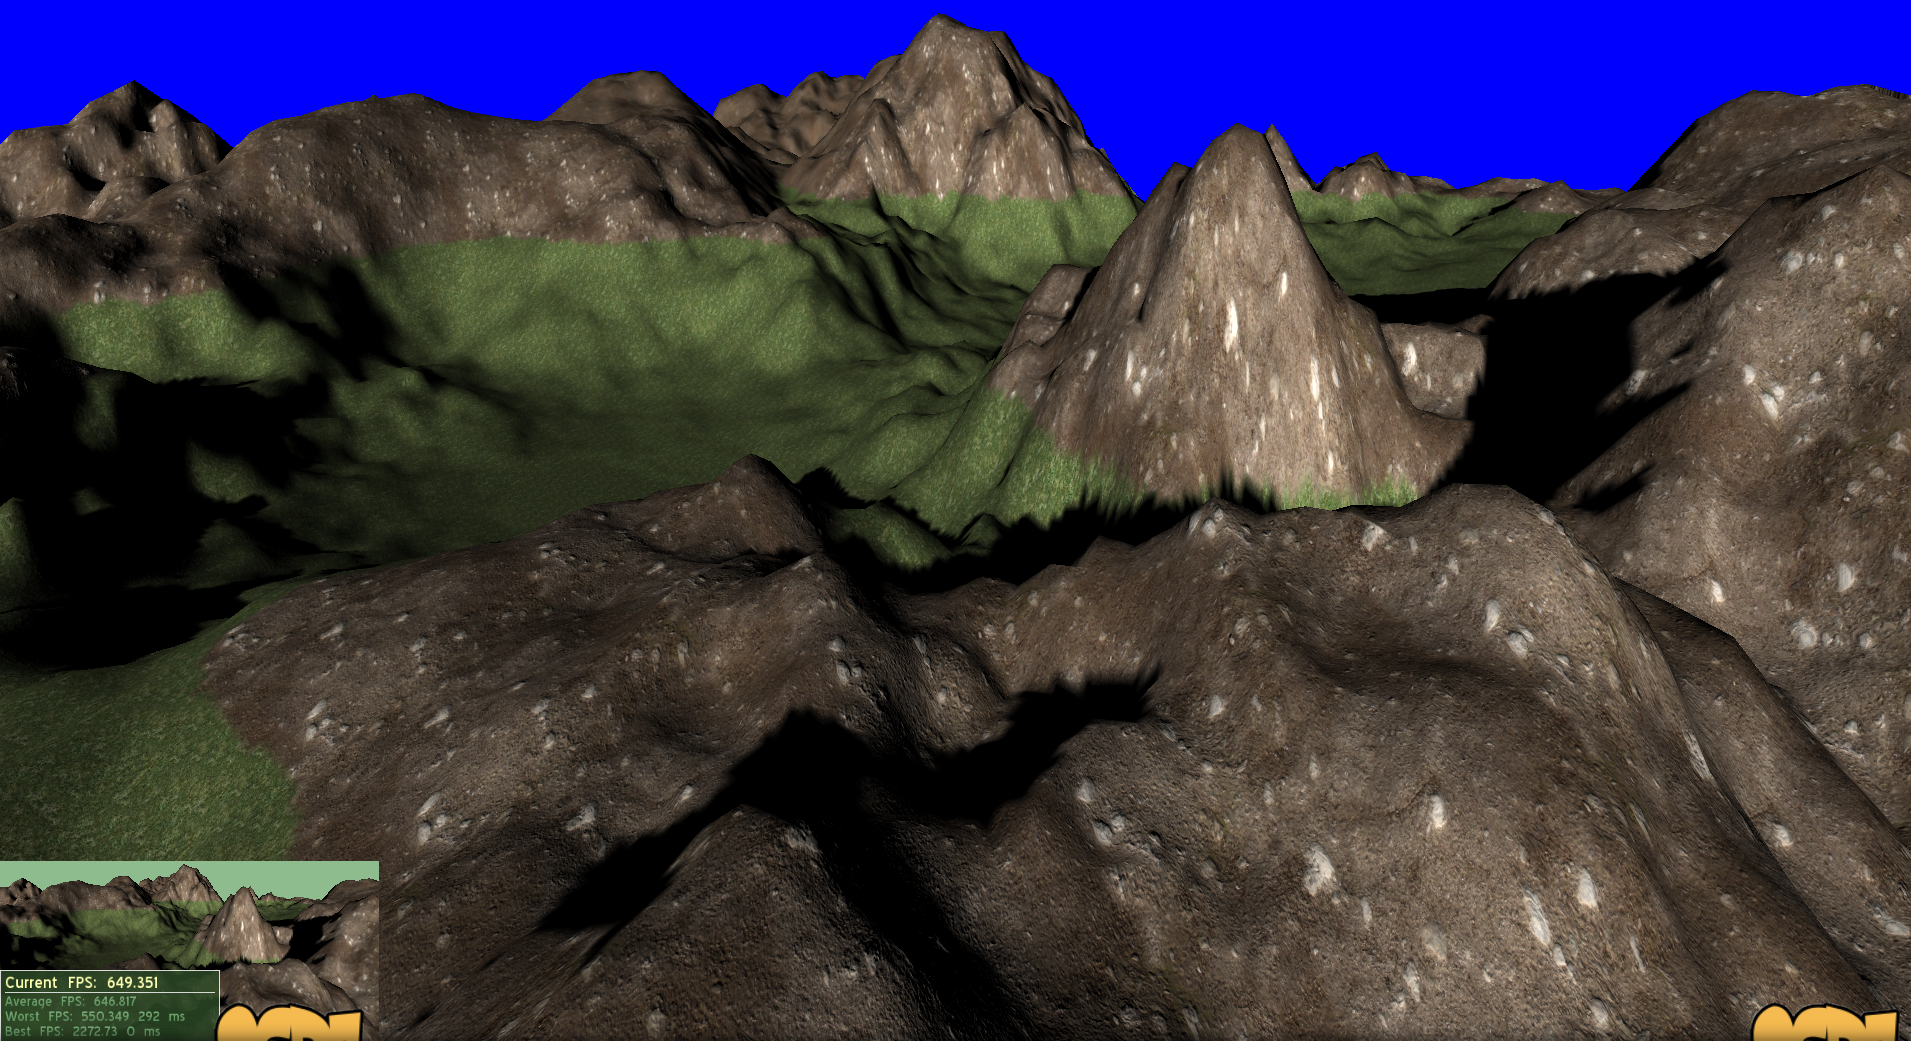
\includegraphics[width=8cm]{Ogre/1_Base_de_Ogre/5_Garder_les_pieds_sur_terre/images/Differentes_textures_selon_altitude1.png} %l'image est retaillée pour avoir une largeur de 10cm
\end{figure}




















\subsection{Pour aller plus loin}


Sur le même principe, nous allons voir comment appliquer deux textures différentes sur une petite largeur, à une altitude donnée.

Ceci peut être utile si vous voulez réaliser des étendues d'eau dans votre terrain : au bord de l'eau, il y a de la boue, un peu au-dessus, de la terre sèche, puis ensuite l'herbe reprend ses droits. C'est ce que nous allons faire, avec une opacité progressive, mais sans l'eau, ce sera pour plus tard.

Nous devons commencer par récupérer un pointeur sur notre seconde Blend Map pour pouvoir gérer la seconde texture en plus de la première. Il y a donc deux lignes à rajouter en conséquence avant les boucles.




\begin{lstlisting}[caption={Récupération des Blend Map pour le premier et le second terrain}]
Ogre::TerrainLayerBlendMap* blendMap1 = mTerrain->getLayerBlendMap(1);
Ogre::TerrainLayerBlendMap* blendMap2 = mTerrain->getLayerBlendMap(2);

float* pBlend1 = blendMap1->getBlendPointer();
float* pBlend2 = blendMap2->getBlendPointer();
\end{lstlisting}

Définissons aussi deux variables pour chacune des textures : la hauteur à laquelle se situe la texture et la largeur de la bande que l'on veut obtenir.

\begin{lstlisting}[caption={}]
Ogre::Real minHeight1 = 70;
Ogre::Real fadeDist1 = 40;
Ogre::Real minHeight2 = 70;
Ogre::Real fadeDist2 = 15;
\end{lstlisting}

Dans la boucle, on déclare trois variables : deux coordonnées du terrain et la transparence pour le point actuel.

\begin{lstlisting}[caption={}]
Ogre::Real terrainX, terrainY, transparence;
\end{lstlisting}

On récupère ensuite la hauteur du terrain comme précédemment.

\begin{lstlisting}[caption={}]
blendMap1->convertImageToTerrainSpace(x, y, &terrainX, &terrainY);
Ogre::Real height = mTerrain->getHeightAtTerrainPosition(terrainX, terrainY);
\end{lstlisting}

Ensuite, pour chaque texture, on calcule la différence entre la hauteur du point actuel et la hauteur que l'on veut pour la texture, divisée par la largeur de la bande. Si le point est censé être recouvert par la texture, ce nombre sera donc compris entre 0 et 1.

On utilise ensuite la méthode statique Clamp() qui a pour prototype :

\begin{lstlisting}[caption={Utilisation de la méthode statique Clamp()}]
static T Ogre::Math::Clamp(T val, T minval, T maxval)
\end{lstlisting}

Si val est inférieure à minval, la fonction retourne minval ; si val est supérieure à maxval, on retourne maxval. Si val est dans l'intervalle, on la retourne directement.

Comme on ne veut afficher que les points dont la valeur calculée précédemment est comprise entre 0 et 1, on va utiliser cette méthode pour ''couper'' toutes les valeurs en dehors de l'intervalle.

\begin{lstlisting}[caption={}]
transparence = (height - minHeight1) / fadeDist1;
transparence = Ogre::Math::Clamp(transparence, (Ogre::Real)0, (Ogre::Real)1);
\end{lstlisting}

Pour terminer, on multiplie transparence par 255 pour avoir une valeur comprise entre 0 et 255.

\begin{lstlisting}[caption={}]
*pBlend1++ = transparence * 255;
\end{lstlisting}

On observe que si transparence est à l'extérieur de l'intervalle [0 ; 1] après le premier calcul, Clamp retournera 0 ou 1. Quand on multiplie par 255, on obtient donc 0 ou 255, qui sont les deux valeurs pour lesquelles la texture est transparente. Mission accomplie !

On copie ces trois lignes pour la seconde texture, et on obtient le code suivant dans nos boucles :

\begin{lstlisting}[caption={}]
for (Ogre::uint16 y = 0; y < mTerrain->getLayerBlendMapSize(); ++y)
{
    for (Ogre::uint16 x = 0; x < mTerrain->getLayerBlendMapSize(); ++x)
    {
        Ogre::Real terrainX, terrainY, transparence;
        blendMap1->convertImageToTerrainSpace(x, y, &terrainX, &terrainY);
        Ogre::Real height = mTerrain->getHeightAtTerrainPosition(terrainX, terrainY);
        transparence = (height - minHeight1) / fadeDist1;
        transparence = Ogre::Math::Clamp(transparence, (Ogre::Real)0, (Ogre::Real)1);
        *pBlend1++ = transparence * 255;
        transparence = (height - minHeight2) / fadeDist2;
        transparence = Ogre::Math::Clamp(transparence, (Ogre::Real)0, (Ogre::Real)1);
        *pBlend2++ = transparence * 255;
    }
}
\end{lstlisting}

Pensez à mettre à jour la seconde Blend Map une fois que les modifications sont terminées :

\begin{lstlisting}[caption={}]
blendMap1->dirty();
blendMap2->dirty();
blendMap1->update();
blendMap2->update();
\end{lstlisting}




\subsubsection{Code}
Les seules choses à changer sont le plaquage de texture:


\begin{lstlisting}[caption={Plaquage de textures sur zone}]
...
    ///pour definir des bandes d'altitude avec une texture differente
    Ogre::Real minHeight1 = 70;
    Ogre::Real fadeDist1 = 40;
    Ogre::Real minHeight2 = 70;
    Ogre::Real fadeDist2 = 15;
    
    
    ///recuperation du blend map pour le premier terrain
    Ogre::TerrainLayerBlendMap* blendMap1 = mTerrain->getLayerBlendMap(1);/**<recuperation du blend map*/
    Ogre::TerrainLayerBlendMap* blendMap2 = mTerrain->getLayerBlendMap(2);/**<recuperation du blend map*/
    
    ///plaquage de la texture..
    float* pBlend1 = blendMap1->getBlendPointer();
    float* pBlend2 = blendMap2->getBlendPointer();
    ///..en fonction de l'altitude
    for (Ogre::uint16 y = 0; y < mTerrain->getLayerBlendMapSize(); ++y)
    {
        for (Ogre::uint16 x = 0; x < mTerrain->getLayerBlendMapSize(); ++x)
        {
            Ogre::Real terrainX, terrainY, transparence;
            
            blendMap1->convertImageToTerrainSpace(x, y, &terrainX, &terrainY);
            Ogre::Real height = mTerrain->getHeightAtTerrainPosition(terrainX, terrainY);
            
            transparence = (height - minHeight1) / fadeDist1;
            transparence = Ogre::Math::Clamp(transparence, (Ogre::Real)0, (Ogre::Real)1);
            *pBlend1++ = transparence * 255;
            
            transparence = (height - minHeight2) / fadeDist2;
            transparence = Ogre::Math::Clamp(transparence, (Ogre::Real)0, (Ogre::Real)1);
            *pBlend2++ = transparence * 255;
        }
    }
    
    blendMap1->dirty();/**<precise que les donnees de la blend Map st obsoletes*/
    blendMap1->update();/**<fait la mise a jour des donnees de la blend map*/
    blendMap2->dirty();/**<precise que les donnees de la blend Map st obsoletes*/
    blendMap2->update();/**<fait la mise a jour des donnees de la blend map*/ 
...
\end{lstlisting}



Et on obtiend:
\begin{figure}[hbtp]
\caption{Terrain.png}
\centering
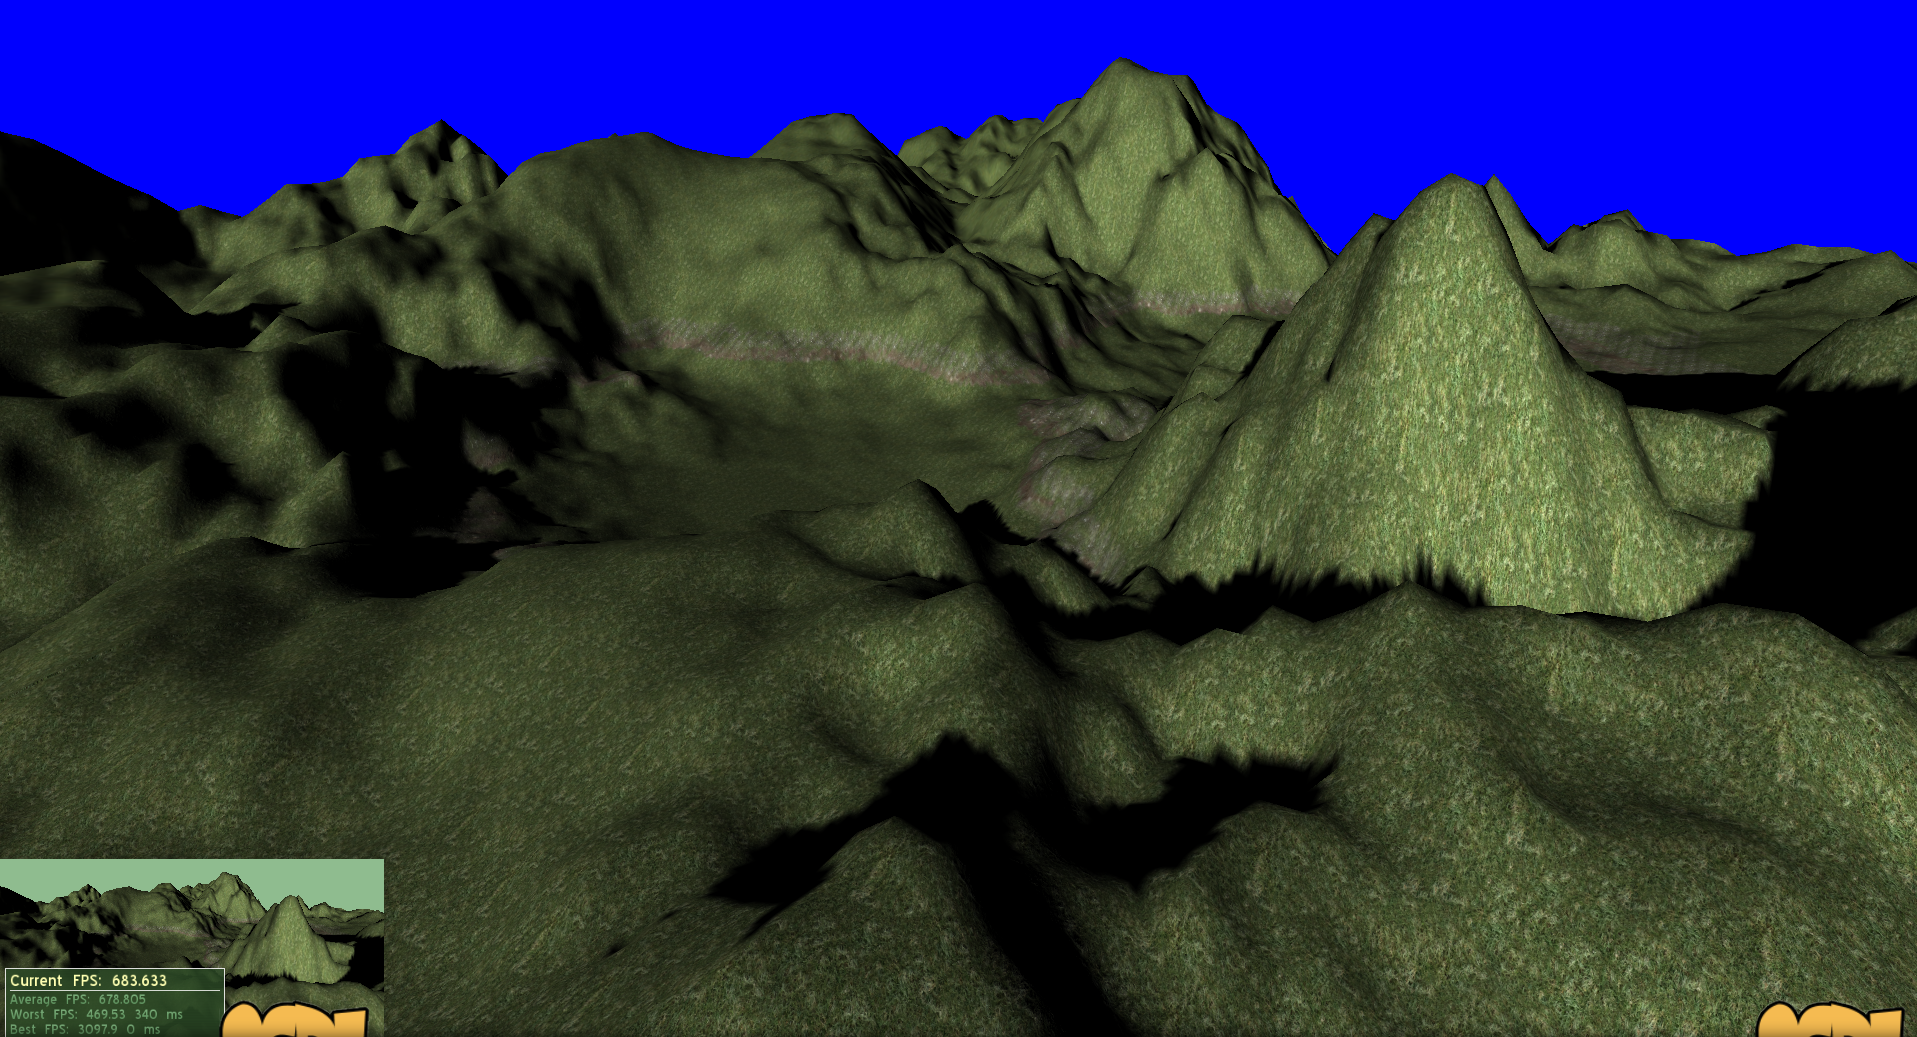
\includegraphics[width=8cm]{Ogre/1_Base_de_Ogre/5_Garder_les_pieds_sur_terre/images/Differentes_textures_selon_altitude2.png} %l'image est retaillée pour avoir une largeur de 10cm
\end{figure}








%140522
%A relire, corriger et indexer à partir d ici
%---------------------------------------------------------------------------------------------------------------
\section{Les groupes de terrains}

Un groupe de terrains\index{groupe de terrains} (ou TerrainGroup\index{TerrainGroup}) range les terrains comme dans un tableau à deux dimensions. Dans le groupe, tous les terrains doivent avoir la même taille, afin de pouvoir les aligner dans une grille.



\subsection{Création}

On commence par ajouter un include au début de la classe puis on remplace notre instance de Terrain par un TerrainGroup, ensuite on l'initialisera dans notre méthode createTerrain() :

\begin{lstlisting}[caption={TerrainGroup: include et création}]
#include <Ogre/Terrain/OgreTerrainGroup.h>
//...
Ogre::TerrainGroup *mTerrainGroup;
\end{lstlisting}

Après les lignes permettant de charger l'image heightmap dans la méthode createTerrain()\index{createTerrain()}, insérez les lignes suivantes.

\begin{lstlisting}[caption={}]
mTerrainGroup = OGRE_NEW Ogre::TerrainGroup(mSceneMgr, Ogre::Terrain::ALIGN_X_Z, img.getWidth(), 8000);

//On definit ensuite la position de l'origine du groupe de terrains
mTerrainGroup->setOrigin(Ogre::Vector3::ZERO);

//nom (et l'extension) que l'on veut attribuer a nos fichiers qui seront crees pour sauvegarder les terrains
mTerrainGroup->setFilenameConvention(Ogre::String("TerrainDuZero"), Ogre::String("dat"));
\end{lstlisting}

Les paramètres à fournir au TerrainGroup sont
\begin{itemize}
\item le Scene manager,
\item l'alignement du terrain\index{ALIGN\_X\_Z}\index{Terrain!ALIGN\_X\_Z}\index{alignement du terrain} par rapport au repère global (vous pouvez créer un terrain vertical, par exemple),
\item la taille des heightmaps utilisées\index{getWidth()}\index{heightmaps!getWidth()}, 
\item la taille d'un terrain.
\end{itemize}

On définit ensuite la position de l'origine du groupe de terrains\index{setOrigin()}\index{TerrainGroup!setOrigin()}, puis le nom\index{setFilenameConvention()}\index{TerrainGroup!setFilenameConvention()} (et l'extension) que l'on veut attribuer à nos fichiers qui seront créés pour sauvegarder les terrains par la suite.

Pour les données des terrains enregistrées dans un objet ImportData, nous allons modifier un peu le fonctionnement du programme. On récupère en fait directement une référence sur un ImportData fourni par le TerrainGroup\index{getDefaultImportSettings()}\index{TerrainGroup!getDefaultImportSettings()}, que l'on modifie directement et qui sera valable pour l'ensemble des terrains du groupe. à noter que la ligne de définition de la heightmap n'est plus utile ici, cela sera indiqué lors de la création des terrains.

\begin{lstlisting}[caption={}]
Ogre::Terrain::ImportData& imp = mTerrainGroup->getDefaultImportSettings();
imp.terrainSize = img.getWidth();
imp.worldSize = 8000;
imp.inputScale = 600;
imp.minBatchSize = 33;
imp.maxBatchSize = 65;
\end{lstlisting}

Il est maintenant temps de créer les terrains du groupe. On définit la taille du groupe et pour chaque case, on appelle une méthode definirTerrain() définie plus bas qui s'occupera de créer chaque terrain indépendamment.

\begin{lstlisting}[caption={Création des terrains du groupe}]
int largeur = 2, longueur = 2;

for(int x = 0; x < largeur; x++)
{
    for(int y = 0; y < longueur; y++)
    {
        definirTerrain(x, y);
    }
}
mTerrainGroup->loadAllTerrains(true);
\end{lstlisting}

Le groupe se charge pour terminer d'appeler les méthodes load()\index{load()} de chaque terrain à travers la méthode loadAllTerrains()\index{loadAllTerrains()}. Cette méthode prend un booléen en paramètre qui indique si le chargement doit être synchrone, c'est-à-dire exécuté dans un seul thread (le thread principal ici). Par défaut cette valeur est fausse, c'est-à-dire que les terrains sont chargés dans plusieurs threads si c'est possible.

Le chargement devient vite très lourd si l'on ajoute beaucoup de terrains aux groupes. Nous verrons plus bas comment accélérer le chargement.

Maintenant, nous devons écrire la méthode definirTerrain() qui utilise la méthode defineTerrain()\index{defineTerrain()}\index{TerrainGroup!defineTerrain()} de TerrainGroup. Celle-ci va prendre 3 paramètres : les deux coordonnées du terrain dans le groupe de terrains (sa position sur la grille, donc) et l'image heightmap utilisée pour ce terrain. Les coordonnées du terrain au sein du groupe peuvent être négatives.

Juste avant d'appeler le terrain, on va faire une vérification sur les coordonnées : si l'abscisse du terrain est impaire, on inverse l'image suivant l'axe Y, si l'ordonnée est impaire, on inverse l'image cette fois-ci selon l'axe X. Cela permet aux terrains du groupe de ne pas avoir de différence d'altitude lors des jointures. Si vous utilisez des heightmaps\index{heightmaps} différents sur les terrains du groupe (ce qui sera probablement le cas), vous devrez faire attention à ce que les altitudes des bords correspondent pour éviter les trous à ces endroits.

\begin{lstlisting}[caption={PremiereApplication.definirTerrain}]
void PremiereApplication::definirTerrain(int x, int y)
{
    Ogre::Image img;
    img.load("terrain.png", Ogre::ResourceGroupManager::DEFAULT_RESOURCE_GROUP_NAME);

    if(x % 2 != 0)
        img.flipAroundY();

    if(y % 2 != 0)
        img.flipAroundX();

    mTerrainGroup->defineTerrain(x, y, &img);
}
\end{lstlisting}

Une fois que les terrains sont chargés, il faut leur appliquer les textures définies. On utilise pour cela un itérateur sur le groupe de terrains et, pour chaque terrain, on appelle une méthode initBlendMaps() qui contient le code pour texturer les terrains.

\begin{lstlisting}[caption={}]
Ogre::TerrainGroup::TerrainIterator ti = mTerrainGroup->getTerrainIterator();

while(ti.hasMoreElements())
{
    Ogre::Terrain* t = ti.getNext()->instance;
    initBlendMaps(t);
}
\end{lstlisting}

La méthode initBlendMaps() contient uniquement du code que l'on a déjà vu mais que j'ai déplacé pour plus de clarté. Elle prend en paramètre le terrain dont on doit modifier les Blend maps.

\begin{lstlisting}[caption={}]
void PremiereApplication::initBlendMaps(Ogre::Terrain *terrain)
{
    Ogre::TerrainLayerBlendMap* blendMap1 = terrain->getLayerBlendMap(1);
    Ogre::TerrainLayerBlendMap* blendMap2 = terrain->getLayerBlendMap(2);
    Ogre::Real minHeight1 = 70;
    Ogre::Real fadeDist1 = 40;
    Ogre::Real minHeight2 = 70;
    Ogre::Real fadeDist2 = 15;
    float* pBlend1 = blendMap1->getBlendPointer();
    float* pBlend2 = blendMap2->getBlendPointer();

    for (Ogre::uint16 y = 0; y < terrain->getLayerBlendMapSize(); ++y)
    {
        for (Ogre::uint16 x = 0; x < terrain->getLayerBlendMapSize(); ++x)
        {
            Ogre::Real terrainX, terrainY, transparence;
            blendMap1->convertImageToTerrainSpace(x, y, &terrainX, &terrainY);
            Ogre::Real height = terrain->getHeightAtTerrainPosition(terrainX, terrainY);
            transparence = (height - minHeight1) / fadeDist1;
            transparence = Ogre::Math::Clamp(transparence, (Ogre::Real)0, (Ogre::Real)1);
            *pBlend1++ = transparence * 255;
            transparence = (height - minHeight2) / fadeDist2;
            transparence = Ogre::Math::Clamp(transparence, (Ogre::Real)0, (Ogre::Real)1);
            *pBlend2++ = transparence * 255;
        }
    }
    blendMap1->dirty();
    blendMap2->dirty();
    blendMap1->update();
    blendMap2->update();
}
\end{lstlisting}

Pour terminer, comme avec un terrain seul, on libère la mémoire utilisée par le TerrainGroup.

\begin{lstlisting}[caption={}]
mTerrainGroup->freeTemporaryResources();
\end{lstlisting}

Votre scène doit maintenant avoir une surface plus grande que la première fois (on a maintenant quatre terrains). Vous pouvez encore augmenter le nombre de terrains, mais attention, le temps de chargement augmente rapidement !



\subsection{Optimiser le temps de chargement}

Vous avez certainement remarqué que la génération du terrain prend un temps conséquent lorsque le groupe s'agrandit. La création du terrain à partir du fichier heightmap nécessite en effet de convertir les données de l'image en données exploitables par le moteur.

Afin de réduire le temps de chargement, il est possible d'enregistrer un fichier qui contient toutes les informations sur le terrain construit pour éviter de relire l'image à chaque lancement de l'application. L'inconvénient majeur est la place occupée par ces fichiers générés, qui contiennent beaucoup plus d'informations qu'une simple heightmap.

En regardant la création du groupe de terrains, vous voyez que l'on a défini une convention de nommage pour des fichiers, mais qui est pour l'instant inutilisée.

\begin{lstlisting}[caption={}]
mTerrainGroup->setFilenameConvention(Ogre::String("TerrainDuZero"), Ogre::String("dat"));
\end{lstlisting}

Cette ligne sert lors de la sauvegarde de fichiers de terrain : ceux-ci seront nommés en commen\c{c}ant par "TerrainDuZero" suivi d'un nombre permettant d'identifier le terrain, puis de l'extension de fichier "dat".

Pour utiliser la sauvegarde des terrains, nous allons ajouter un attribut mTerrainCreated à la classe PremiereApplication qui permettra de savoir si l'on a généré le terrain à partir d'une image ou bien si l'on a lu un fichier terrain. Dans le premier cas, on saura qu'à la fin de la méthode createTerrain() il faut penser à sauvegarder les fichiers de terrain pour le prochain lancement de l'application.

\begin{lstlisting}[caption={}]
bool mTerrainCreated;
\end{lstlisting}

Initialisez sa valeur à false au début de la méthode createTerrain().

Maintenant, dans notre méthode definirTerrain(), il faut vérifier si le fichier terrain existe déjà ou bien s'il faut faire la génération depuis le heightmap comme le faisait jusqu'alors. Dans le second cas, on passe la variable mTerrainCreated à true.

\begin{lstlisting}[caption={}]
void PremiereApplication::definirTerrain(int x, int y)
{
    if(Ogre::ResourceGroupManager::getSingleton().resourceExists(mTerrainGroup->getResourceGroup(), mTerrainGroup->generateFilename(x, y)))
    {
        mTerrainGroup->defineTerrain(x, y);
    }
    else
    {
        Ogre::Image img;
        img.load("terrain.png", Ogre::ResourceGroupManager::DEFAULT_RESOURCE_GROUP_NAME);

        if(x % 2 != 0)
            img.flipAroundY();

        if(y % 2 != 0)
            img.flipAroundX();

        mTerrainGroup->defineTerrain(x, y, &img);
        mTerrainCreated = true;
    }
}
\end{lstlisting}

Revenons sur la condition à tester pour vérifier l'existence du fichier généré.

Grâce au Ogre::ResourceGroupManager, on peut vérifier s'il existe une ressource précise dans l'ensemble des ressources chargées au démarrage du programme. Les paramètres de la méthode sont le groupe de ressources dans lequel on veut chercher la ressource ainsi que le nom du fichier recherché. Vous voyez que le nom du fichier généré par le groupe de terrains dépend de ses coordonnées X et Y, ainsi que de la convention que l'on a définie au début.

Si le fichier est trouvé, on appelle la méthode definieTerrain() avec seulement les coordonnées en paramètres. Dans ce cas, Ogre va aller chercher directement le fichier correspondant à ces coordonnées. Dans le cas contraire, on exécute le bloc que l'on avait précédemment et qui charge le terrain à partir de l'image de heightmap.

Il ne reste plus qu'à demander la sauvegarde des fichiers si l'on a généré les terrains juste avant de libérer les ressources dans la méthode createTerrain() :

\begin{lstlisting}[caption={}]
if(mTerrainCreated)
    mTerrainGroup->saveAllTerrains(true);
\end{lstlisting}


Lancez l'application, le temps de chargement doit être un peu plus long qu'auparavant car l'ordinateur sauvegarde en même temps les fichiers générés sur le disque. Une fois que l'application est lancée, fermez-la puis relancez-la. Le temps de chargement doit normalement être meilleur.

Vous devriez trouver les fichiers générés dans le dossier OgreSDK.media. Pour information, les miens font chacun une taille de 12 Mo.



























%---------------------------------------------------------------------------------------------------------------

\chapter{Une application \`a partir de z\'ero}

Apr\`es avoir vue le fonctionnement g\'en\'eral des classes de bases de Ogre, il est temps de s'attaquer au fonctionnement du moteur. Dans la suite de ce chapitre, nous allons apprendre \'a nous passer de la classe ExampleApplication pour la remplacer par notre propre classe d'initialisation du moteur.

\section{Pr\'eparation}

\subsection{Les \'etapes}

Pour que Ogre soit correctement initialis\'e et pr\`es \'à \^etre utilis\'e, on peut identifier les huits points suivants:
\begin{itemize}
- La cr\'eation d'un objet Root
- La d\'efinition des ressources \`a utiliser
- La cr\'eation du syst\`eme et de la fen\^etre de rendu (appel\'ee \italic{RenderWindow})
- L'initialisation des ressources 
- La cr\'eation de la sc\`ene 
- Le chargement \'eventuel des plugins additionnels
- La cr\'eation des frame listeners
- Le lancement de la boucle infinie
\end{itemize}

\subsection{Vocabulaire}

Le Root

Le Root est l'objet de base du moteur Ogre. C'est autour de lui que tout se construit et c'est donc lui qui doit-\^etre cr\'e\'e en premier. Son cr\'eation permet l'initialisation du moteur afin de pr\'eparer le terrain pour les objets qui vont venir graviter autour.

Les ressources

Nous allons travailler sur une application pour laquel la vitesse d'ex\'ecution est primordiale. Charger les ressources \'a la vol\'ee demande du temps \'a l'ordianteur (acc\`ees aux fichiers sur le disque dur, lecture des fichiers, allocation des ressources en m\'emoire et enfin chargement des donn\'ees en m\'emoire pour pouvoir les utiliser). Il est donc important d'effectuer toutes ces op\'erations au d\'emarrage du moteur (ou comme dans un jeu au chargement d'un nouveau niveau). Ainsi une fois que les ressources sont charg\'ees, plus besoin d'y toucher, on n'a plus qu'\'a s'occuper des m\'ecanismes du jeu. 

Le \italic{RenderWindow}

Un objet \italic{RenderWindow} repr\'esente la fen\^etre contenant la sc\`ene affich\'ee \'a l'\'ecran. Attention toutefois, on ne parle pas ici de la fen\^etre du syst\`eme d'exploitation mais du cadre dans lequel est rendu la sc\`ene. La diff\'erence est importante car si l'on programme un \'editeur de sc\`ene par exemple, la fen\^etre du programme contiendra non seulement la \italic{RenderWindow} mais aussi des menus et des boites \'a outils

La boucle infinie  



%---------------------------------------------------------------------------------------------------------------

\appendix

%\chapter{LaTeX}
\chapter{Latex}

\section{V\'erifier sa configuration latex}
Lors d'une importation de ce document sur un autre pc que celui utilis\'e pour \'ecrire ce document des probl\`emes peuvent appara\^itre lors de la compilation de ce fichier tex.\newline

Pour v\'erifier que aucun package latex ne manque cr\'eer un fichier tex et y copier/coller le code suivant. Ce code reprend tous les packages utilis\'es pour l'\'ecriture de ce pr\'esent document (prise de notes \'a partir du tutorial du site des z\'ero sur Ogre)










%----------------
\begin{lstlisting}[caption={Code Latex minimal pour tester les packages latex n\'ecessaires \'a la compilation du fichier ****-ergo.tex par texmaker}]

\documentclass[10pt,a4paper]{report}
\usepackage[latin1]{inputenc}
\usepackage{amsmath}
\usepackage{amsfonts}
\usepackage{amssymb}
\usepackage{hyperref} %pr inserer des liens internet

\usepackage{verbatim}%pour linsertion brute de commande LaTeX dans le texte
\usepackage{moreverb}

\usepackage[french]{babel}
\usepackage[latin1]{inputenc}

\usepackage{listings}
\usepackage{xcolor}

\usepackage{makeidx}

\title{OGRE}
\author{O}

\begin{document}
This is a MINIMUM WORKING EXAMPLE. hgf\newline

\'e
\`e
\^e
\newline

\'A
\`A
\^S
\end{document}

\end{lstlisting}




















%------------------------



\section{Caract\`eres accentu\'es}

Pour faire un \`{u}
\begin{verbatim}
\`{u}
\end{verbatim}


Pour faire un \^{a}
\begin{verbatim}
\^{a}
\end{verbatim}

Pour faire un \`{a}
\begin{verbatim}
\`{a} ou \`a
\end{verbatim}


Pour faire un \"o
\begin{verbatim}
\''{o} ou \"o
\end{verbatim}

Pour faire un \^{i}
\begin{verbatim}
\^{i}
\end{verbatim}

Pour faire un \`e
\begin{verbatim}
\`e
\end{verbatim}

Pour faire un \^e
\begin{verbatim}
\^e
\end{verbatim}

Pour faire un \'{e}
\begin{verbatim}
\'{e} ou \'e
\end{verbatim}

Pour faire un \c{c}
\begin{verbatim}
\c{c}
\end{verbatim}

Pour faire un \.o
\begin{verbatim}
\.{o} ou \.o
\end{verbatim}


Pour faire un \~u
\begin{verbatim}
\~{u} ou \~u
\end{verbatim}

Pour faire un \=o
\begin{verbatim}
\={o} ou \=o
\end{verbatim}


Pour faire un \^u
\begin{verbatim}
\^u
\end{verbatim}

Pour faire des guillemets
\begin{verbatim}
''guillemets''
\end{verbatim}


\subsection{M\'ethode alternative (non test\'ee)}

Il semble possible d'ins\'erer directement tous les caract\`eres fran\c{c}ais, pour d\'emo tester le code suivant:

\begin{lstlisting}[caption={Insertion de caract\`eres fran\c{c}ais}][language=latex]
\documentclass[10pt,a4paper]{article}
\usepackage[utf8]{inputenc}
\usepackage[T1]{fontenc}
\begin{document}
entrer des caracteres accentues francais
guillemets
\end{document}

\end{lstlisting}

Le probl\`eme est que cel\`a a des cons\'equences sur le code d\'ej\`a \'ecrit.



\section{Notes}
\subsection{Note dans la marge}
Une note dans la marge\marginpar{ceci est une note
dans la marge}
\subsection{Note de bas de marge}
Une note de bas de page\footnote{Comme celle-ci.}.



\section{Liens hyperlien}
Deux m\'ethodes diff\'erentes:

\begin{itemize}
\item Le lien est ajout\' e de mani\`ere brute:

\begin{lstlisting}[caption={Insertion de liens Internet}][language=latex]
ceci est un lien brut \url{http://estcequecestbientotleweekend.fr/}
\end{lstlisting}

et cel\`a donne ceci:\newline
ceci est un lien brut
\url{http://estcequecestbientotleweekend.fr/}\newline
\end{itemize}



\begin{itemize}
\item Un mot m\`ene vers le lien, ci-dessous un clic sur ''lien'' m\`ene au lien spécifi\'e

\begin{lstlisting}[caption={Insertion de liens Internet}][language=latex]
ceci est un lien \href{http://estcequecestbientotleweekend.fr/}{lien}
\end{lstlisting}

et cel\`a donne ceci:\newline
ceci est un \href{http://estcequecestbientotleweekend.fr/}{lien}
\end{itemize}






\section{Bloc comment\'e}
Un bloc comment\'e se fait avec le package verbatim
\begin{verbatim}
\begin{comment}
	bloc comment\'e
\end{comment}
\end{verbatim}



\section{Num\'erotation des chapitres et autres}
Apparemment le fait d'\'ecrire 

\begin{verbatim}
\section
\end{verbatim}

fait que la section sera num\'erot\'ee, 

\begin{verbatim}
\section*
\end{verbatim}

ne sera pas num\'erot\'ee.




\begin{comment}
\section{Underscore}
Il faut penser \`{a} \'echapper les underscore sinon la compilation plante. On \'echappe avec 
\end{comment}


\section{Insertion d'images}
Pour ins\'erer des images la m\'ethode suivie est la suivante:

\begin{lstlisting}[caption={Insertion d'image}][language=latex]
\usepackage{graphicx}

\begin{document}
	\begin{center}
	\includegraphics[scale=0.5]{monimage.jpg} 
	\end{center}
\end{document}

\end{lstlisting}






\section{Exemple d'insertion de code avec lstlisting}
L'insertion de code se fait grace aux packages:

\begin{lstlisting}
\usepackage{listings} %pr inserer du code
\usepackage{xcolor}
\end{lstlisting}

On peut ensuite d\'efinir certain param\`etres d'insertion
\begin{lstlisting}[caption={Commande pour sp\'ecifier les param\`etres d'insertion de code}] [language=tex]
\lstset{
basicstyle=\small, % print whole listing small
keywordstyle=\color{blue}\bfseries\underbar,
% underlined bold black keywords
identifierstyle=, % nothing happens
commentstyle=\color{white}, % white comments
stringstyle=\ttfamily, % typewriter type for strings
showstringspaces=false} % no special string spaces
\end{lstlisting}


\begin{lstlisting}
for i:=maxint to 0 do
begin
{ do nothing }
end;
Write('Case insensitive ');
Write('Pascal keywords.');
\end{lstlisting}


cf \url{http://tex.stackexchange.com/questions/21106/adding-c-code-in-latex}


\section{Cr\'eer un index}
Pour cr\'eer un index:
cf \url{http://www.tuteurs.ens.fr/logiciels/latex/makeindex.html}

pour que l'index soit g\'er\'e par TexMaker:
cf \url{http://www.xm1math.net/doculatex/makeindex.html}




%bizarrement le \part ci-dessous creee une entree ds la structure du document presentee par TexMaker
\section{Cr\'eer une annexe}

Pour cr\'er une annexe il faut utiliser la commande
\begin{lstlisting}[caption={Cr\'eer une annexe}] [language=latex]
\appendix		
%\chapter{Test}	% une "Annexe A Test" sera creee
\chapter{test}	% sera creee "A.1 test"
\end{lstlisting}


%l index sera ecrit ici
\printindex

\end{document}

